\chapter{赋范空间与内积空间}
\label{chap:normed-inner-product-spaces}

上一章的线性空间只有加法和数乘。借助它们可以判断一个向量能否由给定向量线性表示、表示是否唯一，却无法回答两个向量相差多少、一列近似是否趋于某个极限、两个方向是否垂直。本章给线性空间补上这两类度量结构：先用范数规定大小，再用内积规定角度。

本章分两步补上这些结构。前三节只用范数。第~\ref{sec:ls-normed-spaces}节给出范数的公理与例子，并用显式不等式比较常用的坐标范数，说明误差的数值依赖所选范数。第~\ref{sec:multivariable-limits-continuity}节用范数定义向量列与矩阵列的收敛、映射的联合极限与连续性，并证明闭有界集上的连续函数取到最值、一致连续。

第~\ref{sec:ls-finite-dimensional-normed-properties}节利用上一节的最值定理证明：有限维空间中任意两个范数等价，空间完备，绝对收敛的向量与矩阵级数收敛。在此基础上，矩阵范数衡量线性映射的最大放大倍数，对偶范数衡量误差受限时线性读取的最大变化，商范数衡量忽略一个子空间后剩下的大小。第~\ref{chap:linear-recurrence-stability}章的矩阵幂与Neumann级数、第~\ref{chap:stationary-iterations}章的迭代以及第~\ref{chap:multivariate-differentiation}章的微分，都使用这套分析基础。

范数不给出角度，一般范数下向子空间的最近点也可能不唯一。后三节引入内积来回答这些问题。第~\ref{sec:ls-inner-product-spaces}节从公理推出长度、夹角和Cauchy--Schwarz不等式，并用Gram矩阵记录一组向量的两两内积。第~\ref{sec:ls-orthogonality-and-projection}节研究正交分解、标准正交基和正交投影，证明正交投影是子空间中唯一的最近点。第~\ref{sec:ls-adjoints}节用内积把上一章的线性泛函表示为与固定向量的内积，并把对偶映射改写成内积空间之间的伴随。

本章依赖前两章的线性运算、基与坐标，以及一元分析中的数列极限、确界和最值定理（第~\ref{sec:multivariable-limits-continuity}节开头说明所用的结论）。全章只讨论有限维空间；收敛与连续性适用于一般映射，不限于线性映射。无限维的函数空间中，范数等价、完备性和最近点存在都可能失败，那里的理论可参考\BookChapterRef{chap:functional-analysis-and-approximation}{卷四“函数空间”一章}。

% 赋范空间：范数与距离；收敛、极限与连续性；有限维赋范空间的性质（范数等价、完备性、级数、矩阵范数、对偶范数、商范数），只讨论有限维情形。

\section{范数与距离}
\label{sec:ls-normed-spaces}

用多项式近似一个函数时，要估计误差有多大；迭代产生一列近似时，要判断它是否趋于某个对象。这些问题都需要先规定向量的大小。第~\ref{chap:linear-operations}章用$\ell_1$、$\ell_2$、$\ell_\infty$范数度量$\mathbb R^d$中数组的大小，本节把这种度量推广到一般线性空间。

本节先给出范数的公理和例子，再用显式不等式比较常用的坐标范数。这里只用到线性运算与标量不等式。下一节用范数定义收敛、映射的极限与连续性；第~\ref{sec:ls-finite-dimensional-normed-properties}节再证明有限维空间中任意两个范数等价、空间完备，并讨论矩阵、线性泛函和商空间的大小。本章只讨论有限维空间。

\subsection{范数的定义与示例}
\label{sec:ls-normed-space-definition}

\paragraph{范数的定义}
第~\ref{chap:linear-operations}章的$\ell_1$、$\ell_2$、$\ell_\infty$范数算法不同，却有几条共同性质。大小非负，只有零向量的大小为零。向量放大$c$倍时，大小变为原来的$|c|$倍。两个向量之和的大小不超过各自大小之和。这些性质只涉及加法和数乘，因此可以直接作为一般线性空间上“大小”的要求。
\begin{definition}[赋范空间]
\label{def:ls-normed-space}
\label{def:functional-normed-space}
设$V$是实线性空间。映射$\lVert\cdot\rVert:V\to[0,\infty)$若对任意$\bm x,\bm y\in V$与$c\in\mathbb R$满足
\begin{enumerate}
 \item 正定性：$\lVert\bm x\rVert=0$当且仅当$\bm x=\bm0$；
 \item 齐次性：$\lVert c\bm x\rVert=|c|\,\lVert\bm x\rVert$；
 \item 三角不等式：$\lVert\bm x+\bm y\rVert\leq\lVert\bm x\rVert+\lVert\bm y\rVert$，
\end{enumerate}
就称为$V$上的\term{范数}（norm）；配备范数的线性空间$(V,\lVert\cdot\rVert)$称为\term{赋范空间}（normed space）。
\end{definition}
范数诱导距离$d(\bm x,\bm y)=\lVert\bm x-\bm y\rVert$。这个距离非负，只在$\bm x=\bm y$时为零，对称，并满足$d(\bm x,\bm z)\leq d(\bm x,\bm y)+d(\bm y,\bm z)$。这四条正是度量空间对距离的要求，所以赋范空间是一类特殊的度量空间；一般度量空间可参考\BookChapterRef{chap:metric-spaces}{卷四“度量空间”一章}。它的距离还与线性运算相容：平移不改变距离，缩放按同一比例改变距离。

三角不等式还能反过来控制长度之差。把它用于$\bm x=(\bm x-\bm y)+\bm y$，得$\lVert\bm x\rVert-\lVert\bm y\rVert\leq\lVert\bm x-\bm y\rVert$；交换$\bm x,\bm y$，又得$\lVert\bm y\rVert-\lVert\bm x\rVert\leq\lVert\bm x-\bm y\rVert$。两式合起来就是反向三角不等式
\begin{equation}
 \bigl|\lVert\bm x\rVert-\lVert\bm y\rVert\bigr|\leq\lVert\bm x-\bm y\rVert.
 \label{eq:ls-reverse-triangle}
\end{equation}
即两个向量的长度之差不超过差向量的长度。下一节用它说明范数随向量收敛。

\paragraph{坐标范数的公理检验}
\label{sec:ls-norms-distances}
\label{sec:linear-algebra-distance-relations}
现在检验第~\ref{sec:ls-vector-operations}节的$p$范数确实是范数。非负性、正定性与齐次性可以从公式直接读出，需要证明的只有三角不等式。$p=1$和$p=\infty$时，它由实数的三角不等式逐坐标得到，细节见下面Minkowski不等式的证明。$1<p<\infty$时，需要先建立Hölder不等式。

\paragraph{Hölder不等式}
Hölder不等式用一对$p$范数与$q$范数控制两个向量逐坐标乘积之和。两个指数须满足共轭条件$1/p+1/q=1$。
\begin{theorem}[有限维Hölder不等式]
\label{thm:linear-algebra-holder}
设$1\leq p,q\leq\infty$且$1/p+1/q=1$（约定$1/\infty=0$），则$|\bm x^\top\bm y|\leq\lVert\bm x\rVert_p\lVert\bm y\rVert_q$。
\end{theorem}
\begin{proof}
先设$1<p,q<\infty$，分三步证明。

第一步，证明Young不等式：对$u,v\geq0$，
\[
 uv\leq\frac{u^p}{p}+\frac{v^q}{q}.
\]
$u=0$时左侧为零，不等式成立。$u>0$时令$t=v/u^{p-1}\geq0$。由$1/p+1/q=1$得$(p-1)q=p$，于是$v^q=t^qu^p$、$uv=tu^p$，不等式化为
\[
 u^p\Bigl(\frac1p+\frac{t^q}{q}-t\Bigr)\geq0.
\]
函数$f(t)=1/p+t^q/q-t$的导数$t^{q-1}-1$在$0<t<1$时为负、在$t>1$时为正，所以$f$在$t\geq0$上的最小值是$f(1)=1/p+1/q-1=0$，不等式成立。

第二步，在单位尺度下求和。若$\bm x$或$\bm y$为零向量，结论两侧都为零。否则令$u_j=|x_j|/\lVert\bm x\rVert_p$、$v_j=|y_j|/\lVert\bm y\rVert_q$，则$\sum_ju_j^p=\sum_jv_j^q=1$。对每个$j$用Young不等式再求和，得
\[
 \sum_ju_jv_j\leq\frac1p\sum_ju_j^p+\frac1q\sum_jv_j^q=\frac1p+\frac1q=1.
\]

第三步，恢复尺度。上式两边乘以$\lVert\bm x\rVert_p\lVert\bm y\rVert_q$，再用$|\bm x^\top\bm y|\leq\sum_j|x_j||y_j|$，即得
\[
 |\bm x^\top\bm y|\leq\sum_j|x_j||y_j|\leq\lVert\bm x\rVert_p\lVert\bm y\rVert_q.
\]

端点情形直接估计。$p=1$、$q=\infty$时，
\[
 \sum_j|x_j||y_j|\leq\Bigl(\max_j|y_j|\Bigr)\sum_j|x_j|=\lVert\bm x\rVert_1\lVert\bm y\rVert_\infty;
\]
$p=\infty$、$q=1$时交换两个向量的角色。
\end{proof}
$p=q=2$时，它给出$|\bm x^\top\bm y|\leq\lVert\bm x\rVert_2\lVert\bm y\rVert_2$。第~\ref{sec:ls-inner-product-definition}节将只用内积公理，对任一内积证明同样形式的不等式，即Cauchy--Schwarz不等式。

\paragraph{Minkowski不等式}
有了Hölder不等式，就可以对一般的$p$证明三角不等式。做法是把$|x_j+y_j|^p$拆成两个乘积之和，再对每一部分使用Hölder不等式。
\begin{theorem}[有限维Minkowski不等式]
\label{thm:linear-algebra-minkowski}
设$\bm x,\bm y\in\mathbb R^d$，$1\leq p\leq\infty$，则
\[
 \lVert\bm x+\bm y\rVert_p\leq\lVert\bm x\rVert_p+\lVert\bm y\rVert_p.
\]
\end{theorem}
\begin{proof}
先处理两个端点。$p=1$时，对每个坐标使用实数的三角不等式，再求和，得到
\[
 \sum_j|x_j+y_j|\leq\sum_j|x_j|+\sum_j|y_j|.
\]
$p=\infty$时，对每个$j$都有
\[
 |x_j+y_j|\leq\lVert\bm x\rVert_\infty+\lVert\bm y\rVert_\infty.
\]
左侧对$j$取最大值，就得到所需结论。

下面设$1<p<\infty$。若$\bm x+\bm y=\bm0$，左侧为零，结论成立；以下设和向量非零。取$q=p/(p-1)$，则$1/p+1/q=1$。对每个坐标有
\[
 \begin{aligned}
 |x_j+y_j|^p
 &=|x_j+y_j|^{p-1}|x_j+y_j|\\
 &\leq |x_j+y_j|^{p-1}(|x_j|+|y_j|).
 \end{aligned}
\]
令$s_j=|x_j+y_j|^{p-1}$，把这些数排成向量$\bm s$。由于$(p-1)q=p$，它的$q$范数为
\[
 \begin{aligned}
 \lVert\bm s\rVert_q
 &=\Bigl(\sum_j|x_j+y_j|^p\Bigr)^{1/q}\\
 &=\lVert\bm x+\bm y\rVert_p^{p-1}.
 \end{aligned}
\]
把逐坐标的不等式求和，并对含$|x_j|$和含$|y_j|$的两部分分别使用Hölder不等式，得到
\[
 \begin{aligned}
 \lVert\bm x+\bm y\rVert_p^p
 &\leq\sum_js_j|x_j|+\sum_js_j|y_j|\\
 &\leq\lVert\bm s\rVert_q
       \bigl(\lVert\bm x\rVert_p+\lVert\bm y\rVert_p\bigr)\\
 &=\lVert\bm x+\bm y\rVert_p^{p-1}
       \bigl(\lVert\bm x\rVert_p+\lVert\bm y\rVert_p\bigr).
 \end{aligned}
\]
两边除以正数$\lVert\bm x+\bm y\rVert_p^{p-1}$，即得结论。
\end{proof}
结合前面直接读出的三条性质，每个$p$范数都满足定义~\ref{def:ls-normed-space}。特别地，欧氏长度满足三角不等式。

\paragraph{其他空间上的范数}
除$p$范数外，前面还出现过别的范数。同形矩阵上的Frobenius范数，就是把矩阵元素排成向量后的$2$范数；诱导矩阵范数将在第~\ref{sec:ls-matrix-norms}节定义并验证。

在一般线性空间上，最直接的做法是借助坐标。若$\lVert\cdot\rVert_\star$是$\mathbb R^d$上的范数，$\mathcal B$是$V$的基，则$\lVert\bm v\rVert=\lVert[\bm v]_{\mathcal B}\rVert_\star$是$V$上的范数，因为坐标映射是保持线性组合的双射。也可以不经过坐标，直接用对象本身的性质规定范数。下面在$P_k$上各举一例。
\begin{example}[多项式空间上的两个范数]
\label{ex:ls-polynomial-norms}
对$p=a_0+a_1t+\cdots+a_kt^k$，可以看系数，也可以看函数在区间$[0,1]$上的取值，由此得到两个规则：
\[
\begin{gathered}
p\mapsto\max_{0\leq j\leq k}|a_j|,\\
p\mapsto\lVert p\rVert_\infty=\max_{t\in[0,1]}|p(t)| .
\end{gathered}
\]

第一个规则正是坐标$(a_0,\ldots,a_k)$在基$(1,t,\ldots,t^k)$下的$\ell_\infty$范数，按上面借助坐标的方法，它是范数。第二个规则不经过坐标，需要逐条检验公理。齐次性在每个$t$处成立，取最大值后仍成立。对三角不等式，每个$t$都满足$|p(t)+q(t)|\leq|p(t)|+|q(t)|\leq\lVert p\rVert_\infty+\lVert q\rVert_\infty$，左侧再对$t$取最大值即可。正定性依赖多项式的代数性质：次数不超过$k$的非零多项式至多有$k$个根，不能在整个区间$[0,1]$上为零。

所以两个规则都是$P_k$上的范数。前者借助坐标，后者直接用函数值，检验时只需用到多项式本身的性质。
\end{example}

有时只关心向量的一部分信息。这时可以去掉正定性，只保留非负性、齐次性与三角不等式，得到的尺度称为\term{半范数}（seminorm）。半范数可能把两个不同的点判为距离为零。
\begin{example}[只看第一个坐标的半范数]
\label{ex:ls-seminorm-first-coordinate}
在$\mathbb R^2$上只用第一个坐标衡量大小，令$p(\bm x)=|x_1|$。半范数要求的三条性质都由实数绝对值的性质得到：$p(\bm x)\geq0$，$p(c\bm x)=|cx_1|=|c|\,p(\bm x)$，并且$p(\bm x+\bm y)=|x_1+y_1|\leq|x_1|+|y_1|=p(\bm x)+p(\bm y)$。缺少的是正定性：非零向量$(0,1)^\top$满足$p\bigl((0,1)^\top\bigr)=0$。

因此$p$是半范数而不是范数。用它度量距离时，$(0,0)^\top$与$(0,1)^\top$的距离为$p\bigl((0,-1)^\top\bigr)=0$，两个不同的点被视为没有差别，第二个坐标上的差别完全被忽略。
\end{example}
因此使用半范数之前，须先说明哪些差别被有意忽略。

\subsection{常用坐标范数的比较}
\label{sec:ls-error-scale-comparison}

不同的$p$范数给同一个向量的大小不同。误差估计常常要在两种范数之间换算，因此需要知道它们最多相差多少倍。对$\mathbb R^d$中的坐标范数，这个倍数可以由有限求和直接算出。
\begin{theorem}[坐标范数的比较]
\label{thm:ls-coordinate-norm-comparison}
设$1\leq p\leq q\leq\infty$，约定$1/\infty=0$。对$\bm x\in\mathbb R^d$，
\[
 \lVert\bm x\rVert_q\leq\lVert\bm x\rVert_p\leq d^{1/p-1/q}\lVert\bm x\rVert_q.
\]
\end{theorem}
\begin{proof}
$\bm x=\bm0$时三项都为零，下设$\bm x\neq\bm0$。

左侧。令$\bm u=\bm x/\lVert\bm x\rVert_p$，则$\lVert\bm u\rVert_p=1$，所以每个$|u_j|\leq1$。$q=\infty$时这就是$\lVert\bm u\rVert_\infty\leq1$。$q<\infty$时，由$|u_j|\leq1$与$q\geq p$得$|u_j|^q\leq|u_j|^p$，求和得$\lVert\bm u\rVert_q^q\leq\lVert\bm u\rVert_p^p=1$。两种情形都有$\lVert\bm u\rVert_q\leq1$，两边乘以$\lVert\bm x\rVert_p$即得。

右侧。$p=q$时显然。$q=\infty$时，$\sum_j|x_j|^p\leq d\,\lVert\bm x\rVert_\infty^p$，开$p$次方即得。设$p<q<\infty$，取$r=q/p>1$，其共轭指数满足$1/r'=1-p/q$。对向量$(|x_1|^p,\ldots,|x_d|^p)^\top$与全$1$向量使用Hölder不等式（定理~\ref{thm:linear-algebra-holder}），
\[
 \sum_j|x_j|^p\cdot1\leq\Bigl(\sum_j|x_j|^{q}\Bigr)^{p/q}d^{\,1-p/q}=\lVert\bm x\rVert_q^p\,d^{\,1-p/q}.
\]
开$p$次方，得$\lVert\bm x\rVert_p\leq d^{1/p-1/q}\lVert\bm x\rVert_q$。
\end{proof}
最常用的是$p,q\in\{1,2,\infty\}$的情形：
\[
 \begin{gathered}
 \lVert\bm x\rVert_\infty\leq\lVert\bm x\rVert_2\leq\sqrt d\,\lVert\bm x\rVert_\infty,\\
 \lVert\bm x\rVert_2\leq\lVert\bm x\rVert_1\leq\sqrt d\,\lVert\bm x\rVert_2,\\
 \lVert\bm x\rVert_\infty\leq\lVert\bm x\rVert_1\leq d\,\lVert\bm x\rVert_\infty.
 \end{gathered}
\]
下面在示例~\ref{ex:ls-p-norms}的向量上核对前两行。
\begin{example}[范数比较的数值核对]
\label{ex:ls-norm-comparison-check}
取$d=2$与$\bm x=(3,-4)^\top$。示例~\ref{ex:ls-p-norms}已经算出$\lVert\bm x\rVert_1=7$，$\lVert\bm x\rVert_2=5$，$\lVert\bm x\rVert_\infty=4$。代入前两行，比较常数分别为$\sqrt2$：
\[
 \begin{gathered}
 4\leq5\leq4\sqrt2\approx5.66,\\
 5\leq7\leq5\sqrt2\approx7.07.
 \end{gathered}
\]
四个不等式都成立，而且右侧的界离实际值不远。同一个误差$\bm x$在三种范数下读出$4$、$5$、$7$三个不同的数，比较定理保证的是这些读数之间的倍数不超过与维数有关的常数。
\end{example}
两侧的常数一般都不能改进，取等号的向量很简单。
\begin{example}[比较常数的取等]
\label{ex:ls-l1-linf-constants}
两个极端的向量分别使两侧取等号：只有一个非零坐标的$\bm e_1$，和各坐标一样大的全$1$向量$\bm 1$。对每个$p$都有$\lVert\bm e_1\rVert_p=1$，所以$\bm e_1$使左侧取等号。另一方面，$p<\infty$时$\lVert\bm 1\rVert_p=d^{1/p}$，又$\lVert\bm 1\rVert_\infty=1$，因此在约定$1/\infty=0$下总有$\lVert\bm 1\rVert_p=d^{1/p-1/q}\lVert\bm 1\rVert_q$，右侧取等号。

大小全部集中在一个坐标上时，各范数读数相同；各坐标绝对值相等时，读数相差最大。例如$\ell_1$与$\ell_\infty$之间的常数$1$与$d$分别由$\bm e_1$和$\bm 1$达到，都不能改进。
\end{example}
右侧的常数随维数增长。维数较大时，换用范数带来的倍数差别不能在误差估计中忽略；固定维数下的比较式也不能当作对所有维数一致成立的界。这里只比较了有明确公式的坐标范数。有限维空间上任意两个范数都只相差常数倍（定理~\ref{thm:ls-norm-equivalence}），这一结论的证明要用到闭有界集上连续函数的最值，在第~\ref{sec:multivariable-norm-equivalence}节给出。

\section{收敛、极限与连续性}
\label{sec:multivariable-limits-continuity}

上一节的范数度量一个向量的大小。本节用它描述“接近”：一列向量或矩阵怎样趋于极限，映射的输出怎样随输入的接近而接近。向量与矩阵的分量都只有有限个，许多结论可以逐个坐标归结为一元的结果：数列极限的运算法则、闭区间上的Bolzano--Weierstrass定理与最值定理、一致连续性，以及实数列的柯西收敛准则。这些一元结论及其证明可参考\BookChapterRef{chap:limits-continuity}{卷一“极限与连续”一章}，本章用到时只说明所用的结论和条件。

本节先固定欧氏范数和Frobenius范数，建立逐坐标判据、映射的极限与连续性，以及闭有界集上连续函数的基本性质。换用任意范数时这些性质是否保留，留到下一节证明，以免在范数等价的证明中循环使用结论。这些概念适用于一般映射，不限于线性映射；后面的矩阵幂、迭代和多元微分都以它们为基础。

\subsection{向量列与矩阵列的收敛}
\label{sec:ls-finite-dimensional-sequences}

一元数列$a_k\to a$的意思是误差$|a_k-a|$趋于零。向量有多个坐标，要求的是整个误差向量的大小趋于零。在$\mathbb R^d$中用欧氏范数度量这个大小，在$\mathbb R^{m\times n}$中用Frobenius范数。
\begin{definition}[向量列与矩阵列的收敛]
\label{def:multivariable-sequence-convergence}
设$\bm x_k,\bm x\in\mathbb R^d$。若实数列$\lVert\bm x_k-\bm x\rVert_2\to0$，就称向量列$(\bm x_k)$\emph{收敛}到$\bm x$，记为$\bm x_k\to\bm x$。同样，同形矩阵列$\bm A_k$与矩阵$\bm A\in\mathbb R^{m\times n}$满足$\lVert\bm A_k-\bm A\rVert_{\mathrm F}\to0$时，称$\bm A_k\to\bm A$。
\end{definition}
序列中各项的维数或形状都相同，候选极限也属于同一个空间。复向量与复矩阵可以把每个元素拆成实部和虚部，看作维数加倍的实向量，作同样的讨论。

\paragraph{逐坐标判据}
欧氏误差与各坐标误差之间有显式的夹逼关系，所以向量收敛可以逐个坐标检查。
\begin{theorem}[收敛等价于逐坐标收敛]
\label{thm:multivariable-coordinatewise-convergence}
$\bm x_k\to\bm x$当且仅当每个坐标$x_{k,j}\to x_j$（$j=1,\ldots,d$）；$\bm A_k\to\bm A$当且仅当每个元素$(\bm A_k)_{i,j}\to a_{i,j}$。
\end{theorem}
\begin{proof}
由定理~\ref{thm:ls-coordinate-norm-comparison}，
\[
 \max_j|x_{k,j}-x_j|\leq\lVert\bm x_k-\bm x\rVert_2\leq\sqrt d\,\max_j|x_{k,j}-x_j|.
\]
左侧不等式说明，欧氏误差趋于零时，每个坐标误差都趋于零。反过来，设每个坐标误差都趋于零。给定$\varepsilon>0$，对每个$j$取$N_j$，使$k>N_j$时$|x_{k,j}-x_j|<\varepsilon$；令$N=\max_jN_j$，则$k>N$时$\max_j|x_{k,j}-x_j|<\varepsilon$，由右侧不等式，欧氏误差小于$\sqrt d\,\varepsilon$。把矩阵的元素按固定顺序排成向量，Frobenius范数就是欧氏范数，矩阵的结论随之得到。
\end{proof}
证明中取$N=\max_jN_j$要求坐标只有有限个。换用别的范数或别的基是否改变结论，在第~\ref{sec:multivariable-norm-equivalence}节回答。

\paragraph{极限的唯一性与运算}
极限若存在则唯一：若$\bm x_k\to\bm x$且$\bm x_k\to\bm y$，则
\[
 \lVert\bm x-\bm y\rVert_2\leq\lVert\bm x-\bm x_k\rVert_2+\lVert\bm x_k-\bm y\rVert_2\to0.
\]
由反向三角不等式~\eqref{eq:ls-reverse-triangle}，$\bm x_k\to\bm x$时还有$\lVert\bm x_k\rVert_2\to\lVert\bm x\rVert_2$。收敛序列有界：取$N$使$k>N$时$\lVert\bm x_k-\bm x\rVert_2<1$，则所有项的长度不超过$\max\{\lVert\bm x_1\rVert_2,\ldots,\lVert\bm x_N\rVert_2,\lVert\bm x\rVert_2+1\}$。

线性运算和乘法都保持极限。设$\bm x_k\to\bm x$、$\bm y_k\to\bm y$，实数列$c_k\to c$，则
\[
 \bm x_k+\bm y_k\to\bm x+\bm y,\qquad c_k\bm x_k\to c\bm x,\qquad\bm x_k^\top\bm y_k\to\bm x^\top\bm y;
\]
若矩阵列$\bm A_k\to\bm A$、$\bm B_k\to\bm B$且形状相容，则$\bm A_k\bm B_k\to\bm A\bm B$。理由相同：结果的每个坐标或元素都是有限个标量数列的和与积，由一元数列的运算法则逐个得到极限，再用逐坐标判据。

\subsection{开集、闭集与有界集}
\label{sec:multivariable-open-closed-sets}

讨论映射的极限与连续性时，先要说明输入在什么样的集合里变化：基点周围是否留有向各个方向移动的余地，集合是否包含它边界上的点，集合是否伸向无穷远。这三个问题分别由开集、闭集与有界集回答。本小节在$\mathbb R^d$中用欧氏距离叙述，矩阵空间按Frobenius范数同样定义。

\paragraph{开球与开集}
以$\bm a$为心、半径为$r>0$的\emph{开球}是
\[
 B(\bm a,r)=\{\bm x:\lVert\bm x-\bm a\rVert_2<r\},
\]
即与$\bm a$的距离小于$r$的全部点。$d=1$时它是开区间$(a-r,a+r)$，$d=2$时是不含边界圆的圆盘。含有某个开球$B(\bm a,r)$的集合称为$\bm a$的一个\emph{邻域}；说“$\bm a$附近”某性质成立，就是指它在$\bm a$的某个邻域内成立。
\begin{definition}[开集、闭集与有界集]
\label{def:multivariable-open-closed-bounded}
设$K\subseteq\mathbb R^d$。
\begin{enumerate}
 \item 若$K$中每一点$\bm a$都有某个开球$B(\bm a,r)\subseteq K$，就称$K$为\emph{开集}。
 \item 若补集$\mathbb R^d\setminus K$是开集，就称$K$为\emph{闭集}。
 \item 若存在$R$，使$\lVert\bm x\rVert_2\leq R$对一切$\bm x\in K$成立，就称$K$\emph{有界}。
\end{enumerate}
\end{definition}
开集中的每一点都被同一集合的点包围：从这一点出发，向任何方向走足够小的一步都还在集合里。后面在开集上求导数，正是要用到这一点，因为双侧差商需要向两侧都能移动。半径$r$可以随点改变，越靠近边界，能取的半径越小。

闭集与开集不是对立的两类。整个空间$\mathbb R^d$与空集既开又闭；平面上的半开带$\{(x,y):0\leq x<1\}$既不开也不闭，因为它含有边界$x=0$上的点，却不含边界$x=1$上的点。闭集的直观意义是“包含自己的全部边界点”，下面的序列判据把这一点说清楚。

有界性只说明集合不伸向无穷远。它与中心的选取无关：若$K\subseteq B(\bm a,r)$，则由三角不等式，$K$中的点满足$\lVert\bm x\rVert_2\leq\lVert\bm a\rVert_2+r$。

\paragraph{聚点、孤立点与边界点}
若以$\bm a$为心的每个开球都含有$D$中不同于$\bm a$的点，就称$\bm a$是$D$的\emph{聚点}。聚点可以不属于$D$；它的意义在于，$D$中的点能从$\bm a$以外任意接近$\bm a$，因此可以讨论$\bm x\to\bm a$时的极限。$D$中不是聚点的点称为\emph{孤立点}：它周围某个小球内只有它自己属于$D$。

若以$\bm a$为心的每个开球既含$K$中的点、又含补集中的点，就称$\bm a$是$K$的\emph{边界点}。例如开圆盘的边界点就是单位圆上的点，它们都不属于开圆盘，却都是开圆盘的聚点。

\paragraph{闭集的序列判据}
与实轴上的闭集一样，$\mathbb R^d$中的闭集也可以用序列刻画：闭集包含其中任何收敛序列的极限。
\begin{lemma}[闭集的序列判据]
\label{lem:multivariable-closed-sequence}
$K\subseteq\mathbb R^d$是闭集，当且仅当：$K$中任何收敛序列的极限仍属于$K$。
\end{lemma}
\begin{proof}
设$K$闭，$\bm x_k\in K$，$\bm x_k\to\bm x$。若$\bm x\notin K$，补集是开集，存在开球$B(\bm x,r)$与$K$不相交；而$k$充分大时$\bm x_k\in B(\bm x,r)$，矛盾。反过来，设$K$包含其中收敛序列的极限。若补集不是开集，就有$\bm x\notin K$，使每个$B(\bm x,1/k)$都含有$K$中的点$\bm x_k$；于是$\bm x_k\to\bm x$，$\bm x$应属于$K$，矛盾。
\end{proof}
\begin{example}[圆盘与矩阵球]
\label{ex:multivariable-open-closed-sets}
比较平面上的开圆盘$\{x^2+y^2<1\}$与闭圆盘$\{x^2+y^2\leq1\}$，再看矩阵空间中的球$\{\bm X\in\mathbb R^{2\times2}:\lVert\bm X-\bm I_2\rVert_{\mathrm F}\leq1/2\}$，就能看到三个定义怎样分别检验。

开圆盘中的点$\bm x$满足$\lVert\bm x\rVert_2<1$。取$r=1-\lVert\bm x\rVert_2$，由三角不等式，$B(\bm x,r)$含于开圆盘，所以开圆盘是开集。它却不是闭集：序列$(1-1/k,0)$留在开圆盘中，极限$(1,0)$却不属于它；同样，边界圆上的点都是开圆盘的聚点。闭圆盘的情形相反。若闭圆盘中的序列$\bm x_k\to\bm x$，由$\lVert\bm x_k\rVert_2\leq1$与范数的收敛得$\lVert\bm x\rVert_2\leq1$，再由序列判据知闭圆盘是闭集。矩阵球按同样的论证是闭集，它又含于以零矩阵为心、半径$\lVert\bm I_2\rVert_{\mathrm F}+1/2$的球内，因而有界。

所以开圆盘开而不闭，闭圆盘与矩阵球闭且有界。开圆盘缺少的边界点仍是它的聚点，因此函数的定义域是开圆盘时，也可以在这些不属于定义域的点处讨论极限。
\end{example}

开圆盘缺少的恰好是它的边界圆。一般地，把$K$中序列所有可能的极限都补进来，得到$K$的\emph{闭包}
\[
 \overline K=\{\bm x\in\mathbb R^d:\text{存在}\bm x_k\in K\text{使}\bm x_k\to\bm x\}.
\]
取常数序列可知$K\subseteq\overline K$；$\overline K$中多出的点都是$K$的聚点，所以$\overline K$就是$K$与它全部聚点的并。闭包本身是闭集：若$\bm y_k\in\overline K$且$\bm y_k\to\bm y$，对每个$k$取$\bm x_k\in K$使$\lVert\bm x_k-\bm y_k\rVert_2<1/k$，则$\bm x_k\to\bm y$，于是$\bm y\in\overline K$，再用序列判据。另一方面，任何包含$K$的闭集都含有$K$中序列的极限，因而含有$\overline K$。所以闭包是包含$K$的最小闭集，$K$闭当且仅当$\overline K=K$。例如开圆盘的闭包是闭圆盘。

三种说法从不同角度描述同一件事：邻域描述一点周围的情形，边界点同时贴近集合与补集，闭包则是把边界上缺少的点补齐以后的集合。

\subsection{映射的联合极限}
\label{sec:multivariable-joint-limit-section}

本小节与下一小节研究映射$F:D\to W$，其中$D\subseteq V$。$V$与$W$取$\mathbb R^d$或矩阵空间，分别配欧氏范数或Frobenius范数；记号$\lVert\cdot\rVert$按所在空间理解。输出为实数（$W=\mathbb R$）时，$F$是多元标量函数；输出为向量时是向量值映射；输入为矩阵时，例如$\bm X\mapsto\bm X^{-1}$，就是矩阵的函数。下面的许多例子取标量输出，因为困难都来自输入的多个坐标。

\paragraph{多元标量函数}
多元标量函数在每个输入点给出一个实数。$d=2$时这类函数最容易画出来：把$f(x,y)$当作水平位置$(x,y)$上方的高度，所有点$(x,y,f(x,y))$组成一张曲面，称为函数的图像。
\begin{definition}[多元标量函数]
\label{def:multivariable-scalar-function}
设$d$为正整数、$D\subseteq\mathbb R^d$。映射$f:D\to\mathbb R$称为多元标量函数；它把整个输入点$\bm x=(x_1,\ldots,x_d)^\top$映为一个实数$f(\bm x)$。
\end{definition}
例如$f(x,y)=x^2+xy+y^2$在$(1,2)$处取值$1+2+4=7$。观察这类函数常用两种办法。
第一种是切片：固定$y=2$，得到一元函数$x\mapsto x^2+2x+4$。几何上，这是用竖直平面$y=2$去截曲面，截出一条曲线；它只反映原函数在一条直线上的取值。
第二种是等值曲线：把函数值相同的点连起来。例如$x^2+xy+y^2=7$是平面上一个经过$(1,2)$的倾斜椭圆，就像地图上的等高线。

后文的偏导数就是切片曲线的斜率，梯度则与等值曲线的方向有关。但切片只看一条直线。极限与连续性要回答的是：在整个平面中趋近基点时，函数值怎样变化。

\subsubsection{极限的定义}
\label{sec:multivariable-joint-limits}

一元时，$x\to a$只能从左右两侧靠近；在平面中，输入可以沿直线、抛物线、螺旋线等路径趋近基点。极限的定义必须用一个条件同时控制所有这些输入，不能按路径分别选择误差范围。做法是只看输入到基点的距离。

一元极限中，条件$0<|x-a|<\delta$表示$x$落在$a$两侧、半径为$\delta$的小区间内且不等于$a$。在平面上，与之对应的是以$\bm a$为圆心、半径为$\delta$的圆盘去掉圆心；在$\mathbb R^d$中则是去心的球。

欧氏距离$\lVert\bm x-\bm a\rVert_2$同时控制各坐标的偏移，用它代替$|x-a|$，就得到多元极限的邻域条件；输出的误差用输出空间的范数度量。设$F:D\to W$，$\bm a$是$D$的聚点。这个条件保证$\bm x$确实能在定义域内趋近$\bm a$。
\begin{definition}[映射的极限]
\label{def:multivariable-limit}
若对每个$\varepsilon>0$，都存在$\delta>0$，使得
\[
 \bm x\in D,\quad 0<\lVert\bm x-\bm a\rVert<\delta
 \quad\Longrightarrow\quad \lVert F(\bm x)-\bm L\rVert<\varepsilon,
\]
则称$F$在$\bm x\to\bm a$时的极限为$\bm L$，记为$\lim_{\bm x\to\bm a}F(\bm x)=\bm L$。标量函数$f$的情形中，输出误差就是$|f(\bm x)-L|$。
\end{definition}
定义中的$\delta$只依赖$\varepsilon$（以及固定的$f$与$\bm a$），不依赖输入从哪个方向来。只要点进入半径为$\delta$的去心球，函数值就必须落在$L$的$\varepsilon$范围内；点沿直线、沿曲线还是来回跳动地进入都一样。各坐标可以按不同速度趋近，行进方向也可以随位置改变，这些情形都由同一个$\delta$覆盖。这样定义的极限也称联合极限，以区别于只沿某条路径或逐个坐标取的极限。

\subsubsection{极限的判据}
\label{sec:multivariable-limit-criteria}

极限的定义要求一个误差半径同时控制全部趋近方式，直接验证往往不方便。本小节给出几种判据：序列判据把极限化为序列的收敛，路径检验与累次极限可以用来否定极限的存在，统一误差估计则用来证明极限存在。

\paragraph{序列判据}
与一元情形一样，$\lim_{\bm x\to\bm a}F(\bm x)=\bm L$当且仅当：任意满足$\bm x_n\in D\setminus\{\bm a\}$、$\bm x_n\to\bm a$的序列都有$F(\bm x_n)\to\bm L$。
证明只需把一元序列判据中的$|x_n-a|$换成$\lVert\bm x_n-\bm a\rVert$。

由逐坐标判据（定理~\ref{thm:multivariable-coordinatewise-convergence}），向量值或矩阵值映射的极限为$\bm L$，当且仅当每个输出分量的极限是$\bm L$的相应分量。这里分解的是输出。分别固定输入的坐标则是另一回事：它只检查若干种趋近方式，不能保证联合极限存在，下面的例子说明了这一点。

\paragraph{路径检验}
沿一条路径趋近基点时取出的点列只是这类序列的特例。由此可知路径检验能做什么、不能做什么。若沿两条路径得到不同的极限，就有两个序列的函数值趋于不同的数，联合极限不存在。反过来，只验证有限条路径，甚至验证全部过基点的直线，都没有覆盖全部序列，不能据此断定极限存在。

先看第一种情形：两条直线就足以否定联合极限。
\begin{example}[沿不同直线得到不同极限]
\label{ex:multivariable-path-limits}
令$f(0,0)=0$，非原点处令$f(x,y)=xy/(x^2+y^2)$。
沿直线$y=kx$（$x\neq0$）代入，得到
\[
 f(x,kx)=\frac{kx^2}{x^2+k^2x^2}=\frac{k}{1+k^2}.
\]
这个值不随$x$变化，却随斜率$k$变化：沿$x$轴（$k=0$）为$0$，沿$y=x$为$1/2$，沿$y=-x$为$-1/2$；沿$y$轴同样为$0$。
所以$f$的值只取决于点所在的方向，不取决于离原点多远。原点附近再小的圆盘里，$f$仍然取遍$-1/2$到$1/2$之间的值，原点处没有联合极限。

另一方面，固定$y=c$时，$x\mapsto f(x,c)$在$c\neq0$时是分母不为零的有理函数，在$c=0$时恒为$0$，都是连续的；固定$x$同理。于是$f$的每条坐标切片都连续，$f$却在原点不联合连续。
\end{example}

第二种情形更隐蔽：所有直线给出相同的极限，联合极限仍可能不存在。
\begin{example}[所有直线极限相同而联合极限不存在]
\label{ex:multivariable-parabola-path-limit}
令$g(0,0)=0$，并在非原点处令
\[
 g(x,y)=\frac{x^2y}{x^4+y^2}.
\]
沿$y=kx$，当$k\neq0$时$g(x,kx)=kx/(x^2+k^2)\to0$；
当$k=0$或沿竖直轴时，函数恒为$0$。所有直线给出的极限都是$0$。
可是沿抛物线$y=x^2$，$g(x,x^2)=x^4/(2x^4)=1/2$。更一般地，沿$y=cx^2$代入得到常数$c/(1+c^2)$，因此原点处没有联合极限。

直线检验失败的原因如下。对$x\neq0$，直线$y=kx$可以写成$y=(k/x)x^2$，相当于取$c=k/x$；靠近原点时$c\to\infty$，函数值$c/(1+c^2)\to0$。函数值为$1/2$的“山脊”沿抛物线$y=x^2$弯进原点，每条固定直线最终都离开山脊，进入函数值很小的区域。
\end{example}

因此路径检验只能否定联合极限。要证明联合极限存在，需要像后面的示例~\ref{ex:multivariable-distance-bound-limit}那样，给出对所有路径同时有效的误差估计。
图~\ref{fig:analysis-process-joint-limit-paths}把直线路径和弯曲路径画在同一函数上，可以看到只检查直线会遗漏哪种趋近方式。
\begin{figure*}[!htbp]
 \centering
 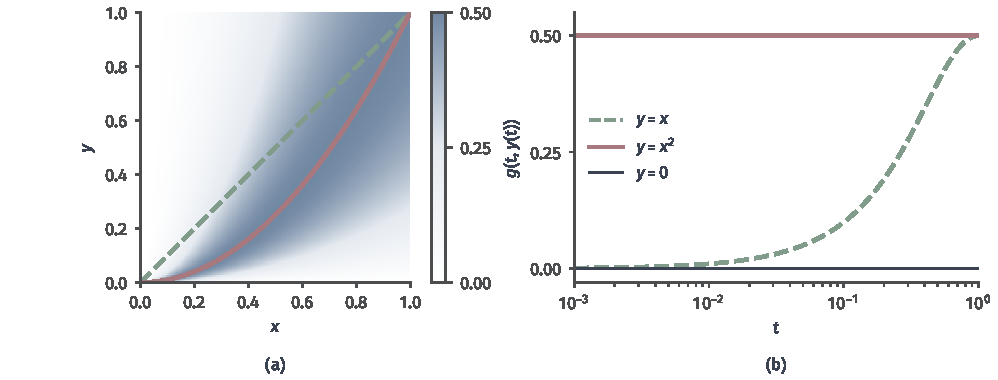
\includegraphics[width=169.0mm]{figures/00-shared/mathematical-preliminaries-upper/00-shared/matplotlib/chapter3-concept-processes/joint-limit-paths.pdf}
 \caption{取前例$g(x,y)=x^2y/(x^4+y^2)$，原点另置零。(a) 第一象限的函数值及三条路径，色阶固定为$0$至$1/2$。(b) 沿$y=0$、$y=x$分别趋零，沿$y=x^2$恒为$1/2$；横轴为正参数$t$的对数刻度，向左趋近原点。不同路径极限足以否定联合极限，有限条路径不能反向证明存在。}
 \label{fig:analysis-process-joint-limit-paths}
\end{figure*}

\paragraph{累次极限与联合极限}
另一种常见做法是逐个坐标取极限，称为累次极限。先令$y\to0$、再令$x\to0$，得到
\[
 \lim_{x\to0}\lim_{y\to0}f(x,y).
\]
内层固定$x\neq0$，让$y$单独趋于$0$；得到一个关于$x$的函数后，外层再让$x$趋于$0$。整个过程从不要求两个坐标同时趋近，因此它与联合极限是不同的问题。
对示例~\ref{ex:multivariable-path-limits}中的$f$，固定$x\neq0$时$f(x,y)\to0$，再令$x\to0$仍为$0$；交换次序同样得到$0$。两个次序的累次极限都为$0$，联合极限却不存在。

累次极限的结果还可能依赖取极限的次序。
\begin{example}[两个次序的累次极限不相等]
\label{ex:multivariable-iterated-limits-differ}
在非原点处令$h(x,y)=x^2/(x^2+y^2)$。固定$x\neq0$而令$y\to0$，得到$x^2/x^2=1$；固定$y\neq0$而令$x\to0$，得到$0$。再取外层极限，
\[
 \begin{gathered}
\lim_{x\to0}\lim_{y\to0}h(x,y)=1\\
\lim_{y\to0}\lim_{x\to0}h(x,y)=0.
 \end{gathered}
\]
内层先把一个坐标压到零，相当于先走到某条坐标轴附近，再沿坐标轴靠近原点。$h$在$x$轴上恒为$1$、在$y$轴上恒为$0$，两种次序因而给出不同结果。
\end{example}

两个例子说明：两个次序的累次极限相等，不足以推出联合极限存在；改变次序也可能改变累次极限。

反方向在补充条件下成立。若联合极限$\lim_{(x,y)\to(0,0)}f(x,y)=L$存在，并且对充分接近$0$的每个$x\neq0$，内层极限$\lim_{y\to0}f(x,y)$都存在，则累次极限$\lim_{x\to0}\lim_{y\to0}f(x,y)$也存在且等于$L$。理由是：给定$\varepsilon>0$，取联合极限定义中的$\delta$；当$0<|x|<\delta/2$、$0<|y|<\delta/2$时$|f(x,y)-L|<\varepsilon$，令$y\to0$，内层极限与$L$相差不超过$\varepsilon$。

\paragraph{统一误差估计}
要证明联合极限存在，可以寻找只依赖距离的上界。若$|f(\bm x)-L|$不超过一个只与$\lVert\bm x-\bm a\rVert_2$有关、并随距离趋于零的量，所有路径就同时受到控制。
\begin{example}[用距离上界证明联合极限]
\label{ex:multivariable-distance-bound-limit}
在非原点处考虑$x^2y/(x^2+y^2)$。由$|xy|\leq(x^2+y^2)/2$，有
\[
 \left|\frac{x^2y}{x^2+y^2}\right|
 =|x|\cdot\frac{|xy|}{x^2+y^2}
 \leq \frac{|x|}{2}
 \leq\frac12\sqrt{x^2+y^2}.
\]
给定$\varepsilon>0$，取$\delta=2\varepsilon$，则距离原点小于$\delta$的非原点都满足误差小于$\varepsilon$，因此原点处极限为$0$。

改用极坐标$(x,y)=(r\cos\theta,r\sin\theta)$，同一函数等于$r\cos^2\theta\sin\theta$，绝对值不超过$r$。这个界对所有$\theta$同时成立，给出同样的结论。
\end{example}

极坐标估计有效，关键在于这个界与角度无关。若只固定$\theta$再令$r\to0$，检查的仍然只是直线。
\begin{example}[固定角度的极坐标检验]
\label{ex:multivariable-polar-fixed-angle}
对示例~\ref{ex:multivariable-parabola-path-limit}中的$g$，代入$(x,y)=(r\cos\theta,r\sin\theta)$得到
\[
 g=\frac{r\cos^2\theta\sin\theta}{r^2\cos^4\theta+\sin^2\theta}.
\]
固定$\theta$再令$r\to0$：$\sin\theta\neq0$时分母趋于$\sin^2\theta$而分子趋于$0$，$\sin\theta=0$时函数恒为$0$，结果总是$0$。
但对每个小的$r>0$，可以取满足$\sin\theta=r\cos^2\theta$的角度。此时分子等于$r^2\cos^4\theta$、分母等于$2r^2\cos^4\theta$，函数值恰为$1/2$。这个角度随$r$改变，对应的点$(r\cos\theta,r\sin\theta)$满足$y=r^2\cos^2\theta=x^2$，正好落在抛物线上。
\end{example}

因此用极坐标证明联合极限时，需要一个对全部$\theta$同时成立、并随$r\to0$趋于零的界。

\subsection{连续性}
\label{sec:multivariable-continuity}

\subsubsection{连续性的定义}
\label{sec:multivariable-continuity-definition}

有了联合极限，就可以定义连续：输入联合趋近基点时，输出趋于基点处的值。定义形式与一元连续性相同，只是把$|x-a|$换成输入、输出空间中的距离。
\begin{definition}[映射的连续性]
\label{def:multivariable-scalar-continuity}
设$F:D\to W$、$\bm a\in D$。若对每个$\varepsilon>0$都存在$\delta>0$，使
\[
 \bm x\in D,\quad\lVert\bm x-\bm a\rVert<\delta
 \Longrightarrow \lVert F(\bm x)-F(\bm a)\rVert<\varepsilon,
\]
则称$F$在$\bm a$处连续；在$D$上每点连续时称$F$为连续映射，标量输出时也称连续函数。
\end{definition}
条件中允许$\bm x=\bm a$。在聚点处，这等价于联合极限等于$F(\bm a)$；在孤立点处，取足够小的$\delta$使球内只有$\bm a$，定义自动成立。与极限一样，$F$连续当且仅当每个输出分量连续。
几何上，连续意味着曲面在$\bm a$上方没有裂缝或跳跃：从任何方向走近，高度都平稳地接近$f(\bm a)$。
连续函数的每条坐标切片都连续，但反过来不成立：示例~\ref{ex:multivariable-path-limits}中各条切片都连续，函数在原点却不连续。

\subsubsection{连续性的性质}
\label{sec:multivariable-continuity-properties}

连续性在常用运算下保持。下面逐条检验和、差、数乘、积、商、乘积型运算与复合，再用它们说明求逆在可逆矩阵上连续。

\paragraph{和的连续性}
设$f,g$在$\bm a$处连续。由三角不等式，
\[
 |(f+g)(\bm x)-(f+g)(\bm a)|\leq|f(\bm x)-f(\bm a)|+|g(\bm x)-g(\bm a)|.
\]
给定$\varepsilon>0$，分别取使两个误差都小于$\varepsilon/2$的半径，其中较小的半径就满足$f+g$的连续性要求。

\paragraph{差的连续性}
相减时两项的误差仍按三角不等式相加：$|(f-g)(\bm x)-(f-g)(\bm a)|\leq|f(\bm x)-f(\bm a)|+|g(\bm x)-g(\bm a)|$。取与和相同的半径，即得$f-g$在$\bm a$处连续。

\paragraph{数乘的连续性}
对固定实数$c$，有$|cf(\bm x)-cf(\bm a)|=|c|\,|f(\bm x)-f(\bm a)|$。$c\neq0$时，把$f$的误差控制在$\varepsilon/|c|$以内即可；$c=0$时$cf$是常函数，结论直接成立。

\paragraph{积的连续性}
若$f,g$在$\bm a$处连续，乘积的误差可以拆成两项：
\[
 f(\bm x)g(\bm x)-f(\bm a)g(\bm a)
 =f(\bm x)\bigl(g(\bm x)-g(\bm a)\bigr)+g(\bm a)\bigl(f(\bm x)-f(\bm a)\bigr).
\]
由$f$的连续性，$\bm x$足够靠近$\bm a$时$|f(\bm x)|\leq|f(\bm a)|+1$，第一项的因子$f(\bm x)$有界；两个括号又都趋于零，所以$fg$在$\bm a$处连续。这与一元的乘积极限法则是同一个论证。

坐标函数$\bm x\mapsto x_j$连续，因为$|x_j-a_j|\leq\lVert\bm x-\bm a\rVert_2$。多元多项式由坐标函数和常数经有限次加法与乘法得到，因此连续，例如$x^2+xy+y^2$。

\paragraph{商的连续性}
除法还要防止分母变为零。若再设$g(\bm a)\neq0$，由$g$的连续性，可以取一个小球使其中$|g(\bm x)|>|g(\bm a)|/2$，即$g$在基点附近远离零。于是
\[
 \left|\frac1{g(\bm x)}-\frac1{g(\bm a)}\right|
 =\frac{|g(\bm x)-g(\bm a)|}{|g(\bm x)|\,|g(\bm a)|}
 \leq\frac{2|g(\bm x)-g(\bm a)|}{g(\bm a)^2}\longrightarrow0,
\]
所以$1/g$在$\bm a$处连续，再用积的连续性得到$f/g$连续。分母非零的条件不能省略，否则商在基点没有定义；由此，有理函数在分母非零处连续。

\paragraph{内积与矩阵乘法}
向量值与矩阵值映射的乘积同样保持连续。若$F,G$在$\bm a$处连续，取值为同维向量，则$\bm x\mapsto F(\bm x)^\top G(\bm x)$在$\bm a$处连续；若$F,G$取矩阵值且形状相容，则$\bm x\mapsto F(\bm x)G(\bm x)$在$\bm a$处连续。理由是结果的每个元素都是有限个分量乘积之和，由和与积的连续性及逐分量判据得到。

\paragraph{复合映射}
若$F:D\to W$在$\bm a$处连续，映射$G$在$F(\bm a)$处连续，且$F$在$\bm a$附近的输出都在$G$的定义域内，则$G\circ F$在$\bm a$处连续。
证明分两步控制误差。给定$\varepsilon>0$，先由$G$的连续性取$\eta>0$，使中间值与$F(\bm a)$相差小于$\eta$时，$G$的输出误差小于$\varepsilon$；再由$F$的连续性取$\delta>0$，使输入距离小于$\delta$时，$F$的输出与$F(\bm a)$相差小于$\eta$。合并两步，$\lVert\bm x-\bm a\rVert<\delta$时就有$\lVert G(F(\bm x))-G(F(\bm a))\rVert<\varepsilon$。
例如$e^{-(x^2+y^2)}$和$\sqrt{1+x^2+y^2}$都是一元连续函数与多项式的复合，因而在整个平面上连续。

\paragraph{逆映射}
矩阵的函数也可以用这些规则检验。记$\mathcal G=\{\bm X\in\mathbb R^{n\times n}:\det\bm X\neq0\}$。由定理~\ref{thm:ls-adjugate-identity}，在$\mathcal G$上
\[
 \bm X^{-1}=\frac{\operatorname{adj}(\bm X)}{\det\bm X}.
\]
$\det\bm X$与$\operatorname{adj}(\bm X)$的每个元素都是$\bm X$各元素的多项式，因而连续；在$\mathcal G$上分母非零，由商的连续性，$\bm X^{-1}$的每个元素都连续。由逐分量判据，求逆$\bm X\mapsto\bm X^{-1}$在可逆矩阵集合上连续。

\subsubsection{一致连续与Lipschitz连续}
\label{sec:multivariable-uniform-lipschitz}

连续性允许$\delta$随基点改变。有时需要在整个定义域上统一控制误差，或者给出误差的数量关系。
\begin{definition}[一致连续与Lipschitz连续]
\label{def:ls-lipschitz}
设$F:D\to W$。若对每个$\varepsilon>0$存在不依赖基点的$\delta>0$，使$\bm x,\bm y\in D$、$\lVert\bm x-\bm y\rVert<\delta$时$\lVert F(\bm x)-F(\bm y)\rVert<\varepsilon$，就称$F$在$D$上\term{一致连续}。若存在常数$L\geq0$，使
\[
 \lVert F(\bm x)-F(\bm y)\rVert\leq L\lVert\bm x-\bm y\rVert\qquad(\bm x,\bm y\in D),
\]
就称$F$在$D$上\term{Lipschitz连续}，$L$称为Lipschitz常数。若每点都有一个邻域，使$F$在该邻域与$D$的交上Lipschitz连续，就称$F$\emph{局部Lipschitz连续}。
\end{definition}
Lipschitz连续蕴含一致连续：取$\delta=\varepsilon/L$（$L=0$时任取）即可。反过来不成立：$\sqrt x$在$[0,1]$上连续，下一小节将说明它一致连续，但$|\sqrt x-\sqrt0|/|x-0|=1/\sqrt x$在$x\to0^+$时无界，没有Lipschitz常数。范数本身是Lipschitz连续的，由反向三角不等式，常数为$1$。这里只说明误差界的含义；第~\ref{chap:multivariate-differentiation}章将用导数求出可微映射的Lipschitz常数。

\subsection{闭有界集上的连续函数}

连续性的一个重要用途是保证最值存在。机器学习中常在一块参数区域内最小化损失；如果最小值根本取不到，“求最小点”就没有对象。
一元情形中，闭区间上的连续函数一定取到最值，关键事实是闭区间内任意点列都有收敛于该区间内的子列。本小节先把这一子列性质推广到$\mathbb R^d$的闭有界集，再用它得到多元极值定理和一致连续性。矩阵空间把元素排成向量后是$\mathbb R^{mn}$，结论相同。

\paragraph{有限维闭有界集的收敛子列}
把实数列的Bolzano--Weierstrass定理逐个坐标使用，就得到多维点列的子列性质。其中有界性保证收敛子列存在，闭性保证极限点仍在集合内。
\begin{theorem}[有限维有界序列的收敛子列]
\label{thm:multivariable-bolzano-weierstrass}
若$(\bm x_n)$是$\mathbb R^d$中的有界序列，则存在严格递增的正整数序列$(n_k)$及$\bm a\in\mathbb R^d$，使$\bm x_{n_k}\to\bm a$。
若所有$\bm x_n$属于闭集$K$，则$\bm a\in K$。
\end{theorem}
\begin{proof}
序列有界，所以每个坐标组成的实数列也有界。以$d=2$为例：先用实数列定理，从第一坐标中选出收敛子列；在这个子列中，第二坐标仍是有界实数列，再从中选出收敛的子子列。子子列的第一坐标是收敛数列的子列，仍然收敛，因此两个坐标都收敛。一般的$d$重复这一步$d$次，每次都在上一步的子列中继续选取，最后全部坐标都收敛。
设各坐标极限组成$\bm a$，由逐坐标判据（定理~\ref{thm:multivariable-coordinatewise-convergence}），所得子列收敛于$\bm a$。
若所有项都属于闭集$K$，由引理~\ref{lem:multivariable-closed-sequence}，$\bm a\in K$。
\end{proof}
因此有限维闭有界集具有与闭区间相同的子列性质。一般度量空间中紧致与序列紧致的关系，属于度量空间的一般理论，这里不展开。

\paragraph{有界性与极值达到}
要让上、下确界由定义域内的点取得，必须防止函数值趋近确界的输入序列逃出定义域。这样的序列可能跑向无穷远，也可能趋向一个不属于定义域的边界点。闭有界集的子列性质同时排除了这两种情况。
\begin{theorem}[闭有界集上的极值定理]
\label{thm:multivariable-extreme-value}
设$K\subseteq\mathbb R^d$非空、闭且有界，$f:K\to\mathbb R$连续，则$f$有界，且存在$\bm x_{\min},\bm x_{\max}\in K$满足
\[
 f(\bm x_{\min})\leq f(\bm x)\leq f(\bm x_{\max})\qquad(\bm x\in K).
\]
\end{theorem}
\begin{proof}
一元闭区间上最值定理的证明只用到两件事：定义域内任意点列有收敛于定义域内的子列，以及函数连续。
这里的$K$由定理~\ref{thm:multivariable-bolzano-weierstrass}满足同一子列条件，输出仍为实数，所以该证明逐字适用。例如对最大值，取$\bm x_n\in K$使$f(\bm x_n)$趋于上确界，选出收敛子列$\bm x_{n_k}\to\bm x_{\max}\in K$，连续性给出$f(\bm x_{\max})$等于上确界。
\end{proof}
定理的条件只是充分条件，但删去其中任何一个，结论都可能失败。与一元情形一样，可以逐项构造反例。
\begin{example}[删去闭性、有界性或连续性时最值可能取不到]
\label{ex:multivariable-extreme-value-failures}
在开单位圆盘$\{x^2+y^2<1\}$上，连续函数$f(x,y)=x^2+y^2$的上确界为$1$，但趋近上确界的点跑向不属于圆盘的边界圆，最大值取不到；这说明不能删去闭性。
在闭而无界的整个平面上，$f(x,y)=-(x^2+y^2)$在远处无限变小，没有下界；这说明不能删去有界性。
在闭单位圆盘上，令$f(x,y)=x^2+y^2$（$x^2+y^2<1$），并在边界圆上令$f=0$。定义域闭且有界，但$f$在边界圆上不连续，上确界$1$仍取不到；这说明不能删去连续性。
\end{example}

单位球面$\{\bm x:\lVert\bm x\rVert_2=1\}$是闭有界集，下一节就在它上面用这个定理比较范数。

\paragraph{一致连续性}
一元情形中，闭区间上的连续函数一致连续。同样，闭有界集上的连续映射一致连续（定义~\ref{def:ls-lipschitz}），证明仍然只用子列性质。
\begin{theorem}[闭有界集上的一致连续性]
\label{thm:multivariable-uniform-continuity}
设$K\subseteq\mathbb R^d$非空、闭且有界，$F:K\to W$连续，则$F$在$K$上一致连续。
\end{theorem}
\begin{proof}
若不然，存在$\varepsilon_0>0$，使每个$\delta=1/n$都对应$\bm x_n,\bm y_n\in K$，满足$\lVert\bm x_n-\bm y_n\rVert<1/n$而$\lVert F(\bm x_n)-F(\bm y_n)\rVert\geq\varepsilon_0$。由定理~\ref{thm:multivariable-bolzano-weierstrass}取收敛子列$\bm x_{n_k}\to\bm x\in K$，则$\lVert\bm y_{n_k}-\bm x\rVert\leq\lVert\bm y_{n_k}-\bm x_{n_k}\rVert+\lVert\bm x_{n_k}-\bm x\rVert\to0$。由$F$在$\bm x$处连续，$F(\bm x_{n_k})$与$F(\bm y_{n_k})$都趋于$F(\bm x)$，两者之差趋于零，与$\varepsilon_0$矛盾。
\end{proof}
第~\ref{chap:region-integrals}章的Riemann和、参数积分与换元，都要在整个区域上统一控制局部近似的误差，用到的正是一致连续性。

\section{有限维赋范空间的性质}
\label{sec:ls-finite-dimensional-normed-properties}

本节研究范数与有限维线性结构结合后得到的分析性质。先证明范数等价和完备性，使向量与矩阵级数有统一的依据；再用算子范数度量线性映射，用对偶范数度量线性泛函；最后在商空间上建立范数，并证明一般范数下最近点存在。每一步都使用上一节的收敛与连续性。

\subsection{有限维范数等价}
\label{sec:multivariable-norm-equivalence}
\label{sec:linear-algebra-sequence-convergence}

上一节的定义都固定了欧氏范数或Frobenius范数。第~\ref{sec:ls-normed-spaces}节却给出了许多范数，误差分析也常用$\ell_1$、$\ell_\infty$或诱导矩阵范数。换用范数会不会改变收敛与连续性？本小节证明，在有限维空间中不会。证明的关键是闭有界集上的极值定理。

\begin{theorem}[有限维范数等价]
\label{thm:ls-norm-equivalence}
有限维实线性空间上任意两个范数$p,q$都等价：存在常数$c,C>0$，使$c\,q(\bm x)\leq p(\bm x)\leq C\,q(\bm x)$对所有$\bm x$成立。
\end{theorem}
\begin{proof}
零维空间只有零向量，结论显然；下设$\dim V=d\geq1$。思路是把每个范数都与一个固定的参照比较。固定基$(\bm b_1,\ldots,\bm b_d)$，把$\bm x=\sum_jx_j\bm b_j$等同于坐标向量$(x_1,\ldots,x_d)^\top$，取坐标的欧氏长度$\lVert\bm x\rVert_c=(\sum_jx_j^2)^{1/2}$作参照。按$\lVert\cdot\rVert_c$收敛，就是坐标向量在$\mathbb R^d$中收敛。

上界。对任意范数$p$，由三角不等式、齐次性与$p=q=2$的Hölder不等式，
\[
 \begin{gathered}
 p(\bm x)=p\Bigl(\sum_jx_j\bm b_j\Bigr)\leq\sum_j|x_j|\,p(\bm b_j)\leq C_p\lVert\bm x\rVert_c,\\
 C_p=\Bigl(\sum_jp(\bm b_j)^2\Bigr)^{1/2}.
 \end{gathered}
\]
由反向三角不等式，$|p(\bm x)-p(\bm y)|\leq p(\bm x-\bm y)\leq C_p\lVert\bm x-\bm y\rVert_c$，所以$p$作为坐标的实值函数连续。这一步没有用到待证的结论。

下界。坐标单位球面$S=\{\bm x:\lVert\bm x\rVert_c=1\}$对应$\mathbb R^d$中的欧氏单位球面，非空、闭且有界。由定理~\ref{thm:multivariable-extreme-value}，连续函数$p$在$S$上取到最小值：\phantomsection\label{thm:ls-extreme-value}存在$\bm x^\star\in S$，使$m_p=p(\bm x^\star)\leq p(\bm x)$对一切$\bm x\in S$成立。$\bm x^\star\neq\bm0$，由范数的正定性，$m_p>0$。对任意$\bm x\neq\bm0$，$\bm x/\lVert\bm x\rVert_c$在$S$上，由齐次性得$p(\bm x)\geq m_p\lVert\bm x\rVert_c$。合起来，
\begin{equation}
 m_p\lVert\bm x\rVert_c\leq p(\bm x)\leq C_p\lVert\bm x\rVert_c.
 \label{eq:linear-algebra-finite-norm-equivalence}
\end{equation}

最后比较$p$与$q$：$p\leq C_p\lVert\cdot\rVert_c\leq(C_p/m_q)\,q$；交换$p,q$的角色，得反向不等式。
\end{proof}
定理中的常数依赖维数与所选范数，示例~\ref{ex:ls-l1-linf-constants}说明$\ell_1$与$\ell_\infty$之间的常数$1$与$d$不能改进。证明中真正依赖有限维的是下界：要在单位球面上取到正的最小值，用的是有限维闭有界集上的极值定理。

\paragraph{收敛与连续性不依赖范数}
在$V$上任取范数$\lVert\cdot\rVert$，同样用$\lVert\bm x_k-\bm x\rVert\to0$定义收敛。换用另一个范数，误差只乘以夹在两个正常数之间的因子，所以序列是否收敛、收敛到哪里都不变。映射的极限与连续性也是如此：输入端与输出端的范数可以分别更换，定义中的$\delta$与$\varepsilon$只需乘以相应常数。开集、闭集与有界集也都与范数无关。

换一组基，新基下坐标的欧氏长度仍是$V$上的范数（第~\ref{sec:ls-normed-space-definition}节借助坐标定义范数的方法）。所以逐坐标判据与所选的基无关：在任意基下，收敛都等价于逐坐标收敛。矩阵序列在任意矩阵范数（包括诱导范数）下收敛，都等价于逐元素收敛。有界序列抽取收敛子列（定理~\ref{thm:multivariable-bolzano-weierstrass}）与闭有界集上的极值定理，也可以在任何范数下使用。

不变的只是这些定性结论。数值误差与比较常数会随范数改变，常数还依赖维数，维数增长时不能视为统一的界。范数等价也不给出衰减速度：同一个收敛序列在一种范数下单调下降，在另一种范数下可能先上升。速度要在选定的范数中由具体结构估计。

\subsection{完备性}
\label{sec:ls-banach-spaces}

收敛的定义要求事先知道极限。迭代算法、级数截断等过程却常常只给出一列彼此越来越接近的近似，极限是什么、是否仍在所讨论的空间里，事先并不知道。一元分析对实数列用柯西条件处理这一问题，这里把它推广到赋范空间。

\paragraph{Cauchy列与完备性}
赋范空间中的序列$\bm x_n$若满足：对任意$\varepsilon>0$，存在$N$使$m,n>N$时$\lVert\bm x_m-\bm x_n\rVert<\varepsilon$，就称为\emph{柯西列}。收敛序列都是柯西列：若$\bm x_n\to\bm x$，则$\lVert\bm x_m-\bm x_n\rVert\leq\lVert\bm x_m-\bm x\rVert+\lVert\bm x-\bm x_n\rVert$。由范数等价，有限维空间中一个序列是否为柯西列也与范数无关。柯西条件只检查序列内部，不引用任何候选极限；柯西列是否收敛，还要看空间里有没有那个极限。

若赋范空间中每个柯西列都收敛到空间中的某个元素，就称该空间\term{完备}（complete）；完备的赋范空间称为\term{Banach空间}（Banach space，也译作巴拿赫空间）。实数在通常距离下完备，这正是实数列的柯西收敛准则：实数柯西列必收敛。有限维空间的完备性可以从实数的完备性逐坐标得到。
\begin{theorem}[有限维赋范空间的完备性]
\label{thm:ls-finite-dimensional-complete}
有限维赋范空间在任意范数下都完备，因而是Banach空间；它的每个子空间也完备。
\end{theorem}
\begin{proof}
设$\bm x^{(m)}$是柯西列。由式~\eqref{eq:linear-algebra-finite-norm-equivalence}，$\lVert\bm x^{(m)}-\bm x^{(n)}\rVert_c\leq\lVert\bm x^{(m)}-\bm x^{(n)}\rVert/m_0$，其中$m_0>0$是所用范数的下界常数。每个坐标差的绝对值不超过$\lVert\cdot\rVert_c$，所以每个坐标都是实柯西数列，由实数的完备性各有极限$x_j$。令$\bm x=\sum_jx_j\bm b_j$。由逐坐标判据，$\lVert\bm x^{(m)}-\bm x\rVert_c\to0$，再由范数等价得$\bm x^{(m)}\to\bm x$。子空间本身也是有限维赋范空间，同样完备。矩阵空间按有限个元素得到同样的结论。
\end{proof}
证明的关键仍是有限维：坐标只有有限个，“每个坐标都收敛”才推出整个向量收敛。坐标有无穷多个时这一步会失败，无限维赋范空间未必完备，是否完备取决于空间与范数的搭配。一般度量空间的完备性属于度量空间的一般理论；函数空间在哪些范数下完备，属于本章开头提到的无限维理论。

完备性的用处在于，只要证明近似序列是柯西列，就能断定极限存在并且仍在空间中，不必事先找出极限。下一小节的级数、第~\ref{chap:linear-recurrence-stability}章的矩阵幂与第~\ref{chap:stationary-iterations}章的迭代，都依靠这一点。

\paragraph{子空间的闭性}
判断一个点是否属于子空间时，常常只能得到它与子空间中的点任意接近。要由此断定它属于子空间，需要子空间是闭集。
\begin{theorem}[有限维子空间闭性]
\label{thm:ls-subspace-closed}
有限维赋范空间的每个线性子空间$U$都是闭集：若$\bm x_n\in U$且$\bm x_n\to\bm x$，则$\bm x\in U$。
\end{theorem}
\begin{proof}
把$U$的基扩充为整个空间的基，则$\bm x_n$在补充方向上的坐标恒为零。收敛等价于在这组基下逐坐标收敛，所以$\bm x$在补充方向上的坐标是零序列的极限，仍为零，于是$\bm x\in U$。
\end{proof}
这与定理~\ref{thm:ls-finite-dimensional-complete}一致：子空间中的柯西列在大空间中有极限，而这个极限留在闭的子空间里。记点到子空间的距离为
\[
 d(\bm x,U)=\inf_{\bm u\in U}\lVert\bm x-\bm u\rVert.
\]
若$d(\bm x,U)=0$，可在$U$中取$\bm u_n$使$\lVert\bm x-\bm u_n\rVert<1/n$，于是$\bm u_n\to\bm x$，由闭性$\bm x\in U$；反之显然。所以$d(\bm x,U)=0$当且仅当$\bm x\in U$。

\subsection{向量与矩阵级数的收敛}
\label{sec:ls-vector-matrix-series}

一元分析用部分和的极限定义实数级数的和。矩阵幂之和$\sum_k\bm A^k$、迭代中逐步累积的误差，都是向量或矩阵的无穷和，需要同样的定义。

\paragraph{部分和与收敛}
设$u_0,u_1,\ldots$是固定有限维赋范空间$V$中的元素，可以是向量，也可以是同形矩阵。若部分和$S_N=\sum_{k=0}^Nu_k$在$V$中收敛到$S$，就称级数$\sum_{k=0}^\infty u_k$\emph{收敛}，记$\sum_{k=0}^\infty u_k=S$。由逐坐标判据，级数收敛当且仅当每个坐标（或元素）组成的实数级数都收敛。由$u_N=S_N-S_{N-1}$，收敛级数的通项必趋于零。

\paragraph{绝对收敛}
若实数级数$\sum_k\lVert u_k\rVert$收敛，就称$\sum_ku_k$\emph{绝对收敛}。由范数等价，有限维空间中绝对收敛与所选范数无关：换用范数只把每一项的大小乘以夹在两个正常数之间的因子。
\begin{theorem}[绝对收敛的级数收敛]
\label{thm:ls-absolute-series-convergence}
在有限维赋范空间$V$中，若$\sum_k\lVert u_k\rVert<\infty$，则级数$\sum_ku_k$收敛，并且
\[
 \Bigl\lVert\sum_{k=0}^\infty u_k-S_N\Bigr\rVert\leq\sum_{k>N}\lVert u_k\rVert .
\]
\end{theorem}
\begin{proof}
对$M>N$，由三角不等式，
\[
 \lVert S_M-S_N\rVert=\Bigl\lVert\sum_{k=N+1}^Mu_k\Bigr\rVert\leq\sum_{k=N+1}^M\lVert u_k\rVert\leq\sum_{k>N}\lVert u_k\rVert .
\]
右端是收敛实数级数的尾和，随$N\to\infty$趋于零，所以$(S_N)$是柯西列。由定理~\ref{thm:ls-finite-dimensional-complete}，它收敛到某个$S\in V$。在上式中令$M\to\infty$，由范数的连续性即得尾和估计。
\end{proof}
这正是完备性的用处：不必事先知道和是什么，只要用标量级数控制各项的大小，就能断定和存在，并得到截断误差的上界。下面用一个矩阵的几何级数比较逐元素判据与绝对收敛判据。
\begin{example}[矩阵几何级数]
\label{ex:ls-matrix-geometric-series}
考虑幂级数$\sum_k\bm A^k$，其中
\[
 \bm A=\begin{bmatrix}1/2&1\\0&1/2\end{bmatrix}.
\]
由归纳可得$\bm A^k=\begin{bmatrix}2^{-k}&k2^{1-k}\\0&2^{-k}\end{bmatrix}$。右上角元素含有因子$k$，但仍被$2^{-k}$压住。逐元素看，四个元素组成的级数$\sum_k2^{-k}=2$与$\sum_kk2^{1-k}=4$都收敛，所以$\sum_k\bm A^k$收敛。也可以按Frobenius范数估计每一项：$\lVert\bm A^k\rVert_{\mathrm F}\leq\sqrt2\,2^{-k}+k2^{1-k}$，右端的实数级数收敛，所以这个级数还绝对收敛，定理~\ref{thm:ls-absolute-series-convergence}同样适用。

把逐元素的和写回矩阵，得到
\[
 \sum_{k=0}^\infty\bm A^k=\begin{bmatrix}2&4\\0&2\end{bmatrix}=(\bm I-\bm A)^{-1}.
\]
最后一个等式可以直接验证：$(\bm I-\bm A)\begin{bmatrix}2&4\\0&2\end{bmatrix}=\bm I$。这与实数几何级数$\sum_ka^k=(1-a)^{-1}$形式相同，第~\ref{sec:ls-matrix-series-exponential}节将对一般方阵说明这一关系。
\end{example}

\paragraph{级数的运算}
收敛级数可以逐项相加和数乘：若$\sum_ku_k=S$、$\sum_kv_k=T$，则$\sum_k(u_k+v_k)=S+T$、$\sum_kcu_k=cS$，因为部分和满足相应关系，再取极限。固定矩阵也可以移入求和号：若$\sum_k\bm U_k=\bm S$，则$\sum_k\bm B\bm U_k=\bm B\bm S$，因为部分和满足$\sum_{k\leq N}\bm B\bm U_k=\bm B\bm S_N$，而矩阵乘积保持极限。第~\ref{sec:ls-matrix-norms}节还会把这一点看作线性映射连续性的推论。一般级数的乘积与任意重排在这里不需要。

\subsection{矩阵范数}
\label{sec:ls-matrix-norms}
\label{sec:ch06-map-comparison}
\label{sec:matrix-analysis-norms-effective-rank}
\label{sec:multivariable-operator-norm}

第~\ref{chap:linear-operations}章用Frobenius范数衡量矩阵元素的总体大小。误差分析更常用另一种大小：把矩阵看作映射$\bm x\mapsto\bm A\bm x$，问它最多把输入放大多少倍。

\paragraph{诱导矩阵范数}
设$\bm A\in\mathbb R^{m\times d}$，在$\mathbb R^d$上取输入范数$\lVert\cdot\rVert_\alpha$，在$\mathbb R^m$上取输出范数$\lVert\cdot\rVert_\beta$，两者可以是任意范数。
\begin{definition}[由向量范数诱导的矩阵范数]
\label{def:matrix-analysis-induced-norm}
$\bm A$的\term{诱导矩阵范数}（induced matrix norm）为
\[
 \lVert\bm A\rVert_{\alpha\to\beta}
 =\sup_{\lVert\bm x\rVert_\alpha\leq1}\lVert\bm A\bm x\rVert_\beta .
\]
两端采用同一类$p$范数时简写为$\lVert\bm A\rVert_p$。
\end{definition}
$d\geq1$时，由齐次性，上确界也等于$\sup_{\bm x\neq\bm0}\lVert\bm A\bm x\rVert_\beta/\lVert\bm x\rVert_\alpha$：单位球内的非零$\bm x$满足$\lVert\bm A\bm x\rVert_\beta\leq\lVert\bm A(\bm x/\lVert\bm x\rVert_\alpha)\rVert_\beta$，零向量的贡献为零。定义域为零空间时规定范数为零。

下面先证明这个上确界有限，并由此得到线性作用的连续性。

\subsubsection{线性作用的连续性}
\label{sec:ls-linear-action-continuity}

把矩阵作用看作映射$\bm x\mapsto\bm A\bm x$，诱导范数正是它放大输入的倍数上界，因而也给出连续性的定量形式。
\begin{theorem}[线性作用的连续性]
\label{thm:ls-linear-map-continuity}
设$\bm A\in\mathbb R^{m\times d}$，$\mathbb R^d$与$\mathbb R^m$上分别取范数$\lVert\cdot\rVert_\alpha$与$\lVert\cdot\rVert_\beta$，则：
\begin{enumerate}
 \item 诱导范数$\lVert\bm A\rVert_{\alpha\to\beta}$有限，并且对一切$\bm x$有$\lVert\bm A\bm x\rVert_\beta\leq\lVert\bm A\rVert_{\alpha\to\beta}\lVert\bm x\rVert_\alpha$；
 \item $\bm x\mapsto\bm A\bm x$是Lipschitz连续的：$\lVert\bm A\bm x-\bm A\bm y\rVert_\beta\leq\lVert\bm A\rVert_{\alpha\to\beta}\lVert\bm x-\bm y\rVert_\alpha$；
 \item 定义中的上确界可以取到：存在$\lVert\bm x^\star\rVert_\alpha\leq1$，使$\lVert\bm A\bm x^\star\rVert_\beta=\lVert\bm A\rVert_{\alpha\to\beta}$。
\end{enumerate}
\end{theorem}
\begin{proof}
第一条。把$\bm A\bm x$按列展开，由三角不等式与齐次性，
\[
 \lVert\bm A\bm x\rVert_\beta=\Bigl\lVert\sum_jx_j\bm A\bm e_j\Bigr\rVert_\beta\leq\sum_j|x_j|\,\lVert\bm A\bm e_j\rVert_\beta\leq\Bigl(\max_j\lVert\bm A\bm e_j\rVert_\beta\Bigr)\lVert\bm x\rVert_1 .
\]
由范数等价，存在常数$c$使$\lVert\bm x\rVert_1\leq c\lVert\bm x\rVert_\alpha$，所以$\lVert\bm A\bm x\rVert_\beta\leq C\lVert\bm x\rVert_\alpha$，其中$C=c\max_j\lVert\bm A\bm e_j\rVert_\beta$。于是单位球上的$\lVert\bm A\bm x\rVert_\beta$不超过$C$，上确界有限。对$\bm x\neq\bm0$，$\bm x/\lVert\bm x\rVert_\alpha$在单位球上，由齐次性得所述不等式；$\bm x=\bm0$时两边都为零。

第二条。把第一条用于$\bm x-\bm y$，并利用$\bm A\bm x-\bm A\bm y=\bm A(\bm x-\bm y)$即得。

第三条。单位球$\{\bm x:\lVert\bm x\rVert_\alpha\leq1\}$是闭集，由范数等价又是有界集。函数$\bm x\mapsto\lVert\bm A\bm x\rVert_\beta$是连续的矩阵作用与连续的范数的复合，由极值定理~\ref{thm:multivariable-extreme-value}，它在单位球上取到最大值。
\end{proof}
第一条说明，诱导范数是使$\lVert\bm A\bm x\rVert_\beta\leq C\lVert\bm x\rVert_\alpha$对全部$\bm x$成立的最小常数：比它小的常数在取到最大值的$\bm x^\star$处就不成立。第二条按定义~\ref{def:ls-lipschitz}把这个常数读作误差放大的上界：输入相差$\lVert\bm x-\bm y\rVert_\alpha$时，输出至多相差它的$\lVert\bm A\rVert_{\alpha\to\beta}$倍。第三条使定义中的$\sup$可以写成$\max$。

\paragraph{线性映射的算子范数}
对有限维赋范空间之间的线性映射$T:V\to W$，同样定义\term{算子范数}（operator norm）
\[
 \lVert T\rVert=\sup_{\lVert\bm v\rVert_V\leq1}\lVert T\bm v\rVert_W .
\]
选定$V,W$的基，并把$V,W$原有的范数搬到坐标空间（第~\ref{sec:ls-normed-space-definition}节借助坐标定义范数的方法），$T$由矩阵$\bm A$表示，而$\lVert T\rVert$恰等于$\bm A$在这两个坐标范数下的诱导范数。由定理~\ref{thm:ls-linear-map-continuity}，算子范数有限并可以取到，有限维空间之间的线性映射都Lipschitz连续。换基而保持原空间的范数时，数值不变；若改为在坐标上指定另一种范数，就改变了大小的计量规则。

\subsubsection{常用的诱导范数}
\label{sec:ls-common-induced-norms}

诱导范数与把矩阵看作元素数组的Frobenius范数不同。常用的诱导范数有三种。

前两种可以直接从元素算出：
\[
 \begin{gathered}
 \lVert\bm A\rVert_1=\max_j\sum_i|a_{i,j}|,\\
 \lVert\bm A\rVert_\infty=\max_i\sum_j|a_{i,j}|,
 \end{gathered}
\]
即最大绝对列和与最大绝对行和，推导见下面的“列和与行和公式”。

第三种是诱导$2$范数，也称\term{谱范数}（spectral norm），
\[
 \lVert\bm A\rVert_2=\sup_{\lVert\bm x\rVert_2=1}\lVert\bm A\bm x\rVert_2,
\]
它等于最大奇异值，计算要用到第~\ref{chap:singular-value-decomposition}章的奇异值分解。下面在同一个矩阵上比较两种诱导范数与Frobenius范数。
\begin{example}[同一矩阵在不同口径下的大小]
\label{ex:ls-matrix-norms-shear}
以剪切矩阵
\[
 \bm A=\begin{bmatrix}1&1\\0&1\end{bmatrix}
\]
为例。按列和公式，两列的绝对值之和分别为$1+0=1$与$1+1=2$；按行和公式，两行的绝对值之和分别为$1+1=2$与$0+1=1$；Frobenius范数则把全部元素的平方相加，得$1+1+0+1=3$。所以
\[
 \begin{gathered}
 \lVert\bm A\rVert_1=\max\{1,2\}=2,\\
 \lVert\bm A\rVert_\infty=\max\{2,1\}=2,\\
 \lVert\bm A\rVert_{\mathrm F}=\sqrt3.
 \end{gathered}
\]
$\lVert\bm A\rVert_1$与$\lVert\bm A\rVert_\infty$在这里碰巧相等，但分别由第二列和第一行取得，回答的是不同输入范数下的最大放大倍数；Frobenius范数只汇总元素大小，又给出另一个数值。谈论矩阵“多大”时，须说明所用的口径。
\end{example}
谱范数也有直观的几何意义。如图~\ref{fig:ls-induced-norm-action}，单位圆被$\bm A$拉成椭圆，椭圆最长半轴的长度就是最大放大倍数。
\begin{figure*}[htbp]
  \centering
  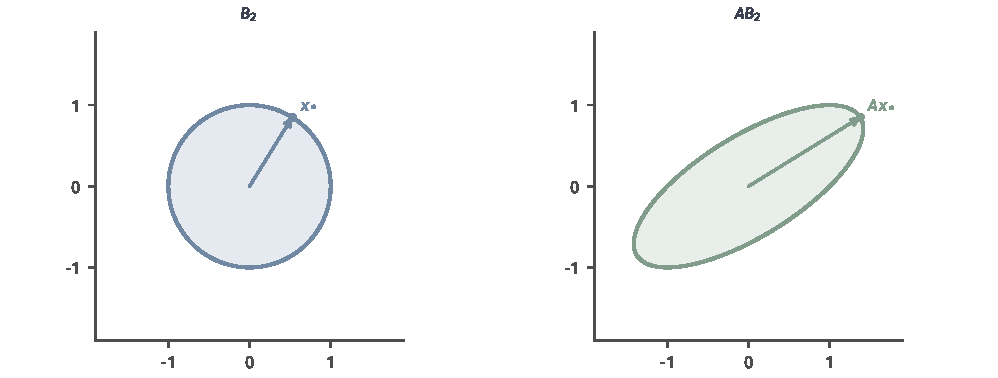
\includegraphics[width=169mm]{figures/00-shared/mathematical-preliminaries-upper/02-linear-spaces/matplotlib/ls-induced-norm-action/ls-induced-norm-action.pdf}
  \caption{诱导矩阵范数衡量最坏放大倍数。左：单位圆$\lVert\bm x\rVert_2=1$；中：线性作用$\bm A$把单位圆映成椭圆；右：椭圆最长的半轴长度就是$\lVert\bm A\rVert_2$，箭头指示最大放大方向。数值由$\bm A$的教学构造直接得到，是解析例。}
  \label{fig:ls-induced-norm-action}
\end{figure*}

\subsubsection{矩阵范数的性质}

有限性与可达性已由定理~\ref{thm:ls-linear-map-continuity}得到。本小节依次求出具体公式、核对范数公理，再给出乘积的上界；这些显式估计用于计算实际的误差常数。

\paragraph{列和与行和公式}
第一式按列计算：
\[
 \lVert\bm A\bm x\rVert_1=\Bigl\lVert\sum_jx_j\bm A_{:,j}\Bigr\rVert_1\leq\sum_j|x_j|\,\lVert\bm A_{:,j}\rVert_1\leq\Bigl(\max_j\lVert\bm A_{:,j}\rVert_1\Bigr)\lVert\bm x\rVert_1.
\]
取$\bm x$为最大绝对列和所在列对应的标准坐标向量时，等号成立。第二式按行计算：对每个$i$，
\[
 |(\bm A\bm x)_i|\leq\sum_j|a_{i,j}|\,|x_j|\leq\Bigl(\sum_j|a_{i,j}|\Bigr)\lVert\bm x\rVert_\infty,
\]
对$i$取最大值即得上界。取输入各坐标为最大绝对行和那一行元素的符号（元素为零处取$1$），等号成立。

\paragraph{谱范数不超过Frobenius范数}
谱范数需要奇异值才能精确计算，但Frobenius范数给出一个容易计算的上界：
\[
 \begin{gathered}
 \lVert\bm A\bm x\rVert_2\leq\lVert\bm A\rVert_{\mathrm F}\lVert\bm x\rVert_2,\\
 \lVert\bm A\rVert_2\leq\lVert\bm A\rVert_{\mathrm F}.
 \end{gathered}
\]
对每行用$p=q=2$的Hölder不等式，得$(\bm A\bm x)_i^2=(\bm A_{i,:}\bm x)^2\leq\lVert\bm A_{i,:}\rVert_2^2\lVert\bm x\rVert_2^2$。对$i$求和，右侧的$\sum_i\lVert\bm A_{i,:}\rVert_2^2$正是$\lVert\bm A\rVert_{\mathrm F}^2$，于是得到第一式。第一式说明每个比值$\lVert\bm A\bm x\rVert_2/\lVert\bm x\rVert_2$都不超过$\lVert\bm A\rVert_{\mathrm F}$，由此得到第二式。

\paragraph{诱导范数是范数}
诱导范数满足范数的各条要求。非负性与齐次性由定义直接得到。若$\lVert\bm A\rVert_{\alpha\to\beta}=0$，则每个$\bm A\bm e_j=\bm0$，即$\bm A=\bm0$，这给出正定性。三角不等式来自$\lVert(\bm A+\bm B)\bm x\rVert_\beta\leq\lVert\bm A\bm x\rVert_\beta+\lVert\bm B\bm x\rVert_\beta$，两边除以$\lVert\bm x\rVert_\alpha$再取上确界即得。

\paragraph{次乘性}
诱导范数还能控制乘积。中间范数匹配时，
\[
 \lVert\bm A\bm B\rVert_{\alpha\to\gamma}
 \leq\lVert\bm A\rVert_{\beta\to\gamma}
 \lVert\bm B\rVert_{\alpha\to\beta}.
\]
这只需连续应用两次诱导范数的界：
\[
 \lVert\bm A\bm B\bm x\rVert_\gamma\leq\lVert\bm A\rVert_{\beta\to\gamma}\lVert\bm B\bm x\rVert_\beta\leq\lVert\bm A\rVert_{\beta\to\gamma}\lVert\bm B\rVert_{\alpha\to\beta}\lVert\bm x\rVert_\alpha.
\]
两边除以$\lVert\bm x\rVert_\alpha$再取上确界即得。反复使用可得$\lVert\bm A^k\rVert_p\leq\lVert\bm A\rVert_p^k$。

\paragraph{Frobenius范数与谱范数的混合界}
乘积的Frobenius范数可以用一个因子的谱范数和另一个因子的Frobenius范数控制：
\begin{equation}
\begin{gathered}
\lVert\bm A\bm B\rVert_{\mathrm F}
 \leq\lVert\bm A\rVert_2\lVert\bm B\rVert_{\mathrm F},\\
\lVert\bm A\bm B\rVert_{\mathrm F}
 \leq\lVert\bm A\rVert_{\mathrm F}\lVert\bm B\rVert_2.
\end{gathered}
\label{eq:matrix-analysis-mixed-submultiplicativity}
\end{equation}
第一式按列计算：
\[
 \lVert\bm A\bm B\rVert_{\mathrm F}^2=\sum_j\lVert\bm A\bm B_{:,j}\rVert_2^2\leq\lVert\bm A\rVert_2^2\sum_j\lVert\bm B_{:,j}\rVert_2^2=\lVert\bm A\rVert_2^2\lVert\bm B\rVert_{\mathrm F}^2.
\]
第二式对转置应用第一式：$\lVert\bm A\bm B\rVert_{\mathrm F}=\lVert\bm B^\top\bm A^\top\rVert_{\mathrm F}\leq\lVert\bm B^\top\rVert_2\lVert\bm A^\top\rVert_{\mathrm F}$。转置不改变Frobenius范数，还需要说明$\lVert\bm B^\top\rVert_2=\lVert\bm B\rVert_2$。对固定的$\bm x$，由$p=q=2$的Hölder不等式，$\lVert\bm y\rVert_2=1$时$|\bm y^\top\bm B\bm x|\leq\lVert\bm B\bm x\rVert_2$；$\bm B\bm x\neq\bm0$时取$\bm y=\bm B\bm x/\lVert\bm B\bm x\rVert_2$即取等号。所以
\[
 \lVert\bm B\rVert_2=\sup_{\lVert\bm x\rVert_2=\lVert\bm y\rVert_2=1}|\bm y^\top\bm B\bm x|.
\]
由于$\bm y^\top\bm B\bm x=\bm x^\top\bm B^\top\bm y$，交换$\bm x,\bm y$的角色，同一个上确界也等于$\lVert\bm B^\top\rVert_2$。再结合$\lVert\bm A\rVert_2\leq\lVert\bm A\rVert_{\mathrm F}$，可知Frobenius范数也满足次乘性：$\lVert\bm A\bm B\rVert_{\mathrm F}\leq\lVert\bm A\rVert_{\mathrm F}\lVert\bm B\rVert_{\mathrm F}$。

\subsection{对偶范数}
\label{sec:ls-dual-norms}

第~\ref{sec:ls-dual-spaces}节的线性泛函是对向量的读取。有了范数，就可以衡量一个读取有多大。误差分析中的典型问题是：误差$\bm r$只知道落在某个范数球内，一次加权读取$\bm z^\top\bm r$最多变化多少。在$\mathbb R^d$上取定一种范数后，这个最大值就是对偶范数。
\begin{definition}[对偶范数]
\label{def:linear-algebra-dual-norm}
给定$\mathbb R^d$上的范数，相对于标准坐标配对的\term{对偶范数}（dual norm）为
\begin{equation}
 \lVert\bm z\rVert_*=\sup_{\lVert\bm r\rVert\leq1}|\bm z^\top\bm r|.
 \label{eq:linear-algebra-dual-norm-definition}
\end{equation}
\end{definition}
这就是上一小节取输出空间为$\mathbb R$时的诱导范数：读取$\bm r\mapsto\bm z^\top\bm r$是$1\times d$矩阵$\bm z^\top$的作用。所以对任意范数，上确界有限并且可以取到。

对偶范数满足范数的各条要求，因而是对偶空间上的范数。非负性显然。$\bm z\neq\bm0$时，取$\bm z$的某个非零坐标$z_j$，则$\bm r=\bm e_j/\lVert\bm e_j\rVert$给出$|\bm z^\top\bm r|=|z_j|/\lVert\bm e_j\rVert>0$，这给出正定性。对每个$\bm r$都有$|(\bm z+\bm w)^\top\bm r|\leq|\bm z^\top\bm r|+|\bm w^\top\bm r|$，取上确界即得三角不等式；齐次性由$|(c\bm z)^\top\bm r|=|c|\,|\bm z^\top\bm r|$得到。图~\ref{fig:ls-dual-norm-unit-ball}把这个最大值画成支撑线最后接触单位球的位置。

\begin{figure}[!htb]
  \centering
  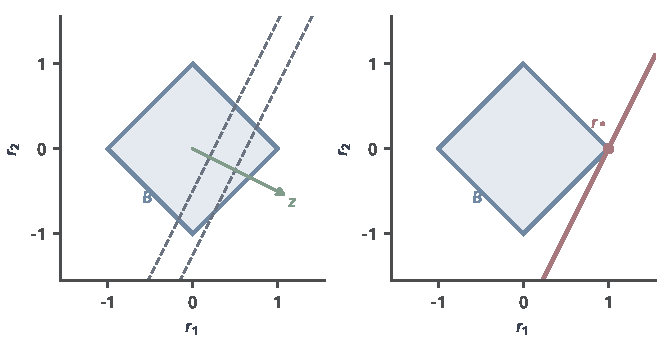
\includegraphics[width=112mm]{figures/00-shared/mathematical-preliminaries-upper/02-linear-spaces/matplotlib/ls-dual-norm-unit-ball/ls-dual-norm-unit-ball.pdf}
  \caption{对偶范数的几何：在原范数单位球$\lVert\bm r\rVert\leq1$上求线性读取$\bm z^\top\bm r$的最大值。左：原单位球（灰色）与读取方向$\bm z$；右：支撑直线最后接触单位球处给出$\lVert\bm z\rVert_*=\max_{\lVert\bm r\rVert\leq1}|\bm z^\top\bm r|$。对偶单位球（虚线）与原单位球互为极体。解析教学例。}
  \label{fig:ls-dual-norm-unit-ball}
\end{figure}

对$\ell_p$范数，对偶范数可以明确写出：
\begin{equation}
(\lVert\cdot\rVert_p)_*=\lVert\cdot\rVert_q,\qquad\frac1p+\frac1q=1.
\label{eq:linear-algebra-lp-duality}
\end{equation}
由齐次性，对任意预算$\rho\geq0$还有
\begin{equation}
 \max_{\lVert\bm r\rVert_p\leq\rho}|\bm z^\top\bm r|
 =\rho\lVert\bm z\rVert_q.
 \label{eq:linear-algebra-linear-perturbation-duality}
\end{equation}
Hölder不等式（定理~\ref{thm:linear-algebra-holder}）给出$\ell_p$单位球上的上界$\lVert\bm z\rVert_q$。这个上界可以达到。$1<p<\infty$且$\bm z\neq\bm0$时，取$r_j=|z_j|^{q-1}\operatorname{sgn}(z_j)/\lVert\bm z\rVert_q^{q-1}$；$\bm z=\bm0$时上界为零，任取可行输入即可。$p=1$时，把单位预算全部放在$|z_j|$最大的坐标上；$p=\infty$时，逐坐标取$r_j=\operatorname{sgn}(z_j)$。下面固定一个读取，比较三种误差预算。
\begin{example}[同一读取在三种误差预算下的最大变化]
\label{ex:ls-dual-norm-three-budgets}
取读取方向$\bm z=(2,-1)^\top$，即读取$\bm z^\top\bm r=2r_1-r_2$，让误差$\bm r$分别落在三种单位球内。

在$\ell_1$单位球上，预算只能分给各坐标的绝对值，全部放在权重$|z_j|$最大的第一个坐标最划算：$\bm r=(1,0)^\top$给出最大值$\lVert\bm z\rVert_\infty=2$。在$\ell_2$单位球上，最坏误差与$\bm z$同方向，取$\bm r=\bm z/\lVert\bm z\rVert_2=(2,-1)^\top/\sqrt5$，最大值为$\lVert\bm z\rVert_2=\sqrt5$。在$\ell_\infty$单位球上，每个坐标都可以同时取满，只需让符号与$z_j$一致：$\bm r=(1,-1)^\top$给出最大值$\lVert\bm z\rVert_1=3$。换成实际的误差预算$|r_j|\leq0.01$，就在式~\eqref{eq:linear-algebra-linear-perturbation-duality}中取$p=\infty$、$\rho=0.01$，最大变化为$0.01\cdot(2+1)=0.03$，由$\bm r=(0.01,-0.01)^\top$达到。

三种单位球给出的最大值依次为$2$、$\sqrt5$、$3$。读取本身没有变，变的是允许误差的形状：它决定了最坏方向在哪里，也决定了读取方向要用哪个对偶范数计量。
\end{example}
图~\ref{fig:linear-algebra-dual-unit-balls}画出这三种情形下的最坏方向。
\begin{figure*}[htbp]
  \centering
  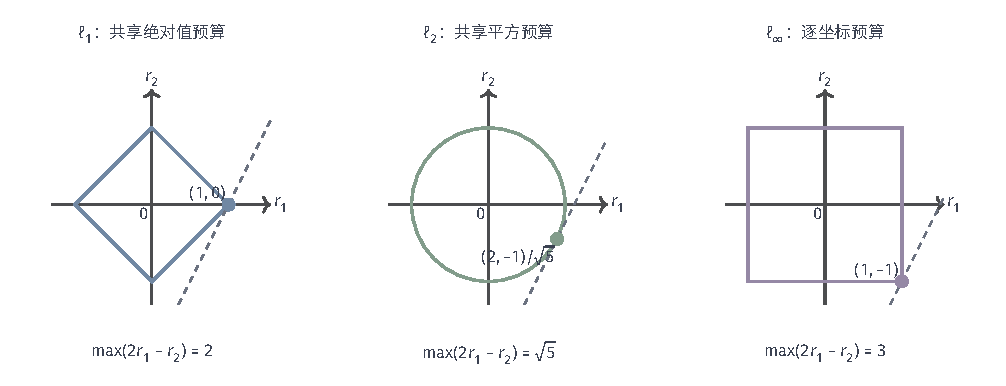
\includegraphics[width=168.998mm]{figures/00-shared/mathematical-preliminaries-upper/02-linear-spaces/tikz/linear-algebra-dual-unit-balls/figure.pdf}
  \caption{同一线性读取$2r_1-r_2$在$\ell_1$、$\ell_2$、$\ell_\infty$单位球上的最大值依次为$2$、$\sqrt5$、$3$。虚线为最后接触可行集的支撑直线，点为最大化方向。三图坐标尺度相同，均为解析教学例；允许误差的形状改变时，误差常数也随之改变。}
  \label{fig:linear-algebra-dual-unit-balls}
\end{figure*}

由此可见，误差预算按$\ell_\infty$给出时，读取方向要按$\ell_1$计量；预算按$\ell_2$给出时，读取方向仍按$\ell_2$计量。

原空间的范数改变，对偶范数随之改变。对加权的坐标范数，可以用换元把问题化回已知情形。
\begin{example}[加权$\ell_1$范数的对偶范数]
\label{ex:ls-weighted-dual-norm}
设权重$w_1,\ldots,w_d>0$，在$\mathbb R^d$上取加权范数$\lVert\bm r\rVert_{\bm w}=\sum_jw_j|r_j|$。把权重吸收进变量，令$s_j=w_jr_j$，则$\lVert\bm r\rVert_{\bm w}=\lVert\bm s\rVert_1$，$\bm z^\top\bm r=\sum_j(z_j/w_j)s_j$。$\bm r$取遍$\lVert\bm r\rVert_{\bm w}\leq1$时，$\bm s$恰好取遍$\ell_1$单位球。由式~\eqref{eq:linear-algebra-lp-duality}中$p=1$的情形，
\[
 \lVert\bm z\rVert_*=\max_j\frac{|z_j|}{w_j}.
\]
仍取上例的$\bm z=(2,-1)^\top$。不加权，即$\bm w=(1,1)^\top$时，$\lVert\bm z\rVert_*=2$，由$\bm r=(1,0)^\top$取到，与上例的$\ell_1$情形一致；改用$\bm w=(4,1)^\top$时，$\lVert\bm z\rVert_*=\max\{1/2,1\}=1$，由$\bm r=(0,-1)^\top$取到。

读取$\bm z^\top\bm r$的代数表达没有变，它的大小却随原空间的范数改变。第一个坐标的权重变大后，同样的预算只允许它有更小的变化，最坏方向因而转到第二个坐标。
\end{example}
所以讨论“输入误差最多引起多大输出误差”时，必须先说清误差用哪种范数度量。内积诱导的范数下，对偶范数等于表示向量的长度，在第~\ref{sec:ls-riesz-representation}节证明。一般有限维空间$V$上的线性泛函$\varphi$同样定义$\lVert\varphi\rVert_*=\max_{\lVert\bm v\rVert\leq1}|\varphi(\bm v)|$，它是取$W=\mathbb R$时的算子范数。无限维空间中，并非每个线性泛函都连续，代数对偶与连续对偶需要区分，这同样属于无限维理论。

\subsection{商范数}
\label{sec:ls-quotient-norms}

子空间的闭性还可以用来给商空间定义范数。第~\ref{sec:ls-quotient-spaces}节的商空间$V/U$把相差$U$中向量的点看成同一个类$\bm x+U$，那里只建立了线性结构。要度量一个类的大小，自然的选择是类中的点到$U$的距离。这个距离不依赖类中代表元的选取：若$\bm x'=\bm x+\bm u_0$，$\bm u_0\in U$，则$\bm u$遍历$U$时$\bm u-\bm u_0$也遍历$U$，所以$d(\bm x',U)=d(\bm x,U)$。于是可以定义\term{商范数}（quotient norm）
\[
 \lVert\bm x+U\rVert_{V/U}=d(\bm x,U)=\inf_{\bm u\in U}\lVert\bm x-\bm u\rVert .
\]

它满足范数的三条要求。三角不等式：对任意$\bm u,\bm u'\in U$，
\[
 d(\bm x+\bm y,U)\leq\lVert(\bm x-\bm u)+(\bm y-\bm u')\rVert\leq\lVert\bm x-\bm u\rVert+\lVert\bm y-\bm u'\rVert;
\]
取$\bm u,\bm u'$使右侧两项分别任意接近$d(\bm x,U)$与$d(\bm y,U)$，即得$d(\bm x+\bm y,U)\leq d(\bm x,U)+d(\bm y,U)$。齐次性：$c\neq0$时$cU=U$，所以$d(c\bm x,U)=|c|\,d(\bm x,U)$；$c=0$时两边都为零。正定性要求$d(\bm x,U)=0$只在$\bm x+U=U$即$\bm x\in U$时发生，这正是前面由子空间闭性得到的结论。在子空间不一定闭的更一般空间中，同一个公式可能只给出半范数，有限维的结论不能无条件外推。

\paragraph{一般范数下的最近点}
商范数是一个下确界。这个下确界能否取到，就是$U$中是否存在离给定点最近的点。
\begin{theorem}[最近点的存在]
\label{thm:multivariable-nearest-point-existence}
设$V$是有限维赋范空间，$U$是子空间，$\bm x\in V$，则存在$\bm u^\star\in U$，使$\lVert\bm x-\bm u^\star\rVert=d(\bm x,U)$。
\end{theorem}
\begin{proof}
在$U$中取$\bm u_k$，使$\lVert\bm x-\bm u_k\rVert\to d(\bm x,U)$。由$\lVert\bm u_k\rVert\leq\lVert\bm x\rVert+\lVert\bm x-\bm u_k\rVert$，序列$(\bm u_k)$有界。由定理~\ref{thm:multivariable-bolzano-weierstrass}（范数等价使它对任意范数适用），存在收敛子列$\bm u_{k_i}\to\bm u^\star$；由子空间闭性，$\bm u^\star\in U$。范数连续，所以$\lVert\bm x-\bm u^\star\rVert=\lim_i\lVert\bm x-\bm u_{k_i}\rVert=d(\bm x,U)$。
\end{proof}
最近点存在，却可能不唯一。
\begin{example}[反例：$\ell_\infty$范数下最近点不唯一]
\label{ex:ls-linf-nonunique-nearest}
在$\mathbb R^2$上取$\ell_\infty$范数，求点$\bm y=(0,1)^\top$到横轴$U=\operatorname{span}\{(1,0)^\top\}$的最近点。$U$中的点写成$(t,0)^\top$，差向量为$(-t,1)^\top$，于是
\[
 \lVert\bm y-(t,0)^\top\rVert_\infty=\max\{|t|,1\}\geq1,
\]
等号当且仅当$|t|\leq1$时成立。

所以$d(\bm y,U)=1$，而且横轴上整整一段$|t|\leq1$的点$(t,0)^\top$都是最近点。原因在于$\ell_\infty$只看最大坐标：竖直方向的差已经是$1$，水平方向的差只要不超过$1$，就不影响距离。欧氏范数下只有$t=0$达到最小距离，可见最近点是否唯一取决于所用的范数，而不只取决于点和子空间。
\end{example}
加入内积以后，第~\ref{sec:ls-orthogonal-projection}节将证明正交投影给出唯一的最近点。一般范数下的存在性与内积几何下的唯一性，回答的是两个不同的问题。


% 内积空间（内积与诱导范数、Gram矩阵）、正交与投影（正交补、标准正交基、Gram--Schmidt正交化、正交投影）、线性泛函的内积表示与伴随。

\section{内积空间}
\label{sec:ls-inner-product-spaces}

范数只度量大小，不给出角度。一般范数下谈不上两个方向是否垂直，向子空间的最近点也可能不唯一（示例~\ref{ex:ls-linf-nonunique-nearest}）。第~\ref{chap:linear-operations}章在$\mathbb R^d$上用逐项相乘再求和定义了欧氏内积，并由它得到长度和夹角。本节提取这种计算的共同规则，在一般线性空间上定义内积。

本节先从内积公理推出长度、夹角和几个基本不等式，再用Gram矩阵记录一组向量的两两内积。正交投影、标准正交基和伴随在随后两节讨论。

\subsection{内积与内积诱导的范数}
\label{sec:ls-inner-product-definition}

本小节先给出内积的公理和例子，再由内积定义长度、正交与夹角，最后从三角不等式出发，说明内积诱导的长度是范数，从而给出距离；平行四边形恒等式则说明，并非每个范数都来自内积。

\subsubsection{内积的定义}
\label{sec:ls-inner-product-axioms}

欧氏内积对每个变量都保持线性组合，交换两个变量不改变结果，向量与自身的内积只在零向量处为零。这些性质只涉及线性运算，因此可以用来定义一般空间上的内积。
\begin{definition}[内积空间]
\label{def:functional-inner-product-space}
\label{def:linear-algebra-inner-product}
设$V$是实线性空间。映射$\langle\cdot,\cdot\rangle:V\times V\to\mathbb R$若对任意$\bm x,\bm y,\bm z\in V$与$a,b\in\mathbb R$满足
\begin{enumerate}
 \item 双线性：$\langle a\bm x+b\bm y,\bm z\rangle=a\langle\bm x,\bm z\rangle+b\langle\bm y,\bm z\rangle$，且$\langle\bm z,a\bm x+b\bm y\rangle=a\langle\bm z,\bm x\rangle+b\langle\bm z,\bm y\rangle$；
 \item 对称性：$\langle\bm x,\bm y\rangle=\langle\bm y,\bm x\rangle$；
 \item 正定性：$\langle\bm x,\bm x\rangle\geq0$，且$\langle\bm x,\bm x\rangle=0$当且仅当$\bm x=\bm0$，
\end{enumerate}
就称为$V$上的\term{内积}（inner product）；配备内积的线性空间$(V,\langle\cdot,\cdot\rangle)$称为\term{内积空间}（inner-product space）。
\end{definition}

\paragraph{内积的例子}
先检验欧氏内积满足这三条公理。设$\bm x,\bm y,\bm z\in\mathbb R^d$，$a,b\in\mathbb R$。对称性成立，因为每一项$x_jy_j=y_jx_j$。对第一个变量的线性来自有限和的运算法则：
\[
 \sum_j(ax_j+bz_j)y_j=a\sum_jx_jy_j+b\sum_jz_jy_j,
\]
再由对称性，对第二个变量同样成立。正定性成立，因为$\langle\bm x,\bm x\rangle=\sum_jx_j^2\geq0$，而非负数之和为零时每一项都为零。

同形矩阵上的Frobenius内积也满足三条公理。它对两个变量分别线性；交换两个矩阵不改变各项乘积，因而对称；$\langle\bm A,\bm A\rangle_{\mathrm F}=\sum_{i,j}a_{i,j}^2$非负，并且只在$\bm A=\bm0$时为零。这正是把$mn$个元素看作坐标时欧氏内积的三条性质。所以下面从公理推出的一般结论对它同样成立。

标准内积之外，一般空间上还可以有各种内积。下面在$P_1$上规定一个只看两点取值的内积，后面的算例会反复用到它。
\begin{example}[只看两点取值的内积]
\label{ex:ls-two-point-inner-product}
在$P_1$上规定
\[
 \langle f,g\rangle=f(0)g(0)+f(1)g(1),
\]
即把两个函数在$t=0,1$处的取值配对相乘再相加。函数值$f(0)$、$f(1)$都随$f$线性变化，所以右端对$f$与对$g$分别线性；交换$f,g$不改变右端，对称性也成立。正定性要用到$P_1$的特点：$\langle f,f\rangle=f(0)^2+f(1)^2\geq0$，若它为零，则$f(0)=f(1)=0$；对$f=a+bt$，这就是$a=0$、$a+b=0$，故$f=0$。一次多项式由两个点的取值确定，这一步才能成立。

因此这一规则是$P_1$上的内积。它与系数向量$(a,b)^\top$的欧氏内积并不相同：例如$\langle1,t\rangle=1\cdot0+1\cdot1=1$，而$1$与$t$的系数向量$(1,0)^\top$、$(0,1)^\top$的欧氏内积为零。同一对函数是否正交，要看采用哪种内积。
\end{example}

\paragraph{复内积的约定}
上面的定义针对实空间。在复空间中，若两个变量都按复数线性，并且满足实数式的对称性，那么$\langle\mathrm i\bm x,\mathrm i\bm x\rangle=-\langle\bm x,\bm x\rangle$，无法对非零向量保持正定。因此复内积采用另一种约定：对第一个变量共轭线性，对第二个变量线性，并满足$\langle\bm x,\bm y\rangle=\overline{\langle\bm y,\bm x\rangle}$。标准例子是$\langle\bm x,\bm y\rangle=\bm x^*\bm y$，其中$\bm x^*$表示共轭转置；仍要求$\langle\bm x,\bm x\rangle>0$对非零$\bm x$成立。

后面的Cauchy--Schwarz不等式在复内积下同样成立。若$\bm y\ne\bm0$，在$\lVert\bm x-\alpha\bm y\rVert^2\geq0$中取$\alpha=\langle\bm y,\bm x\rangle/\lVert\bm y\rVert^2$，展开可得$|\langle\bm x,\bm y\rangle|^2\leq\lVert\bm x\rVert^2\lVert\bm y\rVert^2$。因此它的平方根仍给出范数。但复内积的值可能不是实数，下一小节用余弦定义夹角的公式不能直接照搬。下文的证明继续使用实内积，复情形需要把转置相应改为共轭转置。

\subsubsection{由内积定义的夹角}
\label{sec:ls-inner-product-angle}

\paragraph{长度与正交}
与$\mathbb R^d$中一样，内积给出长度$\lVert\bm v\rVert=\sqrt{\langle\bm v,\bm v\rangle}$，它是否满足范数的全部要求，留到下一小节检验；$\langle\bm x,\bm y\rangle=0$时称$\bm x,\bm y$正交。正交的两个向量满足勾股定理。展开
\[
 \lVert\bm x+\bm y\rVert^2=\lVert\bm x\rVert^2+2\langle\bm x,\bm y\rangle+\lVert\bm y\rVert^2,
\]
交叉项为零，得$\lVert\bm x+\bm y\rVert^2=\lVert\bm x\rVert^2+\lVert\bm y\rVert^2$。

\paragraph{Cauchy--Schwarz不等式}
平面上两个非零向量的夹角$\theta$满足
\[
 \langle\bm x,\bm y\rangle=\lVert\bm x\rVert\,\lVert\bm y\rVert\cos\theta.
\]
要在一般内积空间中反过来用这个关系定义夹角，须先保证内积除以两个长度之积后总落在$[-1,1]$中。下面的不等式给出这一保证。
\begin{theorem}[Cauchy--Schwarz不等式]
\label{thm:linear-algebra-cauchy-schwarz}
对任一内积及其长度，任意向量$\bm x,\bm y$满足
\begin{equation}
 |\langle\bm x,\bm y\rangle|\leq\lVert\bm x\rVert\,\lVert\bm y\rVert,
 \label{eq:prelim-cauchy-schwarz}
\end{equation}
等号成立当且仅当其中一个向量是另一个向量的实数倍。
\end{theorem}
\begin{proof}
$\bm y=\bm0$时两边都为零。设$\bm y\neq\bm0$。对任意实数$s$，向量$\bm x-s\bm y$的长度平方非负；按内积的对称性与双线性展开，
\[
 0\leq\lVert\bm x-s\bm y\rVert^2
 =\lVert\bm x\rVert^2-2s\langle\bm x,\bm y\rangle+s^2\lVert\bm y\rVert^2.
\]
右侧是$s$的二次函数，二次项系数为正，在顶点$s=\langle\bm x,\bm y\rangle/\lVert\bm y\rVert^2$处最小，最小值为$\lVert\bm x\rVert^2-\langle\bm x,\bm y\rangle^2/\lVert\bm y\rVert^2$。它非负，两边乘以$\lVert\bm y\rVert^2$再开平方，即得不等式。等号成立当且仅当对这个$s$有$\bm x-s\bm y=\bm0$，即$\bm x$是$\bm y$的实数倍；连同$\bm y=\bm0$的情形，即得等号条件。
\end{proof}
证明只用了内积的三条公理，所以不等式对每一种内积都成立。在$\mathbb R^d$的标准内积下，它就是$p=q=2$的Hölder不等式（定理~\ref{thm:linear-algebra-holder}）；对Frobenius内积，它给出$|\langle\bm A,\bm B\rangle_{\mathrm F}|\leq\lVert\bm A\rVert_{\mathrm F}\lVert\bm B\rVert_{\mathrm F}$。

\paragraph{夹角}
由Cauchy--Schwarz不等式，非零向量的夹角$\theta\in[0,\pi]$可以由
\[
 \cos\theta=\frac{\langle\bm x,\bm y\rangle}{\lVert\bm x\rVert\,\lVert\bm y\rVert}
 =\left\langle\frac{\bm x}{\lVert\bm x\rVert},\frac{\bm y}{\lVert\bm y\rVert}\right\rangle
\]
定义。第二种写法说明，夹角只比较方向：先把两个向量各自归一化为单位向量，再取内积，所以$\bm x$与$c\bm x$（$c>0$）给出同一个方向。正交恰好对应$\theta=\pi/2$，这就是把正交称为垂直的理由。由等号条件，$\cos\theta=\pm1$恰好对应两个向量共线。分子和分母必须来自同一个内积；一边用$\ell_2$、一边用$\ell_1$计量长度时，这个比值没有几何意义。

回到第~\ref{chap:linear-operations}章贯穿例中两个特征的取值向量，计算它们的夹角。
\begin{example}[贯穿例两列的夹角]
\label{ex:ls-nearly-collinear-angle}
贯穿例的两列是$\bm c_1=(1,1,1)^\top$与$\bm c_2=(1,1+\varepsilon,1-\varepsilon)^\top$，取欧氏内积。夹角公式需要一个内积和两个长度：$\langle\bm c_1,\bm c_2\rangle=1+(1+\varepsilon)+(1-\varepsilon)=3$，其中$\pm\varepsilon$恰好抵消；$\lVert\bm c_1\rVert_2^2=3$；$\lVert\bm c_2\rVert_2^2=1+(1+\varepsilon)^2+(1-\varepsilon)^2=3+2\varepsilon^2$，一次项同样抵消，只剩下二次项。所以
\begin{equation}
 \cos\theta_\varepsilon=\frac{3}{\sqrt3\,\sqrt{3+2\varepsilon^2}}
 =\frac{1}{\sqrt{1+2\varepsilon^2/3}}\longrightarrow1\qquad(\varepsilon\to0).
 \label{eq:linear-algebra-nearly-collinear-angle}
\end{equation}
代入具体数值：$\varepsilon=0.1$时$\cos\theta_\varepsilon\approx0.9967$，夹角约$4.7^\circ$；$\varepsilon=0.01$时$\cos\theta_\varepsilon\approx0.99997$，夹角不到$0.5^\circ$。

可见$\varepsilon\to0$时两列的夹角趋于零。$\varepsilon$非零时两个向量并不重合，但$\varepsilon$很小时它们几乎同向：$\varepsilon$只以平方出现在余弦中，余弦与$1$只差$\varepsilon^2$量级。
\end{example}
两个向量不重合却几乎同向，称为\term{近共线}（nearly collinear）。这里的“近”指两列作为$\mathbb R^3$中向量的夹角很小，不是说各个样本点彼此接近。夹角也依赖所用的内积：换一种内积，同样两个向量的夹角会改变。

\subsubsection{由内积定义的距离}
\label{sec:ls-inner-product-distance}

\paragraph{三角不等式}
有了长度，自然想用$\lVert\bm x-\bm y\rVert$度量两个向量的距离。这要求长度是一个范数，其中关键是三角不等式：从$\bm x$到$\bm z$的距离不超过经过$\bm y$绕行的距离。定义~\ref{def:ls-normed-space}的正定性直接来自内积的正定性，齐次性来自$\langle c\bm x,c\bm x\rangle=c^2\langle\bm x,\bm x\rangle$。需要证明的是三角不等式，而Cauchy--Schwarz不等式正好控制展开式中的交叉项。
\begin{theorem}[内积诱导长度的三角不等式]
\label{thm:ls-inner-product-triangle}
设$V$是内积空间，$\lVert\bm v\rVert=\sqrt{\langle\bm v,\bm v\rangle}$，则对任意$\bm x,\bm y\in V$，
\[
 \lVert\bm x+\bm y\rVert\leq\lVert\bm x\rVert+\lVert\bm y\rVert,
\]
等号成立当且仅当其中一个向量是另一个向量的非负实数倍。
\end{theorem}
\begin{proof}
按双线性与对称性展开平方，再对交叉项用$\langle\bm x,\bm y\rangle\leq|\langle\bm x,\bm y\rangle|$与Cauchy--Schwarz不等式~\eqref{eq:prelim-cauchy-schwarz}：
\[
 \begin{aligned}
 \lVert\bm x+\bm y\rVert^2
 &=\lVert\bm x\rVert^2+2\langle\bm x,\bm y\rangle+\lVert\bm y\rVert^2\\
 &\leq\lVert\bm x\rVert^2+2\lVert\bm x\rVert\lVert\bm y\rVert+\lVert\bm y\rVert^2\\
 &=(\lVert\bm x\rVert+\lVert\bm y\rVert)^2.
 \end{aligned}
\]
两边都非负，开平方即得不等式。等号成立当且仅当$\langle\bm x,\bm y\rangle=\lVert\bm x\rVert\,\lVert\bm y\rVert$。若$\bm y=\bm0$，结论显然。若$\bm y\neq\bm0$，由Cauchy--Schwarz不等式的等号条件，$\bm x=s\bm y$；代入得$s\lVert\bm y\rVert^2=|s|\,\lVert\bm y\rVert^2$，即$s\geq0$。反过来，$\bm x=s\bm y$且$s\geq0$时，两侧都等于$(1+s)\lVert\bm y\rVert$。
\end{proof}

\paragraph{内积诱导的范数与距离}
由定理~\ref{thm:ls-inner-product-triangle}，长度$\lVert\bm v\rVert=\sqrt{\langle\bm v,\bm v\rangle}$满足范数的三条要求，称为内积\emph{诱导的范数}。它给出距离
\[
 d(\bm x,\bm y)=\lVert\bm x-\bm y\rVert=\sqrt{\langle\bm x-\bm y,\bm x-\bm y\rangle},
\]
欧氏距离与Frobenius距离都是这样得到的。于是每个内积空间都是赋范空间，前三节关于范数、收敛与完备性的结论都适用于它。与一般范数相比，这个距离还可以用内积展开：$\lVert\bm x-\bm y\rVert^2=\lVert\bm x\rVert^2-2\langle\bm x,\bm y\rangle+\lVert\bm y\rVert^2$，距离的平方由两个长度与夹角决定，这正是余弦定理。下面的平行四边形恒等式说明，这一额外结构可以用来区分哪些范数来自内积。

\paragraph{平行四边形恒等式}
反过来，并非每个范数都由内积给出。内积诱导的范数还满足一条额外的等式，即\term{平行四边形恒等式}。几何上，它表示平行四边形两条对角线长度的平方和等于四条边长度的平方和。
\begin{theorem}[平行四边形恒等式]
\label{thm:linear-algebra-parallelogram}
设$V$是实内积空间，$\bm x,\bm y\in V$，以该内积诱导的范数计量长度，则
\begin{equation}
 \lVert\bm x+\bm y\rVert^2+\lVert\bm x-\bm y\rVert^2
 =2\lVert\bm x\rVert^2+2\lVert\bm y\rVert^2.
 \label{eq:functional-parallelogram-identity}
\end{equation}
欧氏范数是这一结论的特例。
\end{theorem}
\begin{proof}
记$\lVert\bm u\rVert^2=\langle\bm u,\bm u\rangle$。由内积的双线性和对称性，分别展开和向量与差向量的长度平方：
\[
 \begin{aligned}
 \lVert\bm x+\bm y\rVert^2
 &=\lVert\bm x\rVert^2+2\langle\bm x,\bm y\rangle+\lVert\bm y\rVert^2,\\
 \lVert\bm x-\bm y\rVert^2
 &=\lVert\bm x\rVert^2-2\langle\bm x,\bm y\rangle+\lVert\bm y\rVert^2.
 \end{aligned}
\]
两式相加，交叉项相互抵消，得到所需恒等式。证明只用了内积公理，因此适用于定义~\ref{def:linear-algebra-inner-product}中的任一实内积。
\end{proof}

这条恒等式可以用来检验一个范数是否来自内积：只要某个范数在一对向量上使恒等式两侧不等，它就不可能由任何内积给出。下面用这个办法检验$\ell_1$与$\ell_\infty$范数。
\begin{example}[反例：$\ell_1$与$\ell_\infty$范数不来自内积]
\label{ex:ls-l1-linf-not-inner-product}
取$\mathbb R^2$中的两个标准坐标向量$\bm x=\bm e_1$、$\bm y=\bm e_2$作为平行四边形的两条边，两条对角线分别是$\bm x+\bm y=(1,1)^\top$与$\bm x-\bm y=(1,-1)^\top$。在$\ell_1$、$\ell_2$、$\ell_\infty$范数下，四条边的长度都是$1$，差别出在对角线上。对$\ell_1$范数，两条对角线都长$2$：
\[
 \begin{gathered}
 \lVert\bm x+\bm y\rVert_1^2+\lVert\bm x-\bm y\rVert_1^2=2^2+2^2=8,\\
 2\lVert\bm x\rVert_1^2+2\lVert\bm y\rVert_1^2=2\cdot1^2+2\cdot1^2=4;
 \end{gathered}
\]
对$\ell_\infty$范数，两条对角线都只长$1$：
\[
 \begin{gathered}
 \lVert\bm x+\bm y\rVert_\infty^2+\lVert\bm x-\bm y\rVert_\infty^2=1^2+1^2=2,\\
 2\lVert\bm x\rVert_\infty^2+2\lVert\bm y\rVert_\infty^2=4.
 \end{gathered}
\]
$\ell_1$范数使左侧偏大，$\ell_\infty$范数使左侧偏小，恒等式都不成立。所以不存在内积使$\lVert\bm x\rVert_1=\sqrt{\langle\bm x,\bm x\rangle}$对一切$\bm x$成立；$\ell_\infty$范数同样不是由内积给出的长度。作为对照，欧氏范数下两条对角线长都是$\sqrt2$，左侧为$4$，与右侧相等。
\end{example}
因此一般范数只能度量大小，不能用上面的公式定义夹角。

另一方面，内积可以由它诱导的范数恢复。在实空间中，分别展开$\lVert\bm x+\bm y\rVert^2$与$\lVert\bm x-\bm y\rVert^2$并相减，得到极化恒等式
\[
 \langle\bm x,\bm y\rangle=\frac14\bigl(\lVert\bm x+\bm y\rVert^2-\lVert\bm x-\bm y\rVert^2\bigr).
\]
所以两个实内积若给出同一个范数，就必相同。

\paragraph{Hilbert空间}
\label{sec:ls-hilbert-spaces}
内积诱导的范数使内积空间成为赋范空间。若这个范数下的每个柯西列都收敛到空间内的元素，就称它为\term{Hilbert空间}（Hilbert space，也译作希尔伯特空间）。

由定理~\ref{thm:ls-finite-dimensional-complete}，有限维内积空间都是Hilbert空间。后面的正交分解与正交投影都用有限维的代数构造得到，不依赖完备性。无限维空间中，完备性与子空间的闭性都需要另行检查；无限正交级数、闭子空间上的投影以及连续泛函的表示，属于本章开头提到的无限维理论。

\subsection{Gram矩阵}
\label{sec:ls-gram-psd}

一组向量的全部两两内积可以排成一个对称矩阵，即Gram矩阵。本小节先引入正定与半正定矩阵，并用正定矩阵定义$\mathbb R^d$上的加权内积；然后定义Gram矩阵，说明Gram矩阵恰好是全部半正定矩阵，从中可以读出这组向量是否线性无关、是否两两正交。借助这一刻画，可以证明逐元素乘积保持半正定。最后用基的Gram矩阵写出一般内积在坐标下的计算公式。

\subsubsection{正定与半正定}
\label{sec:ls-positive-definite}
$n$阶对称矩阵$\bm M$与向量$\bm x\in\mathbb R^n$给出一个数
\[
 q(\bm x)=\sum_{i=1}^n\sum_{j=1}^n m_{i,j}x_ix_j,
\]
称为$\bm M$的二次型；用矩阵乘法，它写作$\bm x^\top\bm M\bm x$。

若对每个非零$\bm x$都有$q(\bm x)>0$，就称$\bm M$\term{正定}（positive definite），记作$\bm M\succ\bm0$；若只保证$q(\bm x)\geq0$对一切$\bm x$成立，就称$\bm M$\term{半正定}（positive semidefinite），记作$\bm M\succeq\bm0$。

对两个同阶对称矩阵，$\bm M\succeq\bm N$表示$\bm M-\bm N\succeq\bm0$，即$\bm M$的二次型处处不小于$\bm N$的二次型。它比较的是两个二次型，不是逐个元素。

判断正定性，要看二次型能否在某个非零向量处取到零或负值。下面用配方比较两个二阶矩阵。
\begin{example}[用配方区分正定与半正定]
\label{ex:ls-pd-psd-completing-square}
比较
\[
 \bm M=\begin{bmatrix}4&2\\2&2\end{bmatrix},\quad
 \bm N=\begin{bmatrix}1&1\\1&1\end{bmatrix}.
\]
把二次型配成平方和，非负性一目了然，剩下的问题是平方和能否在非零向量处为零：
\[
 \begin{aligned}
 q_{\bm M}(\bm x)&=4x_1^2+4x_1x_2+2x_2^2=(2x_1+x_2)^2+x_2^2,\\
 q_{\bm N}(\bm x)&=x_1^2+2x_1x_2+x_2^2=(x_1+x_2)^2.
 \end{aligned}
\]
$q_{\bm M}$是两个平方之和，只在$2x_1+x_2=0$且$x_2=0$，即$\bm x=\bm0$时为零，所以$\bm M\succ\bm0$。$q_{\bm N}$只有一个平方，它处处非负，却在非零向量$\bm x=(1,-1)^\top$处为零，所以$\bm N\succeq\bm0$而不是正定矩阵。两个变量的二次型配出两个独立的平方项时正定，只配出一个平方项时半正定而不正定。
\end{example}

对角矩阵的情形最简单。它的二次型是$\sum_id_ix_i^2$。若全部$d_i>0$，每个非零$\bm x$都使它为正；若某个$d_i\leq0$，取$\bm x=\bm e_i$就得到$q(\bm e_i)=d_i\leq0$。所以对角矩阵正定当且仅当全部$d_i>0$，例如$\bm I_n\succ\bm0$。

一般矩阵的正定性要对全部非零向量检查，只看元素的符号并不够。
\begin{example}[反例：元素全为正的对称矩阵未必正定]
\label{ex:ls-positive-entries-not-pd}
矩阵
\[
 \bm M=\begin{bmatrix}1&2\\2&1\end{bmatrix}
\]
的四个元素都为正，二次型为$q(\bm x)=x_1^2+4x_1x_2+x_2^2$。交叉项系数比两个平方项大，只要让$x_1,x_2$异号，交叉项就会占上风。取$\bm x=(1,-1)^\top$，
\[
 q(\bm x)=1^2+4\cdot1\cdot(-1)+(-1)^2=-2<0,
\]
所以$\bm M$不是正定矩阵，连半正定也不是。决定正定性的是二次型在所有方向上的取值，而不是元素的符号。
\end{example}

\paragraph{加权内积}
\phantomsection
\label{sec:ls-weighted-inner-products}
正定矩阵可以用来在$\mathbb R^d$上定义标准内积以外的内积。各坐标的单位或重要性不同时，可以给不同方向不同的权重：取对称正定矩阵$\bm M$，规定
\begin{equation}
\begin{gathered}
\langle\bm x,\bm y\rangle_{\bm M}=\bm x^\top\bm M\bm y,\\
d_{\bm M}(\bm x,\bm y)=\lVert\bm x-\bm y\rVert_{\bm M}=\sqrt{(\bm x-\bm y)^\top\bm M(\bm x-\bm y)}.
\end{gathered}
\label{eq:linear-algebra-mahalanobis-pseudodistance}
\end{equation}
双线性来自矩阵乘法的分配律，对称性来自$\bm M^\top=\bm M$，正定性就是$\bm M$的正定性。所以它满足内积的三条公理，称为加权内积，$d_{\bm M}$是它给出的距离。统计中取$\bm M$为协方差矩阵的逆，得到的就是Mahalanobis距离。下面看权重怎样改变同一个点的长度。
\begin{example}[加权内积下的长度]
\label{ex:ls-weighted-length}
取$\bm M=\operatorname{diag}(4,1)$，加权内积就是$\langle\bm x,\bm y\rangle_{\bm M}=4x_1y_1+x_2y_2$，第一个坐标的乘积被计为四倍。对点$\bm x=(1,1)^\top$，$\lVert\bm x\rVert_{\bm M}^2=4\cdot1+1\cdot1=5$，而欧氏长度的平方只有$1+1=2$。同一个点的加权长度是$\sqrt5$，欧氏长度是$\sqrt2$：权重放大了第一个坐标对长度的贡献，第一个坐标上的偏差因而比第二个坐标上同样大小的偏差显得更远。
\end{example}
本小节最后将说明，选定基以后，任一实内积都可以写成这种加权形式。

\subsubsection{Gram矩阵的定义}
\label{sec:ls-gram-orthogonality}
正交是两个向量之间的关系。一组向量$\bm b_1,\ldots,\bm b_r$之间有$r^2$个内积值，把它们排成一个矩阵，就能一次记录这组向量的全部相互关系。
\begin{definition}[有限向量族的Gram矩阵]
\label{def:linear-algebra-gram-matrix}
设$\bm b_1,\ldots,\bm b_r$是内积空间$V$中的向量。以$g_{i,j}=\langle\bm b_i,\bm b_j\rangle$为元素的$r$阶矩阵$\bm G$称为它们的\term{Gram矩阵}（Gram matrix）。在$\mathbb R^m$中，若$\bm B$以这些向量为列，则欧氏内积下$\bm G=\bm B^\top\bm B$，加权内积$\langle\cdot,\cdot\rangle_{\bm M}$下$\bm G=\bm B^\top\bm M\bm B$。
\end{definition}
矩阵形式来自乘积的元素公式：$(\bm B^\top\bm B)_{i,j}$是$\bm B^\top$的第$i$行（即$\bm b_i^\top$）与$\bm B$的第$j$列相乘。由内积的对称性，$\bm G$是对称矩阵。

正交性写在Gram矩阵的非对角元里：$\bm G$是对角矩阵，恰好表示这组向量两两正交；$\bm G=\bm I_r$，则表示它们两两正交且长度都为$1$。图~\ref{fig:ls-gram-matrix-coefficients}把两个向量的两两内积排成数表。
\begin{figure}[!htb]
  \centering
  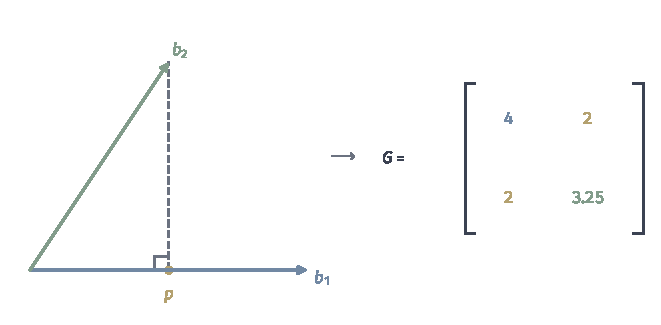
\includegraphics[width=112mm]{figures/00-shared/mathematical-preliminaries-upper/02-linear-spaces/matplotlib/ls-gram-matrix-coefficients/ls-gram-matrix-coefficients.pdf}
  \caption{Gram矩阵把一组基向量的两两内积排成数表。左：平面上两条不垂直的基向量$\bm b_1,\bm b_2$及其夹角；右：$G_{i,j}=\langle\bm b_i,\bm b_j\rangle$构成的$2\times2$Gram矩阵，对角元为各向量长度的平方，非对角元为两向量的内积。基越接近正交，非对角元越接近零；两向量共线时，某个非零组合的平方长度为零，Gram矩阵不再正定。向量与矩阵均为解析教学例。}
  \label{fig:ls-gram-matrix-coefficients}
\end{figure}

\subsubsection{Gram矩阵与半正定矩阵}
\label{sec:ls-gram-semidefinite}

\paragraph{Gram矩阵的半正定性}
Gram矩阵的二次型就是线性组合的长度平方。对任意系数向量$\bm a\in\mathbb R^r$，按双线性展开得
\[
 \bm a^\top\bm G\bm a=\sum_{i,j}a_ia_j\langle\bm b_i,\bm b_j\rangle=\Bigl\lVert\sum_j a_j\bm b_j\Bigr\rVert^2\geq0,
\]
所以Gram矩阵半正定。

Gram矩阵正定，当且仅当只有全零系数使线性组合$\sum_ja_j\bm b_j$为零，即这组向量线性无关（第~\ref{sec:ls-linear-dependence}节）：组合为零时平方长度为零，组合非零时平方长度为正。正定的Gram矩阵可逆：若$\bm G\bm a=\bm0$，则$\bm a^\top\bm G\bm a=0$，从而$\bm a=\bm0$，零空间为零（第~\ref{sec:ls-injective-surjective-invertible}节）。

近共线在Gram矩阵上也有对应的表现。
\begin{example}[近共线两列的Gram矩阵]
\label{ex:ls-nearly-collinear-gram}
仍取贯穿例的两列$\bm c_1,\bm c_2$与欧氏内积。示例~\ref{ex:ls-nearly-collinear-angle}已经算出三个内积，把它们排成矩阵，再写出二次型：
\[
\begin{gathered}
\bm G=\bm X_\varepsilon^\top\bm X_\varepsilon=\begin{bmatrix}3&3\\3&3+2\varepsilon^2\end{bmatrix},\\
\bm a^\top\bm G\bm a=3(a_1+a_2)^2+2\varepsilon^2a_2^2 .
\end{gathered}
\]
$\varepsilon\neq0$时，二次型只在$a_1=a_2=0$时为零，所以$\bm G$正定，这与两列线性无关一致。但正定的余量很小：取$\bm a=(1,-1)^\top$，第一个平方项消失，二次型只剩$2\varepsilon^2$；对应的组合$\bm c_1-\bm c_2=-\varepsilon\bm q$确实很短。近共线在Gram矩阵上的表现就是“正定但几乎退化”：系数不全为零，线性组合的长度平方却可以接近零。
\end{example}

\paragraph{Gram因子定理}
Gram矩阵总是半正定的。反过来，每个半正定矩阵是否都是某组向量的Gram矩阵？关键是把半正定矩阵的二次型写成欧氏平方和。下面的定理用逐步配方给出这一分解。
\begin{theorem}[半正定矩阵的配方因子]
\label{thm:ls-gram-factor}
设$\bm M\in\mathbb R^{r\times r}$对称半正定，则存在$\bm L\in\mathbb R^{r\times r}$使$\bm M=\bm L^\top\bm L$；若$\bm M$正定，可取$\bm L$可逆。
\end{theorem}
\begin{proof}
对$r$归纳。$r=1$时$\bm M=(m_{1,1})$且$m_{1,1}\geq0$，取$\bm L=(\sqrt{m_{1,1}})$即可。

设$r>1$。若所有对角元都为零，任取$i\neq j$，把$\bm x=\bm e_i+t\bm e_j$代入半正定性：
\[
 0\leq\bm x^\top\bm M\bm x=m_{i,i}+2t\,m_{i,j}+t^2m_{j,j}=2t\,m_{i,j}.
\]
这对正负$t$同时成立，迫使$m_{i,j}=0$，于是$\bm M=\bm0$，取$\bm L=\bm0$。

否则存在正的对角元。取一个置换矩阵$\bm P$把它换到首位（行列同步交换）；$\bm P$的各列是互不相同的标准坐标向量，所以$\bm P^\top\bm P=\bm P\bm P^\top=\bm I$。记
\[
\begin{gathered}
\widetilde{\bm M}=\bm P\bm M\bm P^\top
 =\begin{bmatrix}a&\bm b^\top\\ \bm b&\bm C\end{bmatrix},\\
a>0.
\end{gathered}
\]
$\widetilde{\bm M}$仍对称半正定，因为$\bm x^\top\widetilde{\bm M}\bm x=(\bm P^\top\bm x)^\top\bm M(\bm P^\top\bm x)\geq0$。对第一个变量配方：令$\bm x=(-\bm b^\top\bm u/a,\bm u)$，展开得$\bm x^\top\widetilde{\bm M}\bm x=\bm u^\top(\bm C-\bm b\bm b^\top/a)\bm u\geq0$，故余项$\bm M'=\bm C-\bm b\bm b^\top/a$仍半正定。由归纳假设$\bm M'=\bm L'^\top\bm L'$，取上三角因子
\[
 \widetilde{\bm L}=\begin{bmatrix}\sqrt a&\bm b^\top/\sqrt a\\ \bm0&\bm L'\end{bmatrix},
\]
按分块乘法直接相乘得
\[
 \widetilde{\bm L}^\top\widetilde{\bm L}
 =\begin{bmatrix}a&\bm b^\top\\ \bm b&\bm b\bm b^\top/a+\bm L'^\top\bm L'\end{bmatrix}
 =\widetilde{\bm M}.
\]
换回原矩阵：$\bm M=\bm P^\top\widetilde{\bm M}\bm P=(\widetilde{\bm L}\bm P)^\top(\widetilde{\bm L}\bm P)$，取$\bm L=\widetilde{\bm L}\bm P$即可。

正定时，$\bm M'$也正定（上述$\bm x$在$\bm u\neq\bm0$时非零），由归纳假设$\bm L'$可逆。分块上三角矩阵$\widetilde{\bm L}$的对角块$\sqrt a$与$\bm L'$都可逆，按分块乘法可以直接验证
\[
 \begin{bmatrix}1/\sqrt a&-\bm b^\top\bm L'^{-1}/a\\ \bm0&\bm L'^{-1}\end{bmatrix}
\]
是它的逆。于是$\bm L=\widetilde{\bm L}\bm P$作为可逆矩阵的乘积仍可逆。
\end{proof}
下面对一个二阶正定矩阵按证明的步骤求出因子。
\begin{example}[二阶正定矩阵的配方因子]
\label{ex:ls-gram-factor-two-by-two}
取示例~\ref{ex:ls-pd-psd-completing-square}中的正定矩阵
\[
 \bm M=\begin{bmatrix}4&2\\2&2\end{bmatrix}.
\]
首个对角元$a=4>0$，不需要置换。分块后$\bm b=(2)$，配方剩下的余项是$\bm M'=2-2^2/4=1$，它是一阶矩阵，取$\bm L'=(1)$。代入证明中的分块形式，
\[
 \bm L=\begin{bmatrix}\sqrt a&\bm b^\top/\sqrt a\\ 0&\bm L'\end{bmatrix}=\begin{bmatrix}2&1\\0&1\end{bmatrix}.
\]
相乘即可验证：
\[
 \bm L^\top\bm L=\begin{bmatrix}2&0\\1&1\end{bmatrix}\begin{bmatrix}2&1\\0&1\end{bmatrix}=\begin{bmatrix}4&2\\2&2\end{bmatrix}=\bm M.
\]
$\bm L$是对角元为正的上三角矩阵，因而可逆。它的两行正是配方中两个平方项的系数：
\[
 \bm x^\top\bm M\bm x=4x_1^2+4x_1x_2+2x_2^2=(2x_1+x_2)^2+x_2^2 ,
\]
即$\bm x^\top\bm M\bm x=\lVert\bm L\bm x\rVert_2^2$。证明中的分块步骤与手工配方是同一件事。
\end{example}
由这个分解，正定矩阵给出的加权长度可写成$\lVert\bm x\rVert_{\bm M}=\lVert\bm L\bm x\rVert_2$：加权内积就是把$\bm x$换成新坐标$\bm L\bm x$后再量欧氏长度。证明中的配方步骤就是第~\ref{sec:ls-cholesky}节Cholesky分解的雏形。

\paragraph{半正定矩阵是Gram矩阵}
因子定理回答了上面的问题：每个半正定矩阵都是某组向量的Gram矩阵。由定理~\ref{thm:ls-gram-factor}，半正定的$\bm M$可写成$\bm M=\bm L^\top\bm L$。记$\bm l_i$为$\bm L$的第$i$列，则$m_{i,j}=\bm l_i^\top\bm l_j=\langle\bm l_i,\bm l_j\rangle$，所以$\bm M$正是$\bm l_1,\ldots,\bm l_r$在欧氏内积下的Gram矩阵。于是“半正定”与“是一组向量的两两内积”说的是同一件事；要判断一个矩阵半正定，可以去找这样一组向量。

\subsubsection{Gram矩阵的逐元素乘法}
\label{sec:ls-schur-product}
利用“半正定矩阵就是Gram矩阵”这一刻画，可以判断两个半正定矩阵的逐元素乘积（第~\ref{sec:ls-hadamard-product}节）是否仍然半正定。

两个半正定矩阵分别是两组向量的Gram矩阵；只要再找到一组向量，使它们的两两内积恰为两个Gram矩阵对应元素之积，就能断定乘积半正定。所得结论称为\term{Schur乘积}定理（Schur product theorem）。
\begin{theorem}[Schur乘积定理]
\label{thm:ls-schur-product}
设$\bm A,\bm B$均为$n$阶对称半正定矩阵，则逐元素乘积$\bm A\odot\bm B$也对称半正定。
\end{theorem}
\begin{proof}
对称性由$(\bm A\odot\bm B)_{k,i}=A_{k,i}B_{k,i}=A_{i,k}B_{i,k}$直接得到。由定理~\ref{thm:ls-gram-factor}，$\bm A=\bm U^\top\bm U$、$\bm B=\bm V^\top\bm V$；记$\bm u_i,\bm v_i$分别为$\bm U,\bm V$的第$i$列，则$A_{i,k}=\langle\bm u_i,\bm u_k\rangle$、$B_{i,k}=\langle\bm v_i,\bm v_k\rangle$。考虑二阶数组$\bm u_1\otimes\bm v_1,\ldots,\bm u_n\otimes\bm v_n$。由Frobenius内积下张量积配对的分离性（第~\ref{sec:ls-tensor-product-properties}节），它们的Gram矩阵为
\[
 \langle\bm u_i\otimes\bm v_i,\bm u_k\otimes\bm v_k\rangle_{\mathrm F}
 =\langle\bm u_i,\bm u_k\rangle\langle\bm v_i,\bm v_k\rangle
 =A_{i,k}B_{i,k}.
\]
所以$\bm A\odot\bm B$是$\bm u_1\otimes\bm v_1,\ldots,\bm u_n\otimes\bm v_n$的Gram矩阵；Gram矩阵恒半正定，故$\bm A\odot\bm B$半正定。
\end{proof}
下面用一个二阶例子核对。
\begin{example}[两个半正定矩阵的逐元素乘积]
\label{ex:ls-schur-product}
取
\[
 \bm A=\bm B=\begin{bmatrix}1&1\\1&2\end{bmatrix}.
\]
先确认前提：$\bm A$的二次型为$x_1^2+2x_1x_2+2x_2^2=(x_1+x_2)^2+x_2^2\geq0$，所以$\bm A$半正定。逐元素相乘只把对角元$2$变成$4$，乘积及其二次型为
\[
\begin{gathered}
\bm A\odot\bm B=\begin{bmatrix}1&1\\1&4\end{bmatrix},\\
x_1^2+2x_1x_2+4x_2^2=(x_1+x_2)^2+3x_2^2\geq0 .
\end{gathered}
\]
配方后仍是平方和，$\bm A\odot\bm B$半正定，与定理~\ref{thm:ls-schur-product}一致。这里的配方只是核对；定理的作用在于，不必对每个乘积重新配方，就能断定结果半正定。
\end{example}
核方法中，两个核矩阵的逐元素乘积仍是合法的核矩阵，依据就是这一定理。

\subsubsection{基的Gram矩阵与内积}
\label{sec:ls-gram-coordinates}

选定基以后，一般内积空间上的内积由基的Gram矩阵完全确定。设$\mathcal B=(\bm b_1,\ldots,\bm b_d)$是$V$的基，$\bm G$是它的Gram矩阵。对$\bm v=\sum_ix_i\bm b_i$、$\bm w=\sum_jy_j\bm b_j$，按双线性展开得
\[
 \langle\bm v,\bm w\rangle=\sum_{i,j}x_iy_j\langle\bm b_i,\bm b_j\rangle=[\bm v]_{\mathcal B}^\top\,\bm G\,[\bm w]_{\mathcal B}.
\]
基线性无关，由上一小节，$\bm G$对称正定。

因此在坐标下，任一内积都是以$\bm G$为权重的加权内积。特别地，$\mathbb R^d$上的任一内积在标准基下都是$\bm x^\top\bm G\bm y$，其中$g_{i,j}=\langle\bm e_i,\bm e_j\rangle$。

反过来，每个对称正定矩阵都给出一个加权内积。所以$\mathbb R^d$上的内积与$d$阶对称正定矩阵一一对应，欧氏内积对应$\bm I$。下面用示例~\ref{ex:ls-two-point-inner-product}的内积核对坐标公式。
\begin{example}[两点内积的坐标计算]
\label{ex:ls-two-point-inner-product-coordinates}
回到$P_1$上的内积$\langle f,g\rangle=f(0)g(0)+f(1)g(1)$，取基$(1,t)$，用两种方法计算$f=1+t$与$g=1-2t$的内积。坐标公式先要基的Gram矩阵。由$\langle1,1\rangle=1\cdot1+1\cdot1=2$、$\langle1,t\rangle=1\cdot0+1\cdot1=1$、$\langle t,t\rangle=0\cdot0+1\cdot1=1$，得
\[
 \bm G=\begin{bmatrix}2&1\\1&1\end{bmatrix}.
\]
直接按定义，$f$在$t=0,1$处取值$1,2$，$g$取值$1,-1$，所以$\langle f,g\rangle=1\cdot1+2\cdot(-1)=-1$。改用坐标，$[f]=(1,1)^\top$、$[g]=(1,-2)^\top$，
\[
 (1,1)\,\bm G\begin{bmatrix}1\\-2\end{bmatrix}=(3,2)\begin{bmatrix}1\\-2\end{bmatrix}=-1 .
\]
两种算法给出同一个值$-1$。由于$\bm G\neq\bm I$，坐标公式中的$\bm G$不能省去：本例中系数向量的欧氏内积碰巧也是$-1$，但示例~\ref{ex:ls-two-point-inner-product}中$\langle1,t\rangle=1$，系数向量的欧氏内积却是$0$。
\end{example}
若基两两正交且长度为$1$，则$\bm G=\bm I$，内积在坐标下就是欧氏内积；这样的基在第~\ref{sec:ls-orthonormal-bases}节讨论。

\paragraph{合同变换} 
换基时，Gram矩阵按另一种规则变化。若旧坐标与新坐标满足$\bm x=\bm C\widetilde{\bm x}$，内积中的两个坐标都要改变，因此Gram矩阵变为
\[
 \widetilde{\bm G}=\bm C^\top\bm G\bm C.
\]
这称为合同变换，它保持同一个内积与二次型。相似变换记录的则是同一个算子的换基，两者用途不同。

\subsubsection{复空间中的Gram矩阵}
\label{sec:ls-complex-gram}

前面的Gram矩阵都在实内积空间中讨论。按第~\ref{sec:ls-inner-product-axioms}节的约定，复内积对第一个变量共轭线性、对第二个变量线性，并满足$\langle\bm x,\bm y\rangle=\overline{\langle\bm y,\bm x\rangle}$。对复内积空间中的向量$\bm b_1,\ldots,\bm b_k$，Gram矩阵仍定义为$G_{i,j}=\langle\bm b_i,\bm b_j\rangle$。下面说明哪些结论照样成立，哪些需要修改。

\paragraph{自共轭代替对称}
实空间中，内积的对称性使Gram矩阵对称。复空间中，交换两个变量要取共轭：
\[
 G_{j,i}=\langle\bm b_j,\bm b_i\rangle=\overline{\langle\bm b_i,\bm b_j\rangle}=\overline{G_{i,j}},
\]
即$\bm G^*=\bm G$，其中$\bm G^*$是共轭转置。满足$\bm G^*=\bm G$的矩阵称为\term{自共轭矩阵}（Hermitian matrix），第~\ref{sec:ls-adjoints}节从伴随的角度称它为自伴矩阵。它的对角元$G_{i,i}=\lVert\bm b_i\rVert^2$是实数，非对角元一般是复数；$\bm G$一般不对称，$\bm G^\top=\overline{\bm G}$。实Gram矩阵是自共轭矩阵的特例，因为实矩阵的共轭转置就是转置。

\paragraph{半正定性照样成立}
对复系数向量$\bm c\in\mathbb C^k$，由内积对第一个变量共轭线性、对第二个变量线性，
\[
 \bm c^*\bm G\bm c=\sum_{i,j}\overline{c_i}\,c_j\langle\bm b_i,\bm b_j\rangle
 =\Bigl\langle\sum_ic_i\bm b_i,\sum_jc_j\bm b_j\Bigr\rangle
 =\Bigl\lVert\sum_jc_j\bm b_j\Bigr\rVert^2\geq0 .
\]
这与实情形的等式完全相同，只是左端的转置换成了共轭转置。自共轭矩阵的$\bm c^*\bm G\bm c$总是实数，所以“非负”有意义；称满足$\bm c^*\bm G\bm c\geq0$的自共轭矩阵为半正定。于是复Gram矩阵总是半正定的。

\paragraph{正定与线性无关的关系照样成立}
由同一等式，$\bm c^*\bm G\bm c=0$当且仅当$\sum_jc_j\bm b_j=\bm0$。所以$\bm G$正定，即$\bm c\neq\bm0$时$\bm c^*\bm G\bm c>0$，当且仅当$\bm b_1,\ldots,\bm b_k$在复数域上线性无关。这里的线性无关允许复系数：在实数域上无关的一组向量，在复数域上可能相关。例如在$\mathbb C$中，$1$与$\mathrm i$在实系数下无关，但$\mathrm i\cdot1-\mathrm i=0$，在复系数下相关；对应的Gram矩阵$\begin{bmatrix}1&\mathrm i\\-\mathrm i&1\end{bmatrix}$的行列式为$1-1=0$，确实不是正定的。

逐步配方的证明也保留。分块
\[
 \bm G=\begin{bmatrix}a&\bm b^*\\\bm b&\bm C\end{bmatrix}
\]
且$a>0$时，分离出的平方项为$a|z+\bm b^*\bm y/a|^2$，剩余矩阵是$\bm C-\bm b\bm b^*/a$；若对角元全为零，取只有两个分量非零且相位可调的向量，半正定性迫使所有非对角元也为零。递推便得到$\bm G=\bm L^*\bm L$：每个半正定的自共轭矩阵都是某组向量的Gram矩阵，不需要借用后面的谱定理。

\paragraph{坐标下的内积与换基}
在一组基下，复内积写成$\langle\bm x,\bm y\rangle=\bm x^*\bm G\bm y$，其中$\bm x,\bm y$表示坐标，$\bm G$是基的Gram矩阵，它是正定的自共轭矩阵。换基$\bm x=\bm C\widetilde{\bm x}$时，两个坐标都要改变，Gram矩阵变为$\bm C^*\bm G\bm C$，合同变换中的转置相应换成共轭转置。
\begin{example}[复空间中的Gram矩阵]
\label{ex:ls-complex-gram}
在$\mathbb C^2$上取标准内积$\langle\bm x,\bm y\rangle=\bm x^*\bm y$，计算$\bm b_1=(1,\mathrm i)^\top$与$\bm b_2=(1,1)^\top$的Gram矩阵。第一个变量要取共轭：$\langle\bm b_1,\bm b_1\rangle=1+|\mathrm i|^2=2$，$\langle\bm b_2,\bm b_2\rangle=2$，$\langle\bm b_1,\bm b_2\rangle=\overline1\cdot1+\overline{\mathrm i}\cdot1=1-\mathrm i$，$\langle\bm b_2,\bm b_1\rangle=1+\mathrm i$，所以
\[
 \bm G=\begin{bmatrix}2&1-\mathrm i\\1+\mathrm i&2\end{bmatrix}.
\]
两个非对角元互为共轭，所以$\bm G$不对称，但$\bm G^*=\bm G$。再看正定性。$\bm b_1,\bm b_2$在复数域上线性无关：若$\bm b_1=c\bm b_2$，比较两个坐标得$c=1$且$c=\mathrm i$，矛盾。由上面的结论，$\bm G$正定。在一个具体方向上核对：取$\bm c=(1,-1)^\top$，$\bm c^*\bm G\bm c=2-(1-\mathrm i)-(1+\mathrm i)+2=2=\lVert\bm b_1-\bm b_2\rVert^2>0$，两个虚部相互抵消，结果是实数。

这个例子显示了复情形改变的和保留的部分：Gram矩阵从对称变为自共轭，而半正定性以及正定与线性无关的对应，都与实情形相同。
\end{example}

\section{正交与投影}
\label{sec:ls-orthogonality-and-projection}

内积给出了两个向量之间的正交关系。本节把它推广到向量与子空间之间，把向量分解为子空间中的分量与和子空间正交的剩余部分。接着引入标准正交基，并用Gram--Schmidt正交化构造它；最后用标准正交基写出正交投影，证明它给出唯一的最近点。

\subsection{正交补与正交分解}
\label{sec:ls-orthogonality}

Gram矩阵记录的是一组向量两两之间是否正交。本小节考虑一个向量与整个子空间的正交，由此得到一个由内积唯一确定的补空间，并用它证明四个基本子空间之间的垂直关系。

\paragraph{正交补}
第~\ref{sec:ls-direct-sum}节说明，一个子空间的补空间一般不唯一。有了内积，可以挑出一个由垂直关系确定的补空间。设$U$是有限维内积空间$V$的子空间，与$U$中每个向量都正交的向量组成集合
\[
 U^\perp=\{\bm r\in V:\langle\bm u,\bm r\rangle=0,\ \forall\bm u\in U\},
\]
称为$U$的\term{正交补}（orthogonal complement）。由内积的双线性，$U^\perp$对线性组合封闭，是子空间。要检查$\bm r\in U^\perp$，只需检查它与$U$的一组基逐个正交，因为与基向量都正交的向量，也与基向量的每个组合正交。

\paragraph{正交直和}
下面证明正交补确实是一个补空间，而且分解可以由Gram矩阵算出。
\begin{lemma}[正交直和]
\label{lem:ls-orthogonal-decomposition}
设$U$是有限维内积空间$V$的子空间，则每个$\bm x\in V$唯一分解为$\bm x=\bm u+\bm r$，其中$\bm u\in U$、$\bm r\in U^\perp$；即$V=U\oplus U^\perp$。
\end{lemma}
\begin{proof}
取$U$的一组基$\bm b_1,\ldots,\bm b_r$。它线性无关，所以Gram矩阵$\bm G$正定，从而可逆。对任意$\bm x$，令$\bm u=\sum_j a_j\bm b_j$，并要求$\bm r=\bm x-\bm u$与每个$\bm b_i$正交，得到系数方程
\[
 \begin{gathered}
\sum_j g_{i,j}a_j=\langle\bm b_i,\bm x\rangle,\\
i=1,\ldots,r,
 \end{gathered}
\]
即$\bm G\bm a=(\langle\bm b_i,\bm x\rangle)_i$。$\bm G$可逆，所以系数唯一解出；残差$\bm r$与全部基向量正交，因而落在$U^\perp$。

若$\bm x=\bm u+\bm r=\bm u'+\bm r'$是两种分解，则$\bm u-\bm u'=\bm r'-\bm r$同时属于$U$与$U^\perp$。它与自身正交，长度为零，故两种分解相同。
\end{proof}
所以正交补是$U$的一个补空间，并且由内积唯一确定；$V=U\oplus U^\perp$称为正交直和。由维数公式，$\dim U^\perp=\dim V-\dim U$。下面在$\mathbb R^3$中做一次分解。
\begin{example}[向一条直线的正交分解]
\label{ex:ls-orthogonal-decomposition-line}
在$\mathbb R^3$中取欧氏内积，把$\bm y=(1,1.1,0.9)^\top$分解到直线$U=\operatorname{span}\{\bm c_1\}$及其正交补上，其中$\bm c_1=(1,1,1)^\top$。与$\bm c_1$正交就是坐标和为零，所以$U^\perp$是坐标和为零的平面。$U$只有一个基向量，Gram方程只有一个未知数：$\langle\bm c_1,\bm c_1\rangle a=\langle\bm c_1,\bm y\rangle$，即$3a=3$，所以$a=1$。于是
\[
 \begin{gathered}
 \bm u=\bm c_1=(1,1,1)^\top,
 \\
 \bm r=\bm y-\bm u=(0,0.1,-0.1)^\top,
 \end{gathered}
\]
$\bm r$的坐标和为零，确实属于$U^\perp$。所以$\bm y=\bm u+\bm r$就是$\bm y$在正交直和$\mathbb R^3=U\oplus U^\perp$中的分解：沿$\bm c_1$方向的部分是三个坐标的公共水平$1$，剩下的$(0,0.1,-0.1)^\top$记录各坐标偏离这个水平的程度。
\end{example}
这里只得到了正交分量的存在与唯一。它为什么是$U$中离$\bm y$最近的点，将在第~\ref{sec:ls-orthogonal-projection}节用标准正交基证明。

取两次正交补会回到原来的子空间：$(U^\perp)^\perp=U$。一方面，$U$中每个向量与$U^\perp$中每个向量正交，所以$U\subseteq(U^\perp)^\perp$。另一方面，对$U^\perp$用上面的维数关系，$\dim(U^\perp)^\perp=\dim V-\dim U^\perp=\dim U$。二者包含且同维，由第~\ref{sec:ls-dimension}节，两者相等。

\paragraph{四个基本子空间的正交关系}
示例~\ref{ex:ls-rank-one-four-subspaces}显示，行空间的方向与零空间垂直，列空间的方向与左零空间垂直。现在在$\mathbb R^d$与$\mathbb R^m$上取欧氏内积，证明这对任何矩阵都成立。
\begin{theorem}[四个基本子空间的正交关系]
\label{thm:ls-four-subspaces-orthogonality}
设$\bm A\in\mathbb R^{m\times d}$，$\mathbb R^d$与$\mathbb R^m$取欧氏内积。则
\begin{equation}
\begin{gathered}
\operatorname{null}(\bm A)=\operatorname{range}(\bm A^\top)^\perp,\\
\operatorname{null}(\bm A^\top)=\operatorname{range}(\bm A)^\perp,
\end{gathered}
\label{eq:ls-four-subspaces-orthogonality}
\end{equation}
因而有正交直和
\begin{equation}
\begin{gathered}
\mathbb R^d=\operatorname{range}(\bm A^\top)\oplus\operatorname{null}(\bm A),\\
\mathbb R^m=\operatorname{range}(\bm A)\oplus\operatorname{null}(\bm A^\top).
\end{gathered}
\label{eq:ls-four-subspaces-decomposition}
\end{equation}
\end{theorem}
\begin{proof}
由转置的乘积规则（第~\ref{sec:ls-reshaping}节），对任意$\bm x\in\mathbb R^d$、$\bm y\in\mathbb R^m$，
\[
 \langle\bm A\bm x,\bm y\rangle=(\bm A\bm x)^\top\bm y=\bm x^\top(\bm A^\top\bm y)=\langle\bm x,\bm A^\top\bm y\rangle.
\]
$\bm y\in\operatorname{range}(\bm A)^\perp$意味着左端对一切$\bm x$为零，即右端对一切$\bm x$为零；取$\bm x=\bm A^\top\bm y$可见，这当且仅当$\bm A^\top\bm y=\bm0$。所以$\operatorname{range}(\bm A)^\perp=\operatorname{null}(\bm A^\top)$。把$\bm A$换成$\bm A^\top$，得$\operatorname{range}(\bm A^\top)^\perp=\operatorname{null}(\bm A)$。正交直和由引理~\ref{lem:ls-orthogonal-decomposition}得到。
\end{proof}
两边再取正交补，并用$(U^\perp)^\perp=U$，还得到$\operatorname{null}(\bm A)^\perp=\operatorname{range}(\bm A^\top)$、$\operatorname{null}(\bm A^\top)^\perp=\operatorname{range}(\bm A)$。于是输入空间分成两块互相垂直的部分：零空间是被$\bm A$消去的方向，行空间是真正影响输出的方向。输出空间也分成两块：列空间是能够到达的输出，左零空间中的方向则无论输入取什么都无法到达。

这一定理与第~\ref{sec:ls-kernel-image}节的维数关系相互印证。由正交直和与秩零度定理，分别得到
\[
 \begin{gathered}
d=\dim\operatorname{range}(\bm A^\top)+\dim\operatorname{null}(\bm A),\\
d=\operatorname{rank}\bm A+\dim\operatorname{null}(\bm A).
 \end{gathered}
\]
两式比较，又一次得到行秩等于列秩。示例~\ref{ex:ls-rank-one-four-subspaces}中逐项相乘再相加得零的观察，现在由定理得到了解释。

输出端的分解还给出方程$\bm A\bm x=\bm b$有解的一个判据：$\bm b\in\operatorname{range}(\bm A)$，当且仅当$\bm b$与左零空间中每个向量正交。第~\ref{chap:linear-solution-selection}章判断方程是否有解时会用到这一点。

\subsection{标准正交基}
\label{sec:ls-orthonormal-bases}

前面的计算都要用到Gram矩阵：正交分解要解Gram方程$\bm G\bm a=(\langle\bm b_i,\bm x\rangle)_i$，坐标下的内积要乘Gram矩阵。示例~\ref{ex:ls-coordinate-instability}还显示，接近共线的基会把小的对象记成很大的系数。这些麻烦都来自Gram矩阵的非对角元，即基向量之间的相互干扰。本小节研究Gram矩阵为单位矩阵的基：先证明它确实是一组基，再给出它下的坐标、对应的正交矩阵，以及这类基之间的换基。

\paragraph{标准正交基的定义}
一组向量$\bm q_1,\ldots,\bm q_r$若满足
\[
 \langle\bm q_i,\bm q_j\rangle=\delta_{i,j}=\begin{cases}1,&i=j,\\0,&i\neq j,\end{cases}
\]
即两两正交且长度都为$1$，就称为标准正交组；它的Gram矩阵是$\bm I_r$。张成子空间$U$的标准正交组称为$U$的\term{标准正交基}（orthonormal basis）；$U=V$时就是$V$的标准正交基。

在$\mathbb R^m$中取欧氏内积，把$r$个向量排成$\bm Q\in\mathbb R^{m\times r}$的各列，它们的Gram矩阵是$\bm Q^\top\bm Q$，所以标准正交的条件就是$\bm Q^\top\bm Q=\bm I_r$。$r=m$时，$\bm Q$是下面定义的正交矩阵。$r<m$时，$\bm Q^\top\bm Q=\bm I_r$仍成立，但$\bm Q\bm Q^\top$的秩只有$r$，不等于$\bm I_m$，$\bm Q$只有左逆$\bm Q^\top$。

\paragraph{标准正交组构成基}
标准正交组总是线性无关。设$\sum_jc_j\bm q_j=\bm0$，两边与$\bm q_i$作内积。左边每一项$c_j\langle\bm q_j,\bm q_i\rangle$只在$j=i$时不为零，于是$c_i=0$；$i$任意，所以全部系数为零。同样的论证说明两两正交的非零向量组线性无关，只是最后一步改为由$c_i\langle\bm q_i,\bm q_i\rangle=0$与$\langle\bm q_i,\bm q_i\rangle>0$得$c_i=0$。

因此标准正交组是它所张成子空间的一组基。在$d$维内积空间中，$d$个两两正交的单位向量的个数等于维数，自动构成整个空间的标准正交基，不必另行验证张成。例如，$\mathbb R^d$的标准基在欧氏内积下是标准正交基；$\bm q_1=(1,1)^\top/\sqrt2$、$\bm q_2=(1,-1)^\top/\sqrt2$是$\mathbb R^2$的另一组标准正交基。

\paragraph{标准正交基下的坐标}
在标准正交基下，求坐标不必解方程。若$\bm v=\sum_jc_j\bm q_j$，两边与$\bm q_i$作内积，右边只剩$c_i$一项，所以
\begin{equation}
 \bm v=\sum_{j=1}^d\langle\bm v,\bm q_j\rangle\,\bm q_j.
 \label{eq:ls-orthonormal-expansion}
\end{equation}
每个系数只与自己的方向有关，增加或删去其他方向都不改变它。坐标下的内积变成欧氏内积：$\langle\bm v,\bm w\rangle=\sum_jc_jd_j$，其中$c_j,d_j$分别是$\bm v,\bm w$的坐标。特别地，
\begin{equation}
 \lVert\bm v\rVert^2=\sum_{j=1}^d\langle\bm v,\bm q_j\rangle^2,
 \label{eq:ls-parseval}
\end{equation}
即长度的平方等于各坐标的平方和。这称为Parseval恒等式，是勾股定理在$d$个互相垂直方向上的推广。下面用平面上的一组标准正交基验证这两点。
\begin{example}[标准正交基下的坐标与Parseval恒等式]
\label{ex:ls-orthonormal-coordinates}
取$\mathbb R^2$的标准正交基$\bm q_1=(1,1)^\top/\sqrt2$、$\bm q_2=(1,-1)^\top/\sqrt2$，求$\bm v=(3,1)^\top$的坐标。按式~\eqref{eq:ls-orthonormal-expansion}，每个坐标就是一次内积：$\langle\bm v,\bm q_1\rangle=4/\sqrt2=2\sqrt2$，$\langle\bm v,\bm q_2\rangle=2/\sqrt2=\sqrt2$，不必解方程。再核对Parseval恒等式：坐标的平方和为$8+2=10$，与$\lVert\bm v\rVert^2=3^2+1^2=10$相等。坐标换了，长度没有改变。
\end{example}
由Parseval恒等式，坐标的大小如实反映对象的大小，近共线基下“小对象、大系数”的现象不会发生。

\paragraph{正交矩阵}
\phantomsection
\label{sec:ls-orthogonal-matrices}
在$\mathbb R^n$中，以一组标准正交基为列的方阵有专门的名称。若$n$阶方阵$\bm Q$的各列都是单位向量，并且两两正交，就称它为\term{正交矩阵}（orthogonal matrix）。单位矩阵和置换矩阵都是正交矩阵，因为它们的列是互不相同的标准坐标向量。

下面检验平面旋转矩阵满足这一定义，并说明只有各列两两正交还不够。
\begin{example}[平面旋转是正交矩阵]
\label{ex:ls-rotation-orthogonal}
对任一实数$\phi$，平面旋转矩阵为
\[
 \bm R_\phi=\begin{bmatrix}\cos\phi&-\sin\phi\\\sin\phi&\cos\phi\end{bmatrix}.
\]
按定义逐列检验。两列的长度都是$\sqrt{\cos^2\phi+\sin^2\phi}=1$，两列的内积为
\[
 \cos\phi\cdot(-\sin\phi)+\sin\phi\cdot\cos\phi=0.
\]
所以$\bm R_\phi$是正交矩阵。作为对照，对角矩阵$\operatorname{diag}(2,1)$的两列$(2,0)^\top$与$(0,1)^\top$内积为零，但第一列长度为$2$。它的各列两两正交，却不是正交矩阵：定义还要求每列长度为$1$。
\end{example}
逐列检验长度和内积比较繁琐。下面先把定义改写成一个矩阵等式，再由它推出正交矩阵的各项性质。

\paragraph{正交矩阵的转置条件}
$n$阶方阵$\bm Q$是正交矩阵，当且仅当
\[
 \bm Q^\top\bm Q=\bm I_n.
\]
这是因为$(\bm Q^\top\bm Q)_{i,j}$是$\bm Q$的第$i$列与第$j$列的内积。“各列都是单位向量”对应对角元等于$1$，“各列两两正交”对应非对角元等于$0$，两者合起来正是这个矩阵等式。下面用这个条件重新检验示例~\ref{ex:ls-rotation-orthogonal}中的两个矩阵。
\begin{example}[用转置条件检验正交矩阵]
\label{ex:ls-orthogonality-by-transpose}
对旋转矩阵$\bm R_\phi$与对角矩阵$\operatorname{diag}(2,1)$，各算一次$\bm Q^\top\bm Q$：
\[
 \begin{aligned}
 \bm R_\phi^\top\bm R_\phi
 &=\begin{bmatrix}\cos\phi&\sin\phi\\-\sin\phi&\cos\phi\end{bmatrix}
   \begin{bmatrix}\cos\phi&-\sin\phi\\\sin\phi&\cos\phi\end{bmatrix}\\
 &=\begin{bmatrix}\cos^2\phi+\sin^2\phi&0\\0&\sin^2\phi+\cos^2\phi\end{bmatrix}
 =\bm I_2,\\
 \operatorname{diag}(2,1)^\top\operatorname{diag}(2,1)&=\operatorname{diag}(4,1)\neq\bm I_2.
 \end{aligned}
\]
$\bm R_\phi$满足转置条件，是正交矩阵。$\operatorname{diag}(2,1)$的乘积在$(1,1)$位置为$4\neq1$，正好对应第一列长度不为$1$；非对角元为零，对应两列正交。一次矩阵乘法同时完成了上例中逐列的全部检验。
\end{example}

\paragraph{正交矩阵保持内积}
由内积中的转置与转置条件，
\[
 \langle\bm Q\bm x,\bm Q\bm y\rangle=\langle\bm x,\bm Q^\top\bm Q\bm y\rangle=\langle\bm x,\bm y\rangle\qquad(\bm Q\text{为正交矩阵}).
\]
特别地，正交矩阵把两两正交的向量仍送到两两正交的向量。

\paragraph{正交矩阵的乘法}
若$\bm Q_1,\bm Q_2$是$n$阶正交矩阵，则
\[
 (\bm Q_1\bm Q_2)^\top(\bm Q_1\bm Q_2)=\bm Q_2^\top\bm Q_1^\top\bm Q_1\bm Q_2=\bm Q_2^\top\bm Q_2=\bm I_n,
\]
由转置条件，$\bm Q_1\bm Q_2$仍是正交矩阵。下面的例子显示，两个平面旋转的乘积不仅是正交矩阵，而且仍是旋转。
\begin{example}[两个平面旋转的乘积]
\label{ex:ls-rotation-composition}
把旋转矩阵$\bm R_\phi$与$\bm R_\psi$直接相乘，再用和角公式$\cos(\phi+\psi)=\cos\phi\cos\psi-\sin\phi\sin\psi$与$\sin(\phi+\psi)=\sin\phi\cos\psi+\cos\phi\sin\psi$，得
\[
 \begin{aligned}
 \bm R_\phi\bm R_\psi
 &=\begin{bmatrix}\cos\phi\cos\psi-\sin\phi\sin\psi&-\cos\phi\sin\psi-\sin\phi\cos\psi\\\sin\phi\cos\psi+\cos\phi\sin\psi&-\sin\phi\sin\psi+\cos\phi\cos\psi\end{bmatrix}\\
 &=\bm R_{\phi+\psi}.
 \end{aligned}
\]
矩阵乘积$\bm R_\phi\bm R_\psi$先作用$\bm R_\psi$，所以这个等式说的是：先转$\psi$角、再转$\phi$角，等于一次转$\phi+\psi$角。乘积是正交矩阵，与上面的一般结论一致；这里还多知道一点，乘积仍是旋转。
\end{example}

\paragraph{正交矩阵的逆}
正交矩阵求逆只需转置：
\[
\begin{gathered}
\bm Q^{-1}=\bm Q^\top,\\
\bm Q\bm Q^\top=\bm I_n\qquad(\bm Q\text{为正交矩阵}).
\end{gathered}
\]
转置条件$\bm Q^\top\bm Q=\bm I_n$只说明$\bm Q^\top$是$\bm Q$的左逆。方阵只要有一侧的逆就可逆，而且这个单侧逆就是逆矩阵；这一点已在第~\ref{sec:ls-square-one-sided-inverse}节用行列式证明，第~\ref{sec:ls-injective-surjective-invertible}节又用核为零给出了另一个证明。由此$\bm Q^{-1}=\bm Q^\top$，另一侧的乘积$\bm Q\bm Q^\top$也等于$\bm I_n$。

$\bm Q\bm Q^\top$的$(i,j)$元是$\bm Q$的第$i$行与第$j$行的内积，所以正交矩阵的各行同样两两正交且长度为$1$。又因$(\bm Q^\top)^\top\bm Q^\top=\bm Q\bm Q^\top=\bm I_n$，由转置条件，$\bm Q^{-1}=\bm Q^\top$也是正交矩阵。

\paragraph{正交矩阵的行列式}
正交矩阵的行列式只能取两个值：
\[
 \det\bm Q=\pm1\qquad(\bm Q\text{为正交矩阵}).
\]
由$\det(\bm Q^\top)\det\bm Q=\det(\bm Q^\top\bm Q)=\det\bm I_n=1$及$\det(\bm Q^\top)=\det\bm Q$，得$(\det\bm Q)^2=1$。旋转$\bm R_\phi$的行列式为$\cos^2\phi+\sin^2\phi=1$；交换两个坐标的置换矩阵行列式为$-1$，它翻转了定向。

\paragraph{标准正交基之间的换基}
正交矩阵也出现在标准正交基之间的换基中。设$\mathcal B=(\bm b_1,\ldots,\bm b_d)$与$\mathcal C$都是$V$的标准正交基，换基矩阵$\bm S=\bm S_{\mathcal C\leftarrow\mathcal B}$的第$j$列是$\bm b_j$的$\mathcal C$坐标。在标准正交基$\mathcal C$下，内积就是坐标的欧氏内积，所以$\bm S$的第$i$、$j$两列的欧氏内积等于$\langle\bm b_i,\bm b_j\rangle=\delta_{i,j}$，即$\bm S^\top\bm S=\bm I$。因此两组标准正交基之间的换基矩阵是正交矩阵。

于是反向换基只需转置，$\bm S^{-1}=\bm S^\top$，不会出现示例~\ref{ex:ls-nearly-collinear-change-of-basis}中除以小数$\varepsilon$的放大。例如从上面的$(\bm q_1,\bm q_2)$换到标准基，换基矩阵的两列就是$\bm q_1,\bm q_2$本身。对线性算子，若只在标准正交基之间换基，相似关系$\bm B=\bm P^{-1}\bm A\bm P$变成$\bm B=\bm P^\top\bm A\bm P$。第~\ref{chap:eigen-spectral-decomposition}章的谱定理就是在这种受限的换基下化简对称矩阵。

\paragraph{正交不变性}
正交矩阵保持欧氏长度，因此也不改变与欧氏长度相关的矩阵范数。设$\bm Q$为正交矩阵，则
\[
 \begin{gathered}
 \lVert\bm Q\bm x\rVert_2=\lVert\bm x\rVert_2,\\
 \lVert\bm Q\rVert_2=1,
 \end{gathered}
\]
\[
 \begin{gathered}
 \lVert\bm Q\bm A\rVert_{\mathrm F}=\lVert\bm A\rVert_{\mathrm F},\\
 \lVert\bm Q\bm A\rVert_2=\lVert\bm A\rVert_2.
 \end{gathered}
\]
由$\lVert\bm Q\bm x\rVert_2^2=\bm x^\top\bm Q^\top\bm Q\bm x=\lVert\bm x\rVert_2^2$，正交矩阵保持欧氏长度，所以每个比值$\lVert\bm Q\bm x\rVert_2/\lVert\bm x\rVert_2$都等于$1$，$\lVert\bm Q\rVert_2=1$。对矩阵$\bm A$，左乘$\bm Q$不改变各列的长度，$\lVert\bm Q\bm A_{:,j}\rVert_2=\lVert\bm A_{:,j}\rVert_2$，对$j$求平方和即得$\lVert\bm Q\bm A\rVert_{\mathrm F}=\lVert\bm A\rVert_{\mathrm F}$。左乘$\bm Q$也不改变每个输出的长度，$\lVert\bm Q\bm A\bm x\rVert_2=\lVert\bm A\bm x\rVert_2$，取上确界即得$\lVert\bm Q\bm A\rVert_2=\lVert\bm A\rVert_2$。

\subsection{Gram--Schmidt正交化}
\label{sec:ls-orthonormal-basis-construction}

本小节说明，任意一组线性无关的向量都可以改造成标准正交组。思路来自正交分解：依次处理各向量，从每个向量中扣除它在已经得到的方向上的分量，剩下的部分与这些方向都垂直，再把它缩放到单位长度。下面先给出这一过程并证明它总能完成，再把它在$\mathbb R^m$中写成矩阵分解，最后处理各列线性相关的情形。

\subsubsection{Gram--Schmidt正交化}

这一过程称为\term{Gram--Schmidt正交化}（Gram--Schmidt orthogonalization），也称施密特正交化。设$\bm v_1,\ldots,\bm v_k$线性无关。令$\bm u_1=\bm v_1$、$\bm q_1=\bm u_1/\lVert\bm u_1\rVert$；对$j=2,\ldots,k$依次令
\begin{equation}
\begin{gathered}
\bm u_j=\bm v_j-\sum_{i=1}^{j-1}\langle\bm v_j,\bm q_i\rangle\bm q_i,\\
\bm q_j=\frac{\bm u_j}{\lVert\bm u_j\rVert}.
\end{gathered}
\label{eq:ls-gram-schmidt}
\end{equation}
扣除的部分在$\operatorname{span}\{\bm q_1,\ldots,\bm q_{j-1}\}$中，剩下的$\bm u_j$与这些方向都正交，所以$\bm u_j$正是正交分解中的剩余分量。下面的定理验证这一点，并说明过程不会中断。
\begin{theorem}[Gram--Schmidt正交化]
\label{thm:ls-gram-schmidt}
上述过程中每个$\bm u_j\neq\bm0$，得到的$\bm q_1,\ldots,\bm q_k$两两正交、长度为$1$，并且对每个$j$都有$\operatorname{span}\{\bm q_1,\ldots,\bm q_j\}=\operatorname{span}\{\bm v_1,\ldots,\bm v_j\}$。
\end{theorem}
\begin{proof}
对$j$归纳。$j=1$时$\bm u_1=\bm v_1\neq\bm0$，结论成立。设结论对$j-1$成立。对$i<j$，由$\bm q_1,\ldots,\bm q_{j-1}$两两正交且长度为$1$，
\[
 \langle\bm u_j,\bm q_i\rangle=\langle\bm v_j,\bm q_i\rangle-\langle\bm v_j,\bm q_i\rangle\langle\bm q_i,\bm q_i\rangle=0,
\]
所以$\bm u_j$与前面的方向都正交。若$\bm u_j=\bm0$，则$\bm v_j$落在前$j-1$个新方向的张成空间中。由归纳假设，这也是前$j-1$个原向量的张成空间，与线性无关矛盾；故$\bm u_j\neq\bm0$，$\bm q_j$有定义且长度为$1$。最后，$\bm q_j$是$\bm v_j$与$\bm q_1,\ldots,\bm q_{j-1}$的组合，因而属于$\operatorname{span}\{\bm v_1,\ldots,\bm v_j\}$；反过来，由式~\eqref{eq:ls-gram-schmidt}，$\bm v_j=\lVert\bm u_j\rVert\bm q_j+\sum_{i<j}\langle\bm v_j,\bm q_i\rangle\bm q_i$属于$\operatorname{span}\{\bm q_1,\ldots,\bm q_j\}$。两个张成空间互相包含，因而相等。
\end{proof}
对有限维内积空间的任意一组基作Gram--Schmidt正交化，就得到一组标准正交基，所以\emph{每个有限维内积空间都有标准正交基}。若已有几个两两正交的单位向量，可以先把它们扩充成一组基，再从它们之后开始正交化。前面的向量在过程中保持不变，所以任何标准正交组都能扩充成标准正交基。

张成空间逐段相等也有用处：前$j$个新方向与前$j$个旧方向张成同一个子空间，正交化只是在每一段内部换了一组更好用的基。

\paragraph{算例}
标准正交基依赖内积；换一个内积，同一组基正交化的结果也不同。下面在示例~\ref{ex:ls-two-point-inner-product}的内积下对基$(1,t)$作正交化。在这个内积下$\langle1,t\rangle=1\neq0$，两个基向量并不正交。
\begin{example}[两点内积下的Gram--Schmidt正交化]
\label{ex:ls-gram-schmidt-two-point}
在$P_1$的内积$\langle f,g\rangle=f(0)g(0)+f(1)g(1)$下，对基$(1,t)$逐步执行式~\eqref{eq:ls-gram-schmidt}。这个内积只看$t=0,1$两处的取值，所以每次计算内积或长度，都先写出函数在这两点的值。

先归一化第一个基向量。常数$1$在两点都取$1$，$\lVert1\rVert^2=1^2+1^2=2$，所以
\[
 q_1=\frac1{\sqrt2}.
\]
再从$t$中扣除它在$q_1$上的分量。$t$在两点取值$0,1$，$\langle t,q_1\rangle=\bigl(0\cdot1+1\cdot1\bigr)/\sqrt2=1/\sqrt2$，所以
\[
 u_2=t-\langle t,q_1\rangle q_1=t-\frac1{\sqrt2}\cdot\frac1{\sqrt2}=t-\frac12.
\]
扣除的常数$\tfrac12$正是$t$在两点取值的平均。最后归一化：$u_2$在$t=0,1$处的取值为$-\tfrac12,\tfrac12$，$\lVert u_2\rVert^2=\tfrac14+\tfrac14=\tfrac12$，于是
\[
 q_2=\frac{u_2}{\lVert u_2\rVert}=\sqrt2\Bigl(t-\frac12\Bigr).
\]

可以核对结果确实标准正交。$q_1$在$t=0,1$处取值都是$\tfrac1{\sqrt2}$，$q_2$取值为$-\tfrac{\sqrt2}2,\tfrac{\sqrt2}2$，所以$\langle q_1,q_2\rangle=\tfrac1{\sqrt2}\cdot\bigl(-\tfrac{\sqrt2}2\bigr)+\tfrac1{\sqrt2}\cdot\tfrac{\sqrt2}2=0$，$\lVert q_2\rVert^2=\tfrac12+\tfrac12=1$。

有了标准正交基，坐标就由内积直接读出。$f=1+t$在$t=0,1$处取值为$1,2$，所以$\langle f,q_1\rangle=(1+2)/\sqrt2=3/\sqrt2$，$\langle f,q_2\rangle=1\cdot\bigl(-\tfrac{\sqrt2}2\bigr)+2\cdot\tfrac{\sqrt2}2=\tfrac{\sqrt2}2$。用这两个坐标还原，得$\tfrac3{\sqrt2}\cdot\tfrac1{\sqrt2}+\tfrac{\sqrt2}2\cdot\sqrt2(t-\tfrac12)=\tfrac32+t-\tfrac12=1+t$；Parseval恒等式也成立：$\lVert f\rVert^2=1^2+2^2=5$，而$\tfrac92+\tfrac12=5$。所以$q_1=1/\sqrt2$、$q_2=\sqrt2(t-\tfrac12)$是这一内积下$P_1$的标准正交基，$1+t$在其下的坐标为$(3/\sqrt2,\ \sqrt2/2)$。
\end{example}
正交化把$t$换成了$t-\tfrac12$。在系数向量的欧氏内积下，$1$与$t$的系数列$(1,0)^\top$、$(0,1)^\top$本来就正交；换了内积以后，才需要这一步。

\subsubsection{QR分解}

在$\mathbb R^m$中取欧氏内积，Gram--Schmidt正交化可以写成一个矩阵等式。它把一组列向量的方向与组合系数分开记录。

设$\bm A\in\mathbb R^{m\times d}$的列$\bm a_1,\ldots,\bm a_d$线性无关，对它们作正交化，即取$\bm v_j=\bm a_j$。把式~\eqref{eq:ls-gram-schmidt}反过来写，得$\bm a_j=\lVert\bm u_j\rVert\bm q_j+\sum_{i<j}\langle\bm a_j,\bm q_i\rangle\bm q_i$。所以每一列只用到前$j$个正交方向：
\[
 \bm a_j=\sum_{i\leq j}r_{i,j}\bm q_i,\qquad
 r_{i,j}=\langle\bm a_j,\bm q_i\rangle\ (i<j),\qquad
 r_{j,j}=\lVert\bm u_j\rVert>0 .
\]
把$\bm q_1,\ldots,\bm q_d$排成$\bm Q\in\mathbb R^{m\times d}$，把系数$r_{i,j}$排成$d$阶上三角矩阵$\bm R$（$i>j$时$r_{i,j}=0$）。按矩阵乘积的列读法，各列的这些关系合写为经济型\term{QR分解}（QR factorization）
\begin{equation}
 \bm A=\bm Q\bm R,\qquad
 \bm Q^\top\bm Q=\bm I_d,\qquad\bm R\text{ 上三角且对角元为正}.
\label{eq:ls-qr-factorization}
\end{equation}
由定理~\ref{thm:ls-gram-schmidt}，$\bm Q$的列是列空间$\operatorname{range}(\bm A)$的标准正交基，$\bm R$的第$j$列记录$\bm a_j$在这组正交方向上的坐标。$\bm R$的对角元为正，所以$\bm R$可逆。图~\ref{fig:vol1-add-linear-qr-columns}给出最小的二维情形：保留第一个单位方向，从第二列减去它在第一个方向上的分量，列空间不变，减去的部分记进$\bm R$。
\begin{figure}[!htb]
  \centering
  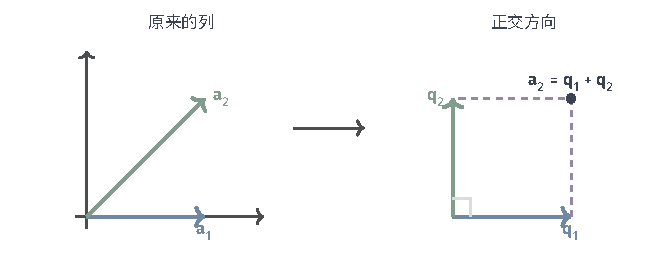
\includegraphics[width=112mm]{figures/00-shared/mathematical-preliminaries-upper/02-linear-spaces/tikz/comprehension-additions/linear-qr-columns.pdf}
  \caption{QR分解把列的方向和组合系数分开。取$\bm a_1=(1,0)^\top$、$\bm a_2=(1,1)^\top$，
  正交化得到$\bm q_1=(1,0)^\top$、$\bm q_2=(0,1)^\top$，并有$\bm a_1=\bm q_1$、
  $\bm a_2=\bm q_1+\bm q_2$，故$\bm R=\left[\begin{smallmatrix}1&1\\0&1\end{smallmatrix}\right]$。
  虚线补出第二列的分量。}
  \label{fig:vol1-add-linear-qr-columns}
\end{figure}

这一分解的用处在于，涉及列空间的计算可以改在标准正交的$\bm Q$上进行，坐标由内积直接读出，不必再解Gram方程。第~\ref{chap:linear-solution-selection}章与第~\ref{chap:direct-linear-solvers}章解方程与最小二乘问题时就是这样使用它的。

\subsubsection{列相关时的处理}

定理~\ref{thm:ls-gram-schmidt}要求各列线性无关。若不满足，某一步会出现$\bm u_j=\bm0$。由正交分解，这恰好说明$\bm a_j$已在前面方向张成的空间中，没有带来新方向。这时不能对零向量归一化，应跳过这一列，只在$\bm R$中记下它的系数$\langle\bm a_j,\bm q_i\rangle$。跳过它不影响后续各列，因为张成的空间没有变。

全部处理完以后，留下的$\bm q$的个数等于列空间的维数$r=\operatorname{rank}\bm A$，仍有$\bm A=\bm Q\bm R$。其中$\bm Q\in\mathbb R^{m\times r}$的列是列空间的标准正交基；$\bm R\in\mathbb R^{r\times d}$各行从左到右第一个非零元的位置逐行右移。$r<d$时$\bm R$不是方阵，不能求逆。下面是最小的例子。
\begin{example}[列相关时跳过零余量]
\label{ex:ls-qr-dependent-columns}
设$\bm A=[\bm a_1\ \bm a_2]$，其中$\bm a_1=(1,0)^\top$、$\bm a_2=(2,0)^\top$，第二列是第一列的两倍。$\bm a_1$已是单位向量，$\bm q_1=\bm a_1$。处理第二列时，$\langle\bm a_2,\bm q_1\rangle=2$，扣除后$\bm u_2=\bm a_2-2\bm q_1=\bm0$：第二列没有带来新方向。于是跳过$\bm a_2$，只在$\bm R$中记下系数$2$，得到$r=1$，
\[
\begin{gathered}
\bm Q=\begin{bmatrix}1\\0\end{bmatrix},\\
\bm R=\begin{bmatrix}1&2\end{bmatrix},\\
\bm Q\bm R=\begin{bmatrix}1&2\\0&0\end{bmatrix}=\bm A .
\end{gathered}
\]
乘回去仍得到$\bm A$，说明跳过的列并没有丢失信息，它的系数保存在$\bm R$中。列空间是$x$轴，$\bm Q$的唯一一列构成它的标准正交基，留下的列数$1$正是$\operatorname{rank}\bm A$；$\bm R$是$1\times2$矩阵，不能求逆。
\end{example}
于是在精确算术下，同一过程也给出列空间的一组标准正交基与矩阵的秩。有限精度下，扣除后的余量很少恰好为零；怎样判断它“算作零”，以及怎样改写扣除顺序以减少正交性的损失，属于数值计算问题，在第~\ref{sec:ls-numerical-sensitivity}节讨论。

\subsection{正交投影}
\label{sec:ls-orthogonal-projection}

标准正交基使子空间中的分量可以逐个读出。把这些分量合在一起，就得到正交投影。本小节证明它是子空间中离原向量最近的点，再把它写成矩阵，并给出判断一个矩阵是否为正交投影的方法。

\paragraph{向子空间的正交分解}
若$\bm q_1,\ldots,\bm q_r$是子空间$U$的标准正交基，引理~\ref{lem:ls-orthogonal-decomposition}中的Gram矩阵是单位矩阵，Gram方程直接给出$\bm a=(\langle\bm q_i,\bm x\rangle)_i$。于是分解可以直接写出：
\begin{equation}
 \bm x=\underbrace{\sum_{j=1}^r\langle\bm x,\bm q_j\rangle\bm q_j}_{\bm u\in U}+\underbrace{\Bigl(\bm x-\sum_{j=1}^r\langle\bm x,\bm q_j\rangle\bm q_j\Bigr)}_{\bm r\in U^\perp}.
 \label{eq:ls-orthonormal-projection}
\end{equation}
$\bm u$称为$\bm x$在$U$上的正交投影。$\bm u$与$\bm r$正交，由勾股定理，
\[
 \lVert\bm x\rVert^2=\lVert\bm u\rVert^2+\lVert\bm r\rVert^2\geq\sum_{j=1}^r\langle\bm x,\bm q_j\rangle^2.
\]
即沿一部分标准正交方向读出的系数，其平方和不超过总长度的平方；等号恰在$\bm x\in U$时成立。

现在证明$\bm u$是最近点。对任意$\bm v\in U$，$\bm x-\bm v=(\bm x-\bm u)+(\bm u-\bm v)$的两项分别属于$U^\perp$和$U$。由勾股定理，
\[
 \lVert\bm x-\bm v\rVert^2=\lVert\bm x-\bm u\rVert^2+\lVert\bm u-\bm v\rVert^2\geq\lVert\bm x-\bm u\rVert^2.
\]
等号只在$\bm v=\bm u$时成立，所以$\bm u$是唯一的最近点。基不是标准正交时，同样可以先解Gram方程求出投影；实际求解时不必显式形成逆矩阵。

最近点的唯一性来自内积确定的正交分解。第~\ref{sec:ls-quotient-norms}节已经证明一般范数下最近点存在，示例~\ref{ex:ls-linf-nonunique-nearest}却在$\ell_\infty$范数下给出了无穷多个最近点；同一个点在欧氏范数下的最近点只有原点，因为$\lVert\bm y-(t,0)^\top\rVert_2^2=t^2+1$只在$t=0$时取最小值。

下面用标准正交基重算前面的正交分解。
\begin{example}[用标准正交基重算正交分解]
\label{ex:ls-orthonormal-projection-line}
回到示例~\ref{ex:ls-orthogonal-decomposition-line}的$\bm y=(1,1.1,0.9)^\top$与直线$U$，这次先把方向向量归一化为$\bm q_1=(1,1,1)^\top/\sqrt3$，于是$U=\operatorname{span}\{\bm q_1\}$。投影系数就是一次内积$\langle\bm y,\bm q_1\rangle=3/\sqrt3=\sqrt3$，投影为$\sqrt3\,\bm q_1=(1,1,1)^\top$，余量为$(0,0.1,-0.1)^\top$，它与$\bm q_1$正交。结果与前例相同，但这里不需要解Gram方程：归一化已经把Gram矩阵变成了$1$。由上面的最近点性质，$(1,1,1)^\top$还是直线$U$上离$\bm y$最近的点。
\end{example}

\paragraph{投影矩阵}
\label{sec:ls-projection-matrices}
正交投影随原向量线性变化。记$\bm y$在$U$上的正交投影为$\bm p$。$\bm y_1,\bm y_2$的正交分解相加、数乘后仍是正交分解，由分解的唯一性，投影也随之相加、数乘。所以$\bm y\mapsto\bm p$是一个线性映射，称为到$U$的正交投影。

在欧氏内积下，它可以写成矩阵。设$\bm Q$的列是$U$的标准正交基。由$\bm p=\sum_j\langle\bm q_j,\bm y\rangle\bm q_j=\bm Q\bm Q^\top\bm y$，到$U$的正交投影是
\begin{equation}
\begin{gathered}
\bm P_U=\bm Q\bm Q^\top,\\
\bm P_U^\top=\bm P_U,\\
\bm P_U^2=\bm P_U.
\end{gathered}
\label{eq:linear-algebra-orthogonal-projector}
\end{equation}
两条性质都可以直接验证。由$\bm Q^\top\bm Q=\bm I$，$\bm P_U^2=\bm Q(\bm Q^\top\bm Q)\bm Q^\top=\bm Q\bm Q^\top$，即幂等：已经在$U$中的点再投影一次不变。$(\bm Q\bm Q^\top)^\top=\bm Q\bm Q^\top$，即对称：内积中可以把投影移到另一侧。此外$\operatorname{range}\bm P_U=\operatorname{range}\bm Q=U$。$\bm Q$不是方阵时，$\bm P_U$通常不是单位矩阵，它只保留$U$中的分量。

\paragraph{正交投影、斜投影与幂等}
拿到一个矩阵，怎样判断它是不是正交投影？幂等性只说明它是某种投影，不说明它给出最近点。一般的幂等矩阵$\bm P$把$\bm y$分成$\bm P\bm y$与$\bm y-\bm P\bm y$两部分，前者在像中，后者在零空间中，因为$\bm P(\bm y-\bm P\bm y)=\bm P\bm y-\bm P^2\bm y=\bm0$。但两部分不必正交。这种映射称为\term{斜投影}（oblique projection）。

\begin{example}[反例：幂等而不对称的投影]
\label{ex:ls-oblique-projection}
取
\[
 \bm P=\begin{bmatrix}1&-1\\0&0\end{bmatrix}.
\]
直接相乘得$\bm P^2=\bm P$，所以它幂等；它把$(y_1,y_2)^\top$送到$x$轴上的$(y_1-y_2,0)^\top$。残差$\bm y-\bm P\bm y=(y_2,y_2)^\top$与$x$轴方向$(1,0)^\top$的内积是$y_2$，$y_2\neq0$时不为零，所以$\bm P\bm y$不是$x$轴上离$\bm y$最近的点。这个$\bm P$也不对称：$\bm P^\top\neq\bm P$。
\end{example}

对称性正是正交的条件。若$\bm P$幂等且对称，对任意$\bm y,\bm z$有
\[
 (\bm y-\bm P\bm y)^\top\bm P\bm z=\bm y^\top(\bm P-\bm P^\top\bm P)\bm z=\bm y^\top(\bm P-\bm P^2)\bm z=0,
\]
即残差与整个像正交。于是$\bm y=\bm P\bm y+(\bm y-\bm P\bm y)$是$\bm y$关于像空间的正交分解，由分解的唯一性，$\bm P$就是到其像的正交投影。所以判别分两步：先验幂等，判断是不是投影；再验对称，判断是不是正交投影。

\section{线性泛函的内积表示与伴随}
\label{sec:ls-adjoints}

第~\ref{sec:ls-dual-spaces}节的读取规则属于对偶空间，与被读取的向量不在同一个空间；转置在那里是对偶映射的矩阵。有了内积，每个读取都可以写成与一个固定向量的内积，对偶映射也就变成内积空间之间的映射，称为伴随。第~\ref{sec:ls-orthogonality}节证明四个基本子空间的正交关系时，用到的正是伴随在欧氏内积下的形式：内积左侧的$\bm A$可以改写成右侧的$\bm A^\top$。

\subsection{线性泛函的内积表示}
\phantomsection
\label{sec:ls-riesz-representation}
在$\mathbb R^d$的欧氏内积下，加权读取$\varphi(\bm x)=\bm a^\top\bm x$就是与向量$\bm a$的内积。在一般有限维内积空间中，每个读取也都能这样写。
\begin{theorem}[有限维Riesz表示定理]
\label{thm:ls-riesz-representation}
设$V$是有限维内积空间。对每个$\varphi\in V^*$，存在唯一的$\bm v_\varphi\in V$，使$\varphi(\bm x)=\langle\bm x,\bm v_\varphi\rangle$对所有$\bm x\in V$成立。
\end{theorem}
\begin{proof}
取$V$的一组标准正交基$\bm q_1,\ldots,\bm q_d$（第~\ref{sec:ls-orthonormal-basis-construction}节），令$\bm v_\varphi=\sum_j\varphi(\bm q_j)\bm q_j$。由式~\eqref{eq:ls-orthonormal-expansion}，$\bm x=\sum_j\langle\bm x,\bm q_j\rangle\bm q_j$，于是
\[
 \varphi(\bm x)=\sum_j\langle\bm x,\bm q_j\rangle\varphi(\bm q_j)=\Bigl\langle\bm x,\sum_j\varphi(\bm q_j)\bm q_j\Bigr\rangle=\langle\bm x,\bm v_\varphi\rangle.
\]
若$\bm v,\bm v'$都满足要求，则$\langle\bm x,\bm v-\bm v'\rangle=0$对一切$\bm x$成立，取$\bm x=\bm v-\bm v'$得$\bm v=\bm v'$。
\end{proof}
对应$\varphi\mapsto\bm v_\varphi$保持线性组合，这由表示向量的唯一性得到；每个$\bm v$又都表示读取$\langle\cdot,\bm v\rangle$。所以这个对应是$V^*$到$V$的双射。在它之下，标准正交基的对偶基就是这组基本身，因为第$j$个坐标读取是$\bm x\mapsto\langle\bm x,\bm q_j\rangle$。对一般的基，对偶基对应的向量与原基不同：图~\ref{fig:ls-dual-basis-readout}中的红色箭头$\bm b^1,\bm b^2$，正是对偶读取$\varphi_1,\varphi_2$在欧氏内积下对应的向量。

表示向量依赖内积，读取本身却不依赖。在$\mathbb R^d$上取加权内积$\langle\bm x,\bm y\rangle_{\bm M}=\bm x^\top\bm M\bm y$，同一个读取$\varphi(\bm x)=\bm a^\top\bm x=\bm x^\top\bm M(\bm M^{-1}\bm a)$对应的向量是$\bm M^{-1}\bm a$，而不是$\bm a$。函数空间中也是如此。
\begin{example}[积分读取在两点内积下的表示向量]
\label{ex:ls-riesz-integral-two-point}
在$P_1$上取两点内积$\langle f,g\rangle=f(0)g(0)+f(1)g(1)$，考虑积分读取$\varphi(f)=\int_0^1f(t)\,\mathrm dt$。对$f=a+bt$，$\varphi(f)=a+b/2$。要把它写成与某个固定函数的内积，而这个内积只用到$f(0)=a$与$f(1)=a+b$，所以先把$a+b/2$表示成这两个值的组合：$a+b/2=\tfrac12\bigl(f(0)+f(1)\bigr)$。这正是$f$与常数函数$\tfrac12$的内积：
\[
 \Bigl\langle f,\tfrac12\Bigr\rangle=\tfrac12\bigl(f(0)+f(1)\bigr)=\tfrac12(a+a+b)=a+\frac b2 .
\]

因此$\bm v_\varphi$是常数函数$\tfrac12$。在系数向量的欧氏内积下，同一个读取对应$(1,1/2)^\top$，表示向量随内积而变。等式$\varphi(f)=\tfrac12\bigl(f(0)+f(1)\bigr)$也说明梯形公式对一次函数精确。
\end{example}
表示向量还给出读取的大小。由Cauchy--Schwarz不等式，$|\varphi(\bm x)|\leq\lVert\bm x\rVert\,\lVert\bm v_\varphi\rVert$；$\bm v_\varphi\neq\bm0$时，取$\bm x=\bm v_\varphi/\lVert\bm v_\varphi\rVert$可取到等号。所以仿照第~\ref{sec:ls-dual-norms}节，在单位球上取读取的最大值，得到
\[
 \lVert\varphi\rVert_*=\max_{\lVert\bm x\rVert\leq1}|\varphi(\bm x)|=\lVert\bm v_\varphi\rVert .
\]
在$\mathbb R^d$的欧氏内积下，这就是$\ell_2$范数的对偶范数仍为$\ell_2$范数。

\subsection{伴随与特殊线性算子}
对偶映射把输出端的读取$f$传回输入端，得到读取$f\circ T$。若把两端的读取都换成表示它的向量，就得到伴随。
\begin{definition}[伴随]
\label{def:linear-algebra-adjoint}
设$T:V\to W$是两个有限维实内积空间之间的线性映射。若存在$T^\star:W\to V$使
\begin{equation}
 \langle T\bm x,\bm y\rangle_W=\langle\bm x,T^\star\bm y\rangle_V
 \label{eq:ls-adjoint-pairing}
\end{equation}
对所有$\bm x\in V$、$\bm y\in W$成立，则$T^\star$称为$T$的\term{伴随}（adjoint）。
\end{definition}

伴随总存在且唯一。固定$\bm y\in W$，$\bm x\mapsto\langle T\bm x,\bm y\rangle_W$是$V$上的线性泛函。由定理~\ref{thm:ls-riesz-representation}，存在唯一的向量使它写成与该向量的内积，把这个向量记为$T^\star\bm y$。$T^\star$对$\bm y$线性：
\[
 \langle\bm x,aT^\star\bm y+bT^\star\bm y'\rangle_V=a\langle T\bm x,\bm y\rangle_W+b\langle T\bm x,\bm y'\rangle_W=\langle T\bm x,a\bm y+b\bm y'\rangle_W,
\]
由表示向量的唯一性，$T^\star(a\bm y+b\bm y')=aT^\star\bm y+bT^\star\bm y'$。

用对偶映射的语言说，把$\bm y\in W$看成读取$\langle\cdot,\bm y\rangle_W$，则$T'$把它送到读取$\langle T\,\cdot,\bm y\rangle_W=\langle\cdot,T^\star\bm y\rangle_V$。所以伴随就是借内积把读取换成向量以后的对偶映射。

具体计算时，取$V,W$的基。由坐标下的内积公式，两边的内积写成$\langle\bm x,\bm x'\rangle_V=\bm x^\top\bm M_V\bm x'$、$\langle\bm y,\bm y'\rangle_W=\bm y^\top\bm M_W\bm y'$，这里$\bm x,\bm y$等指坐标，$\bm M_V,\bm M_W$是两组基的Gram矩阵，对称正定因而可逆。设$T$的矩阵为$\bm A$，伴随的矩阵为$\bm B$。式~\eqref{eq:ls-adjoint-pairing}要求$(\bm A\bm x)^\top\bm M_W\bm y=\bm x^\top\bm M_V\bm B\bm y$对所有$\bm x,\bm y$成立。取$\bm x,\bm y$为标准坐标向量逐个比较元素，这等价于$\bm A^\top\bm M_W=\bm M_V\bm B$，即
\begin{equation}
 \bm B=\bm M_V^{-1}\bm A^\top\bm M_W.
 \label{eq:ls-weighted-adjoint}
\end{equation}
两端都取标准正交基时，$\bm M_V,\bm M_W$都是单位矩阵，伴随矩阵就是$\bm A^\top$，与对偶映射的矩阵相同。一般情形下，伴随既不是单纯转置，也不是转置再求逆。下面的例子说明这一点。
\begin{example}[加权内积下的伴随]
\label{ex:ls-weighted-adjoint}
设$V=W=\mathbb R^2$都取加权内积$\langle\bm x,\bm y\rangle_{\bm M}=\bm x^\top\bm M\bm y$，$\bm M=\operatorname{diag}(4,1)$，并考虑把第二个坐标移到第一个位置的映射$T\bm x=\bm A\bm x$，其中
\[
 \bm A=\begin{bmatrix}0&1\\0&0\end{bmatrix}.
\]
标准基在这个内积下不是标准正交基，所以伴随要用式~\eqref{eq:ls-weighted-adjoint}计算：
\[
 \bm B=\bm M^{-1}\bm A^\top\bm M
 =\begin{bmatrix}1/4&0\\0&1\end{bmatrix}\begin{bmatrix}0&0\\1&0\end{bmatrix}\begin{bmatrix}4&0\\0&1\end{bmatrix}
 =\begin{bmatrix}0&0\\4&0\end{bmatrix}.
\]
再回到配对等式核对：$\bm A\bm x=(x_2,0)^\top$，$\langle\bm A\bm x,\bm y\rangle_{\bm M}=4x_2y_1$；$\bm B\bm y=(0,4y_1)^\top$，$\langle\bm x,\bm B\bm y\rangle_{\bm M}=x_2\cdot4y_1$，两者相等。因数$4$来自输出落在权重为$4$的第一个坐标上，伴随要把这个权重带回输入端。所以伴随矩阵是$\bm B$，而不是$\bm A^\top$：
\[
 \bm B=\begin{bmatrix}0&0\\4&0\end{bmatrix}\neq\begin{bmatrix}0&0\\1&0\end{bmatrix}=\bm A^\top.
\]
\end{example}
对偶映射的矩阵总是$\bm A^\top$；伴随与它的差别，来自读取与向量之间的对应$\bm a\mapsto\bm M^{-1}\bm a$随内积改变。四个基本子空间正交关系的证明只用到配对恒等式，所以在一般内积空间中同样有$\ker T^\star=(\operatorname{im}T)^\perp$、$\ker T=(\operatorname{im}T^\star)^\perp$。

\paragraph{伴随的运算规则}
由配对定义可以逐条推出伴随的运算规则：
\[
 \begin{gathered}
(T+S)^\star=T^\star+S^\star,\\
(cT)^\star=c\,T^\star,\\
(TS)^\star=S^\star T^\star,\\
T^{\star\star}=T.
 \end{gathered}
\]
例如$\langle TS\bm x,\bm y\rangle=\langle S\bm x,T^\star\bm y\rangle=\langle\bm x,S^\star T^\star\bm y\rangle$，复合的伴随与乘积的转置一样反转次序；恒等映射的伴随是自身。图~\ref{fig:ls-adjoint-action-transfer}画出伴随怎样把配对从输出端搬回输入端。

伴随不是逆：逆把输出复原成输入，伴随只把作用从内积的一侧移到另一侧。
\begin{example}[反例：伴随不是逆]
\label{ex:ls-adjoint-not-inverse}
最简单的反例是非零内积空间$V$上的放大两倍$T=2\operatorname{id}$。数乘可以从内积的一侧移到另一侧，$\langle2\bm x,\bm y\rangle=\langle\bm x,2\bm y\rangle$对一切$\bm x,\bm y$成立，所以$T^\star=2\operatorname{id}$：伴随仍是放大两倍。复原输入的逆却是缩小一半，$T^{-1}=\tfrac12\operatorname{id}$。因此$T^\star\neq T^{-1}$。两者相等恰好是正交算子的条件，下面马上会遇到。
\end{example}
\begin{figure}[!htb]
  \centering
  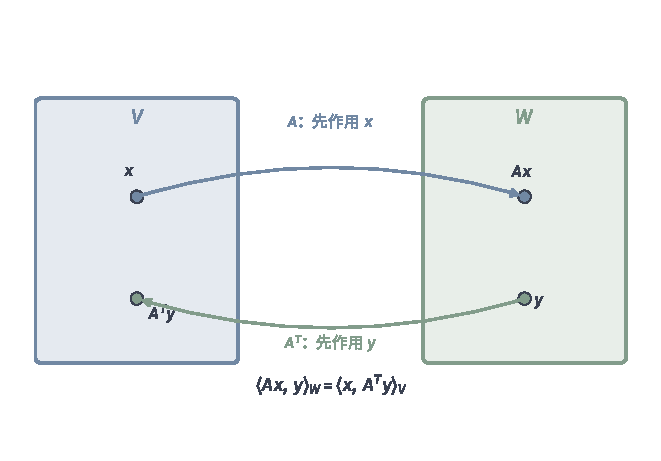
\includegraphics[width=112mm]{figures/00-shared/mathematical-preliminaries-upper/02-linear-spaces/matplotlib/ls-adjoint-action-transfer/ls-adjoint-action-transfer.pdf}
  \caption{内积伴随把输出端的配对搬回输入端。左：$T:V\to W$把$\bm x$映成$T\bm x$，与$\bm y\in W$配对；右：伴随$T^\star:W\to V$把$\bm y$映回$T^\star\bm y\in V$，使$\langle T\bm x,\bm y\rangle_W=\langle\bm x,T^\star\bm y\rangle_V$。标准欧氏内积下$T^\star$就是转置；它反转的是配对的方向，不是逆作用。箭头与空间为解析示意。}
  \label{fig:ls-adjoint-action-transfer}
\end{figure}

\paragraph{自伴、正交与正规算子}
对算子$T:V\to V$，伴随仍是$V$上的算子，可以与$T$比较。下面四类算子都由$T$与$T^\star$之间的一个等式规定。

若$T^\star=T$，称$T$为\term{自伴}（self-adjoint）算子，它在标准正交基下对应对称矩阵。若$T^\star=-T$，称$T$为\term{反自伴}（skew-adjoint）算子，它在标准正交基下对应满足$\bm A^\top=-\bm A$的反对称矩阵。反自伴算子把每个向量送到与它正交的方向：由$\langle T\bm x,\bm x\rangle=\langle\bm x,T^\star\bm x\rangle=-\langle\bm x,T\bm x\rangle$得$\langle T\bm x,\bm x\rangle=0$。例如平面上的$\left[\begin{smallmatrix}0&-1\\1&0\end{smallmatrix}\right]$把$(x_1,x_2)^\top$送到$(-x_2,x_1)^\top$，即逆时针旋转直角。

若$Q^\star Q=\operatorname{id}$，则$Q$保持内积：$\langle Q\bm x,Q\bm y\rangle=\langle\bm x,Q^\star Q\bm y\rangle=\langle\bm x,\bm y\rangle$，称为正交算子。它在标准正交基下对应第~\ref{sec:ls-orthogonal-matrices}节的正交矩阵；由方阵的单侧逆即双侧逆，$Q^{-1}=Q^\star$。

满足$TT^\star=T^\star T$的算子称为\term{正规}（normal）算子，即$T$与自己的伴随可交换。自伴、反自伴与正交算子都是正规算子：前两种情形$T^\star=\pm T$显然与$T$交换，正交算子满足$QQ^\star=Q^\star Q=\operatorname{id}$。一般算子未必正规，例如示例~\ref{ex:ls-weighted-adjoint}中的$\bm A=\left[\begin{smallmatrix}0&1\\0&0\end{smallmatrix}\right]$在欧氏内积下满足$\bm A\bm A^\top=\operatorname{diag}(1,0)\neq\operatorname{diag}(0,1)=\bm A^\top\bm A$。这些算子的谱性质在第~\ref{chap:eigen-spectral-decomposition}章讨论，这里只给出定义。

\paragraph{复空间中的泛函表示与伴随}
复空间沿用前面“第一变量共轭线性、第二变量线性”的约定。这时线性泛函应写成$\varphi(\bm x)=\langle\bm v,\bm x\rangle$，让$\bm x$处于线性的变量位置。若$\bm q_1,\ldots,\bm q_d$是标准正交基，则$\bm v=\sum_j\overline{\varphi(\bm q_j)}\bm q_j$；代入各基向量即可核对读数。表示向量随泛函作共轭线性变化，这与实空间中的线性对应不同。

例如在$\mathbb C$的标准内积$\langle v,z\rangle=\overline v z$下，泛函$\varphi(z)=(1+\mathrm i)z$对应$v=1-\mathrm i$，因为$\overline v z=(1+\mathrm i)z$。若交换两个变量的位置，得到的表达式关于$z$共轭线性，不再是线性泛函。所以共轭来自内积约定，不能从实数公式中直接删去。

两个复内积空间之间的伴随仍由$\langle T\bm x,\bm y\rangle_W=\langle\bm x,T^\star\bm y\rangle_V$定义。在标准正交基下，若$T$的矩阵为$\bm A$，伴随的矩阵就是$\bm A^*$；若两端基的Gram矩阵为$\bm M_V,\bm M_W$，则为$\bm M_V^{-1}\bm A^*\bm M_W$。这与代数对偶映射的矩阵$\bm A^\top$不同：后者只复合线性泛函，不涉及内积和共轭。复空间中，自伴矩阵满足$\bm A=\bm A^*$；保持内积的方阵满足$\bm A^*\bm A=\bm I$，称为酉矩阵。

\section{本章小结}
\label{sec:ls-normed-inner-product-summary}

本章回答了章首的三个问题：两个向量相差多少，一列近似是否趋于极限，两个方向是否垂直。前两个问题由范数回答，第三个问题需要内积。

范数给向量规定大小，从而可以度量误差。常用坐标范数之间满足$\lVert\bm x\rVert_q\leq\lVert\bm x\rVert_p\leq d^{1/p-1/q}\lVert\bm x\rVert_q$（$p\leq q$），比较常数依赖维数，所以同一个误差在不同范数下的读数不同。

有了范数就能谈收敛与连续。向量列与矩阵列的收敛等价于逐坐标、逐元素收敛；映射的联合极限要求所有趋近方式给出同一结果，只检查若干路径只能否定、不能证明极限存在。闭有界集上的连续函数取到最值并且一致连续，闭性、有界性与连续性三个条件缺一不可。

有限维结构带来更强的结论。任意两个范数等价，所以收敛、连续与柯西性质都不依赖所选范数，变的只是误差的数值和比较常数。有限维赋范空间完备，是Banach空间，子空间都是闭集；绝对收敛的向量与矩阵级数收敛，并有尾和估计。诱导矩阵范数给出线性映射的最大放大倍数，有限维线性映射因而都Lipschitz连续；对偶范数把输入误差的限制转化为线性读取的最大变化；商范数衡量忽略一个子空间中的差别以后剩余的大小。一般范数下向子空间的最近点存在，但可能不唯一。

内积进一步给出长度、夹角和正交。内积诱导的长度是范数，但并非每个范数都来自内积，平行四边形恒等式可以检验这一点；有限维内积空间是Hilbert空间。Gram矩阵记录一组向量的两两内积，它总是半正定的，并且恰在这组向量线性无关时正定；反过来，每个半正定矩阵都是某组向量的Gram矩阵，这又推出逐元素乘积保持半正定。

正交分解把向量拆成子空间中的部分与垂直的部分，正交投影是内积诱导距离下唯一的最近点；矩阵是正交投影，当且仅当它幂等且对称。标准正交基使坐标可以由内积直接读出，并保持长度；Gram--Schmidt正交化保证这样的基总存在，QR分解把这一过程写成矩阵形式。线性泛函的内积表示与伴随，把上一章的代数对偶与本章的几何结构联系起来：在标准正交基下伴随就是转置，在一般基下还要计入两端的Gram矩阵。

这些结论都依赖有限维：范数等价、完备性与最近点存在的证明，都用到了有限个坐标或闭有界集上的最值。它们为后续各章提供共同依据。第~\ref{chap:eigen-spectral-decomposition}章在正交换基下寻找线性作用的简单表示，正交矩阵与自伴算子在那里尤为重要；矩阵幂和级数使用收敛与次乘性，迭代使用完备性和误差估计，多元微分把局部变化表示为线性映射并用算子范数控制余项。

